\section{模型的建立与求解}
本文按照原始素材处理与特征预测两个阶段组织数据。附件1的100条视频用于自主提取三模态特征，视频、音轨与官方转写通过样本标识关联；附件2的对齐版特征用于情感预测模型训练和评价，附件3的同版本特征用于专项推理。各阶段保留全部样本，通过内容掩码、观测掩码与截断记录描述有效范围。问题二的标准化参数仅由附件2训练集的观测位置估计。

\subsection{问题一的模型建立与求解}
\label{sec:q1}
\subsubsection{问题分析与建模思路}

附件1提供100条英文视频及对应转写文本。问题一要求从原始素材中提取文本、语音和视觉特征，并建立三类特征与原始片段之间可核验的时间对应关系。本问旨在构造具有统一时序组织、明确有效范围和完整溯源记录的多模态表示，为后续分析提供可解释的数据基础。

三种模态的时间结构存在差异：文本以离散词元组织，语音是连续采样信号，视觉则由带时间戳的视频帧组成。直接按序号拼接会混淆不同时间范围内的信息；按词数均分视频长度又会忽略语速、停顿和词长差异。此外，人脸未检出和文本接口截断均可能使部分位置缺少特征，必须与正常观测区分。

据此，本文采用\textbf{以原词为时间锚点、以子词为输出位置}的建模方案：首先利用官方转写与音频建立词级时间区间，再将子词映射到父词；在同一锚点区间内，对语音和视觉帧特征进行时间交叠加权聚合。进一步计算覆盖率与边界扰动敏感度，形成不确定边界锚点对齐模型（Uncertain-Boundary Anchor Alignment，UBA）。图\ref{q1:fig:flow}给出总体流程。

\begin{figure}[htbp]
\centering
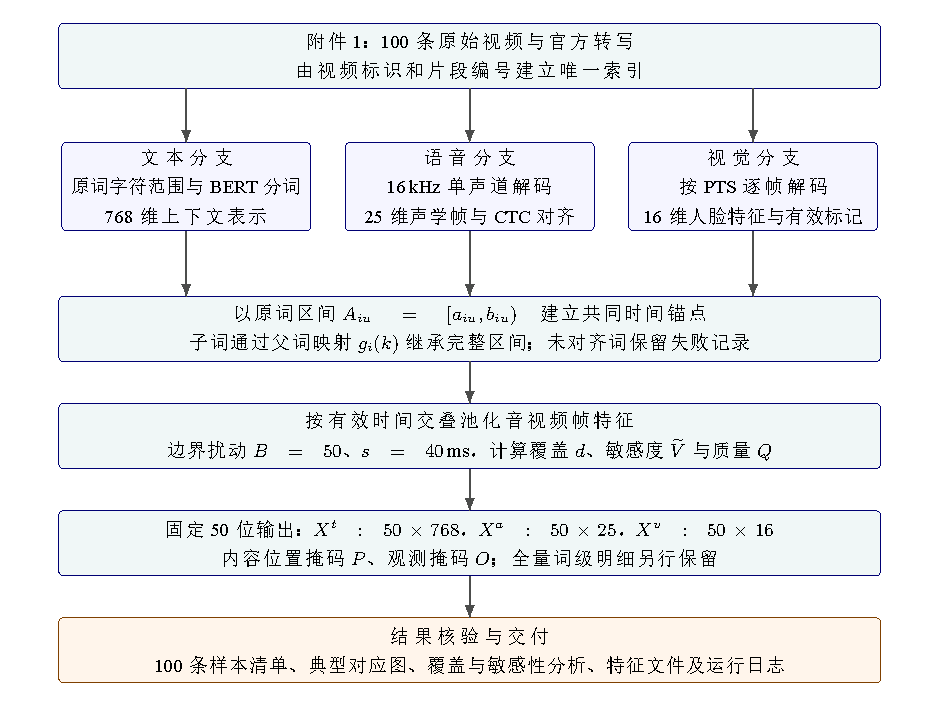
\includegraphics[width=\linewidth]{figures/q1_flowchart.pdf}
\caption{三模态特征提取与时间锚点对齐流程。声学特征与强制对齐共用音频信号；视觉帧采用自身解码时间戳。}
\label{q1:fig:flow}
\end{figure}

输出采用50位定长接口，每个内容位置通过父词索引关联实际时间区间。模型评价包括样本覆盖、区间结构、模态观测覆盖与参数敏感性四个方面。

\subsubsection{数据准备}
\label{q1:sec:data}

\paragraph{样本组织与数据特征}

以视频标识与片段编号组成唯一键\file{video\_id\$\_\$clip\_id}，连接视频文件、官方转写和输出记录。附件1共来自37个原始视频，包含1932个空白分隔原词和2317个BERT词元；完整文本中283个原词对应多个词元，占14.65\%。样本标签仅用于数据说明，不参与本问的特征提取或参数拟合。

\begin{table}[htbp]
\centering\small
\caption{数据特点与相应处理方式}
\label{q1:tab:data}
\begin{tabularx}{\linewidth}{p{3.1cm}p{4.0cm}Y}
\toprule
对象 & 实测特点 & 处理方式 \\
\midrule
文本长度 & 每条5--65词，5--82个词元 & 保存全量词表，固定接口仅保留前48个内容词元 \\
音频格式 & 源采样率44.1\,kHz，单/双声道AAC & 统一解码为16\,kHz单声道信号 \\
视频采样 & 8种分辨率，帧间隔并非处处相同 & 使用逐帧PTS，不由帧数和标称帧率反推时间 \\
容器时间 & 90条声明帧数与实解帧数不同 & 区分媒体样本数、有效呈现时长与解码跨度 \\
视觉可观测性 & 4条全片未检出人脸，另有局部未检出 & 保存有效帧掩码，缺失帧不参与池化 \\
\bottomrule
\end{tabularx}
\end{table}

\paragraph{时间基准与有效区间}

音频解码、重采样和声道合并后得到信号 $x_i[n]$，采样率为 $f_s=16000$\,Hz，其相对时间为 $n/f_s$。声学描述符提取与词级强制对齐使用同一信号，避免两种音频处理链引入不同的时间原点。

视频第 $j$ 帧的呈现时间取解码PTS与时间基的乘积，记为 $t_{ij}$。100条样本首帧PTS均为0，23241个解码帧的PTS完整且单调。根据容器编辑列表确定有效呈现范围，以音频相对秒数和视频PTS建立名义公共时间轴，保持两轨各自的原始时间尺度。

容器媒体时长、编辑列表时长和解码跨度分别描述存储范围、有效呈现范围与实际样本范围。100条样本的有效视频、音频时长分别合计为\VideoDuration\,s和\AudioDuration\,s。声明视频帧数为33147，实解23241，二者差额主要由编辑列表限定的呈现范围解释。逐样本汇总采用有效呈现时长；实际音频处理总时长为777.0091\,s。

记两轨解码跨度之差为 $\Delta_i=T_i^a-T_i^v$。其均值为$-92.3$\,ms，绝对值中位数为91.3\,ms。该量仅表示时长差，不作为同步偏移的估计。

图\ref{q1:fig:dataset}给出样本长度与媒体时间分布。原词数具有长尾，因此在定长接口之外保留全量词级记录；音视频跨度及帧数统计存在差异，因此视觉分支采用实际解码帧与PTS建立时间支撑。
\begin{figure}[htbp]
\centering
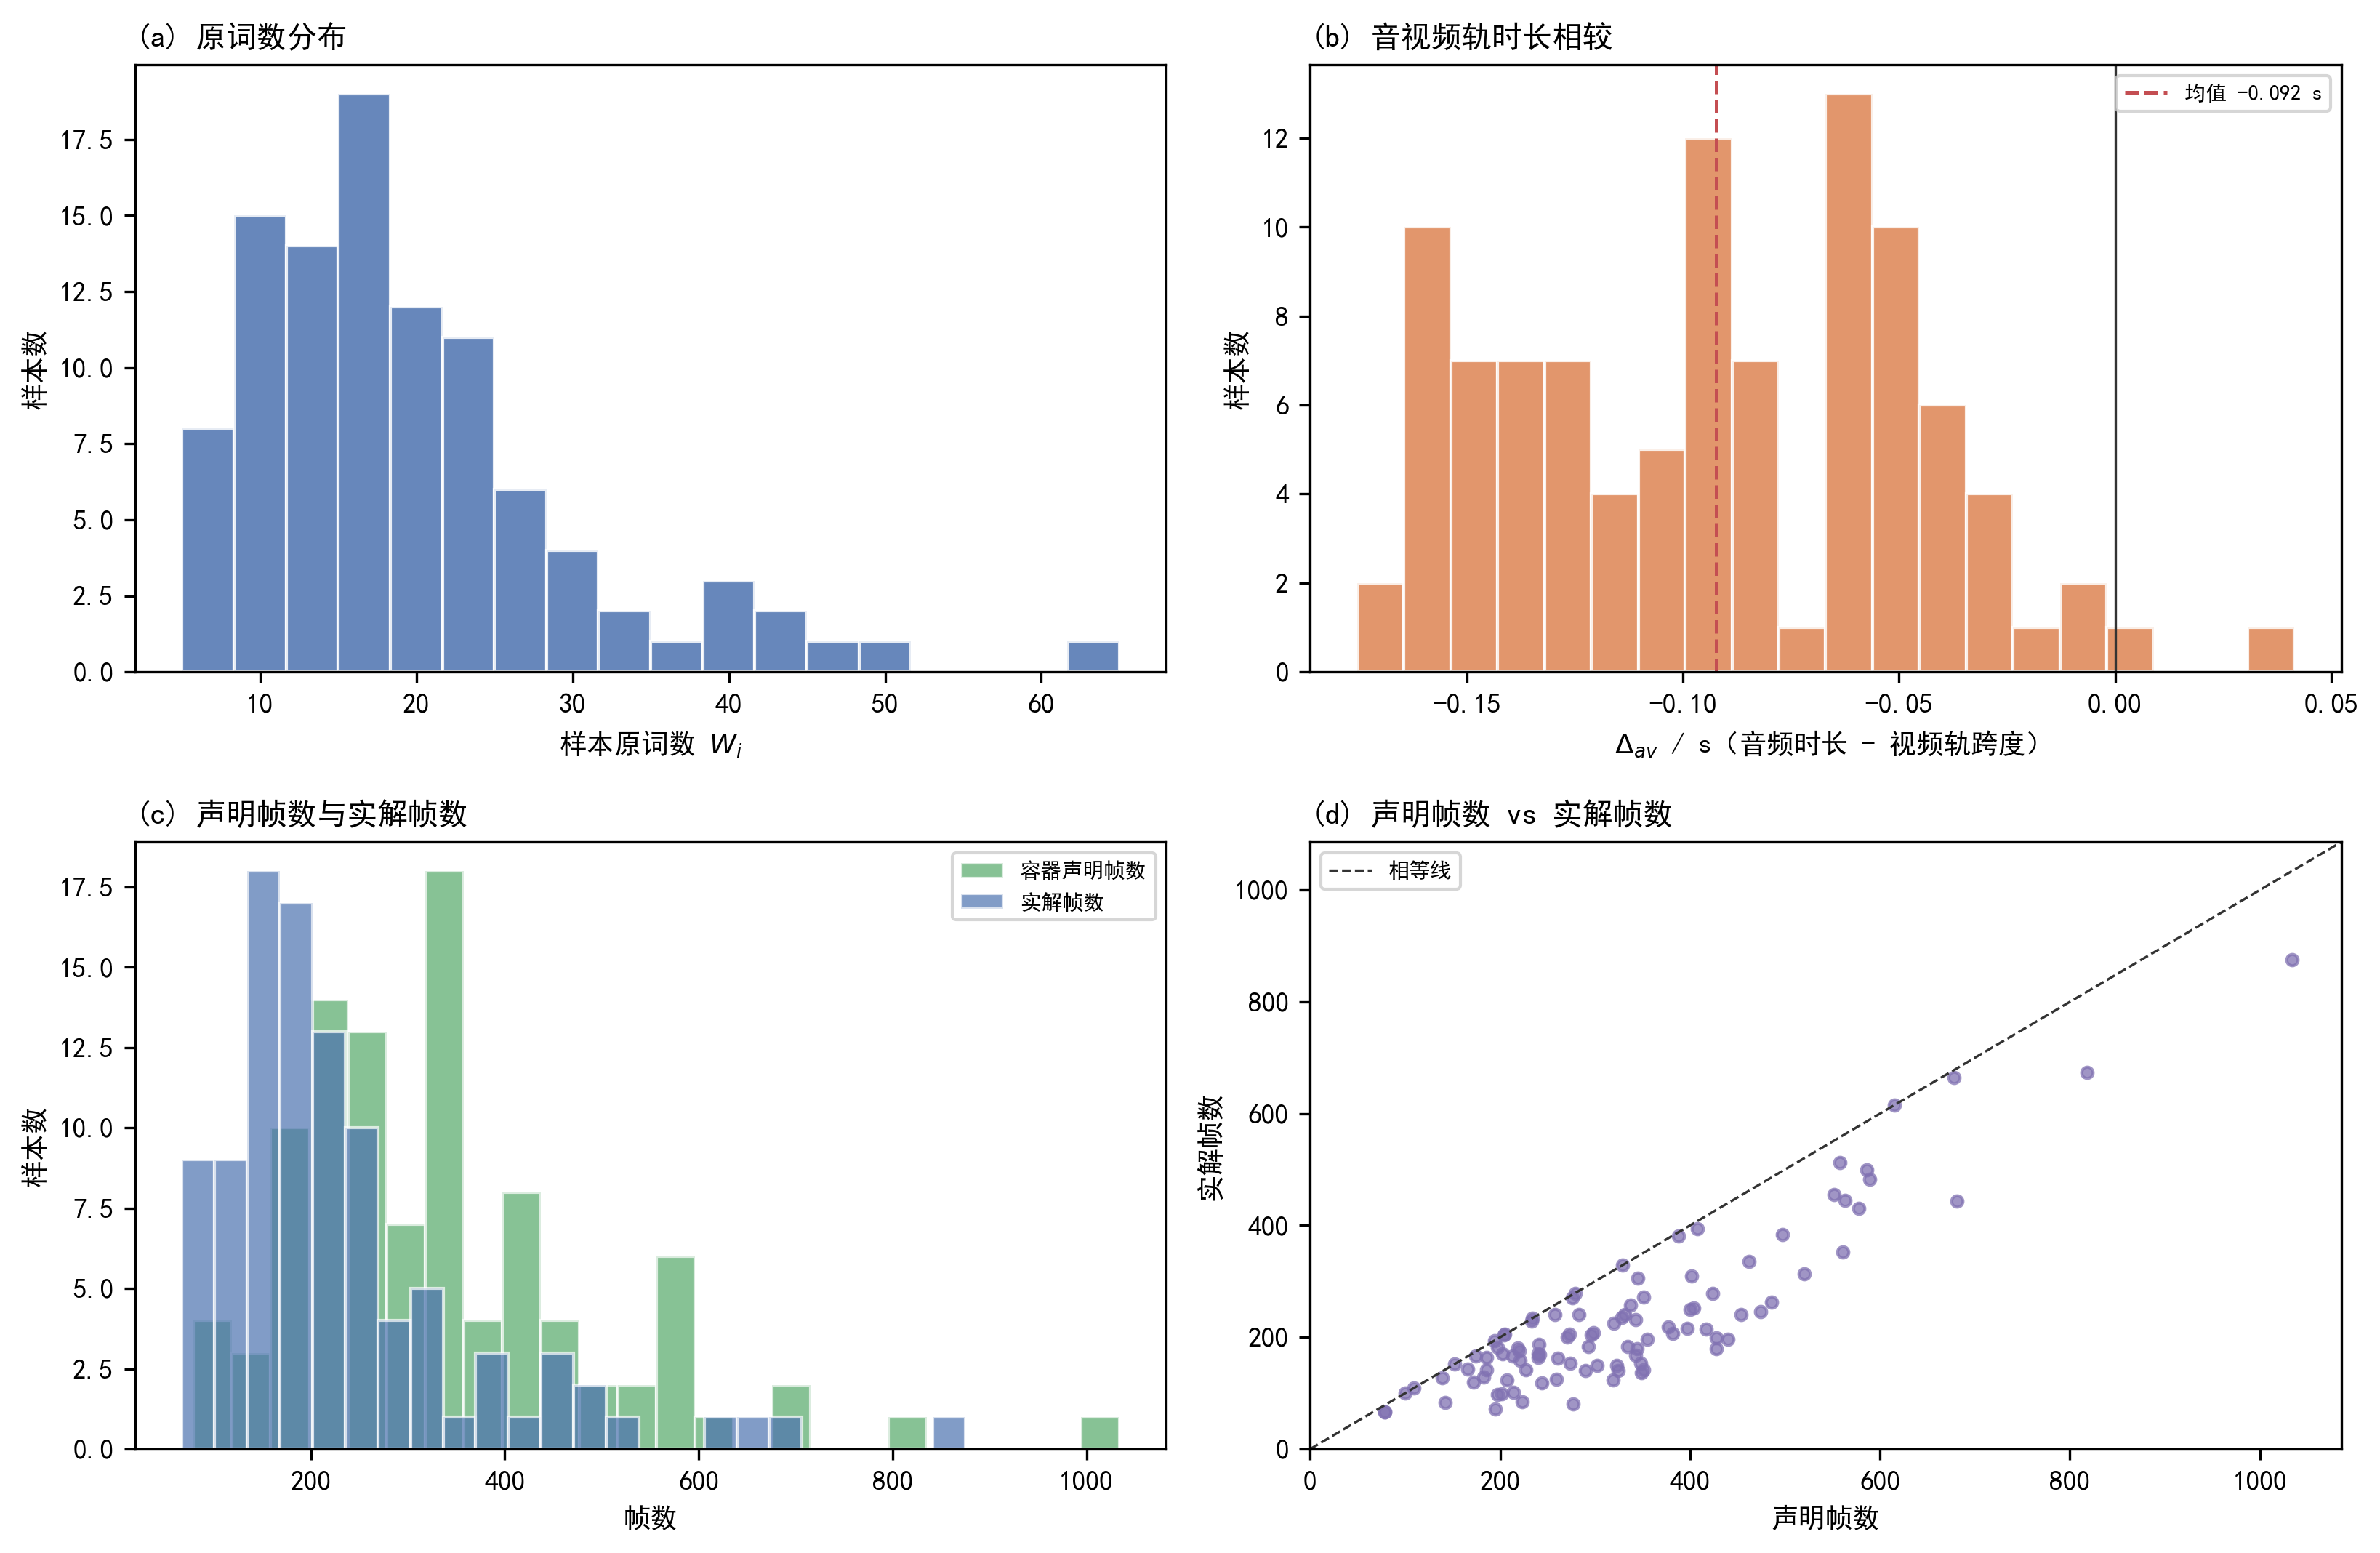
\includegraphics[width=\linewidth]{figures/q1_dataset.png}
\caption{附件1的原词数、音视频解码跨度差及帧数统计。声明帧数与实解帧数的差额主要与容器编辑列表有关。}
\label{q1:fig:dataset}
\end{figure}

\paragraph{建模约定}

以官方转写确定待对齐词序列，同一原词的子词共享其时间区间；视觉描述符取自成功检测的人脸，质量分数用于评价锚点的相对可用性。预训练模型保持冻结，分别承担特征编码和强制对齐，参数计算独立于附件1的情感标签。



\subsubsection{模型构建}
\label{q1:sec:model}

\paragraph{文本特征与词元归属}

文本语义通过评价对象、情感词、否定与程度修饰表达情感。采用冻结的\file{bert-\allowbreak{}base-\allowbreak{}uncased}编码器\cite{ref:bert}提取上下文词元表示，构成文本语义特征。

设原词 $w_{iu}$ 在转写中的字符范围为 $[l_{iu},r_{iu})$，分词器返回词元 $z_{ik}$ 的字符范围 $[l^z_{ik},r^z_{ik})$。若词元范围包含于原词范围内，定义
\begin{equation}
g_i(k)=u\quad\text{当}\quad
[l^z_{ik},r^z_{ik})\subseteq[l_{iu},r_{iu}).
\label{q1:eq:owner}
\end{equation}
对非包含关系，依次按字符交叠和邻词附着确定归属；本批100条样本均由包含关系确定父词。词内标点继承父词的时间区间。

固定接口长度 $K=50$，顺序安排\file{[CLS]}、至多48个内容词元、\file{[SEP]}及尾部\file{[PAD]}。仅内容词元取 $P_{ik}=1$，其余位置为0。将包含特殊符号的完整接口输入BERT后，取最后一层隐藏向量：
\begin{equation}
X^t_{ik}=P_{ik}\bm h_{ik},\qquad \bm h_{ik}\in\R^{768}.
\label{q1:eq:text}
\end{equation}
内容掩码$P$排除特殊符号，BERT注意力掩码则保留\file{[CLS]}和\file{[SEP]}。超过48个内容词元的尾部保存于全量词表，其父词继续参与音视频对齐与池化；位置级文本向量覆盖接口内的词元。

\paragraph{语音特征与词级时间估计}

语音的响度、音高、谱形和发声质量能够表征重音、语调与发声方式，为情感分析提供区别于文字内容的线索。采用openSMILE的eGeMAPSv02低层描述符，获得25维帧特征 $\bm f^a_{ij}$。特征的时间起止点直接使用工具输出，帧移为10\,ms；保留原量纲，论文热图中的逐维标准化仅用于展示。

记第$j$个声学帧的工具输出支撑为$J^a_{ij}=[s^a_{ij},e^a_{ij})$。池化按该支撑区间计算交叠权重，保留分析窗的交叠关系。LLD提取与强制对齐共用16\,kHz单声道PCM信号，具有一致的时间原点。

\begin{table}[htbp]
\centering\small
\caption{声学特征的组成与建模含义（合计25维）}
\begin{tabularx}{\linewidth}{>{\raggedright\arraybackslash}p{2.7cm}cY}
\toprule
特征组 & 维数 & 内容与作用 \\
\midrule
响度与谱形 & 6 & 响度、alpha比、Hammarberg指数、两个频段谱斜率、频谱通量，描述能量与频谱变化 \\
倒谱表示 & 4 & MFCC 1--4，描述短时谱包络 \\
基频与发声质量 & 6 & 基频半音值、jitter、shimmer、HNR及两项谐波相对能量，描述音高与声门发声特征 \\
共振峰 & 9 & 第一至第三共振峰的频率、带宽与相对幅度，描述声道共振结构 \\
\bottomrule
\end{tabularx}
\end{table}

词级时间估计采用预训练wav2vec2声学模型与CTC强制对齐。将原词映射为声学字典支持的大写字符，词间插入分隔符，构成目标序列 $\bm y_i$。无法产生目标字符的词保留为未对齐记录。设 $\pi_{it}(c)$ 为第 $t$ 个声学输出帧对字符 $c$ 的概率，最优路径为
\begin{equation}
\bm z_i^*=\arg\max_{\bm z:\,\mathcal B(\bm z)=\bm y_i}
\sum_t\log\pi_{it}(z_t),
\label{q1:eq:ctc}
\end{equation}
其中 $\mathcal B$ 表示CTC的去空白与重复合并映射。对合并后的第 $c$ 个目标字符，记其帧支撑为 $[\alpha_{ic},\beta_{ic})$；原词包含的目标字符集合记为 $\mathcal C_{iu}$。声学输出帧移 $h=0.02$\,s，则
\begin{equation}
A_{iu}=\left[h\min_{c\in\mathcal C_{iu}}\alpha_{ic},\ 
h\max_{c\in\mathcal C_{iu}}\beta_{ic}\right).
\label{q1:eq:word}
\end{equation}
式\eqref{q1:eq:word}使用字符支撑的起点与终点，允许字符之间存在空白帧，不假定字符连续占据整个词区间。
强制对齐在给定转写顺序下搜索最优声学路径\cite{ref:ctc}。字符字典未覆盖的数字或符号保留为未对齐词；生成的词区间依次接受单调性、正长度和音轨边界检查。

先对字符支撑内的路径对数概率求均值，再汇总原词中的各字符，定义词级路径置信度：
\begin{equation}
\bar\ell_{ic}=\frac{1}{\beta_{ic}-\alpha_{ic}}
\sum_{t=\alpha_{ic}}^{\beta_{ic}-1}\log\pi_{it}(y_{ic}),
\qquad
c_{iu}=\exp\left(\frac{1}{|\mathcal C_{iu}|}\sum_{c\in\mathcal C_{iu}}\bar\ell_{ic}\right).
\label{q1:eq:confidence}
\end{equation}
路径分数$c_{iu}$衡量声学模型对目标字符序列的支持程度。无法构造字符目标的词保留空区间，并单独记录可用性状态。

\paragraph{视觉特征与有效帧建模}

视觉分支提取人脸几何与关键点位移，用于表征口型、眼眉形态及面部运动。先以FaceDetection定位最高分人脸，按人脸框宽高的1.6倍裁剪区域，再使用FaceMesh提取478个关键点；区域处理失败时尝试整帧检测。将区域内坐标映射回原图后，取二维像素坐标 $\bm p_{ijq}=(x_{ijq},y_{ijq})$。

对于宽$W$、高$H$的原帧，设裁剪边界为$(x_0,y_0,x_1,y_1)$，FaceMesh在裁剪图上返回归一化坐标$(u_{ijq},v_{ijq})$，则回映关系为
\begin{equation}
x_{ijq}=x_0+u_{ijq}(x_1-x_0),\qquad
y_{ijq}=y_0+v_{ijq}(y_1-y_0).
\label{q1:eq:roi-map}
\end{equation}
裁剪边界限制在$[0,W]\times[0,H]$内，关键点回映后在统一像素坐标系中计算跨帧位移。两阶段检测用于改善小人脸与高亮背景下的人脸可观测性，未检出帧通过有效性掩码记录。

以脸宽和脸高的均值作为尺度
\begin{equation}
L_{ij}=\frac{|x_{ij,234}-x_{ij,454}|+|y_{ij,10}-y_{ij,152}|}{2}+10^{-6},
\qquad
\delta_{ij}(p,q)=\frac{\|\bm p_{ijp}-\bm p_{ijq}\|_2}{L_{ij}},
\label{q1:eq:face-scale}
\end{equation}
构造表\ref{q1:tab:vision}中的14个几何分量及2个运动分量，分别描述眼眉口部形态和关键点位移。

\begin{table}[htbp]
\centering\small
\caption{16维视觉描述符的定义}
\label{q1:tab:vision}
\begin{tabularx}{\linewidth}{cp{3.0cm}Y}
\toprule
维度 & 描述符 & 定义 \\
\midrule
1--3 & 嘴开合、嘴宽、开合宽比 & $\delta(13,14)$、$\delta(61,291)$及$\delta(13,14)/(\delta(61,291)+10^{-6})$ \\
4--5 & 左右嘴角相对高度 & 上下唇中点纵坐标减嘴角61或291的纵坐标，再除以 $L$ \\
6--7 & 左右眼开合 & $\delta(159,145)$、$\delta(386,374)$ \\
8--9 & 左右眼宽 & $\delta(33,133)$、$\delta(362,263)$ \\
10--11 & 左右眉眼距离 & $\delta(105,159)$、$\delta(334,386)$ \\
12--13 & 补充眉眼距离 & $\delta(70,159)$、$\delta(300,386)$ \\
14 & 脸高宽比 & $|y_{10}-y_{152}|/(|x_{234}-x_{454}|+10^{-6})$ \\
15--16 & 全脸与嘴部位移 & 相对前一有效检测帧的归一化关键点位移RMS \\
\bottomrule
\end{tabularx}
\end{table}

设 $j^-$ 为第 $j$ 帧之前最近一次成功检测的帧。对全脸或嘴部关键点集合 $\mathcal P$，运动量定义为
\begin{equation}
M_{ij}(\mathcal P)=\sqrt{\frac{1}{|\mathcal P|}
\sum_{q\in\mathcal P}\frac{\|\bm p_{ijq}-\bm p_{ij^-q}\|_2^2}{L_{ij}^2}}.
\label{q1:eq:motion}
\end{equation}
首次检测时运动分量置0。$M_{ij}$表示当前帧相对前一有效帧的归一化位移幅度，允许两帧之间存在检测空缺。

人脸检测成功记 $r^v_{ij}=1$，否则置 $r^v_{ij}=0$ 并存储零向量。帧的支撑区间定义为
\begin{equation}
J^v_{ij}=[t_{ij},t_{i,j+1}),\quad j<N_i^v;
\qquad J^v_{i,N_i^v}=[t_{i,N_i^v},t_{i,N_i^v}+\widehat h_i^v),
\label{q1:eq:video-time}
\end{equation}
其中 $\widehat h_i^v$ 为正帧间隔的中位数。这相当于将当前帧描述符保持到下一帧，在帧间隔较大时包含保持近似；因此视觉覆盖指标衡量的是该支撑约定下的人脸特征可用程度。

\paragraph{时间交叠池化与子词映射}

不同模态无须先统一帧率。对词区间 $A=[a,b)$，令有效交叠长度为
\begin{equation}
\ell^m_{ij}(A)=r^m_{ij}\max\{0,\min(b,e^m_{ij})-\max(a,s^m_{ij})\},
\quad S^m_i(A)=\sum_j\ell^m_{ij}(A),
\label{q1:eq:overlap}
\end{equation}
音频帧取 $r^a_{ij}=1$，视觉使用检测有效性。若 $S^m_i(A)>\varepsilon$，则
\begin{equation}
\omega^m_{ij}(A)=\frac{\ell^m_{ij}(A)}{S^m_i(A)},\quad
\bm x^m_{iu}=\sum_j\omega^m_{ij}(A_{iu})\bm f^m_{ij},\quad
d^m_{iu}=\min\left(1,\frac{S^m_i(A_{iu})}{b_{iu}-a_{iu}}\right),
\label{q1:eq:pool}
\end{equation}
其中 $\varepsilon=10^{-9}$。无有效交叠时，令 $\bm x^m_{iu}=\bm0$、$d^m_{iu}=0$。式\eqref{q1:eq:pool}使部分交叠的帧按实际支撑长度贡献特征；权重归一化与覆盖指标分开计算，避免在归一化后丢失缺失程度的信息。对有重叠的声学分析窗，$d^a$为截断到1的支撑指标，并非窗口并集时长的无偏估计。

图\ref{q1:fig:overlap}给出一组可手算的视觉例子。设词区间为$[0.08,0.32)$\,s，四个相邻帧支撑各长0.10\,s，第三帧未检出人脸，则四帧有效交叠依次为$0.02,0.10,0,0.02$\,s。由式\eqref{q1:eq:pool}，非零权重为$1/7,5/7,1/7$，而覆盖指标为$0.14/0.24=0.583$。即使权重和为1，词区间仍有$41.7\%$的时长缺乏有效视觉支撑；这正是单独保存$d^v$的必要性。
\begin{figure}[htbp]
\centering
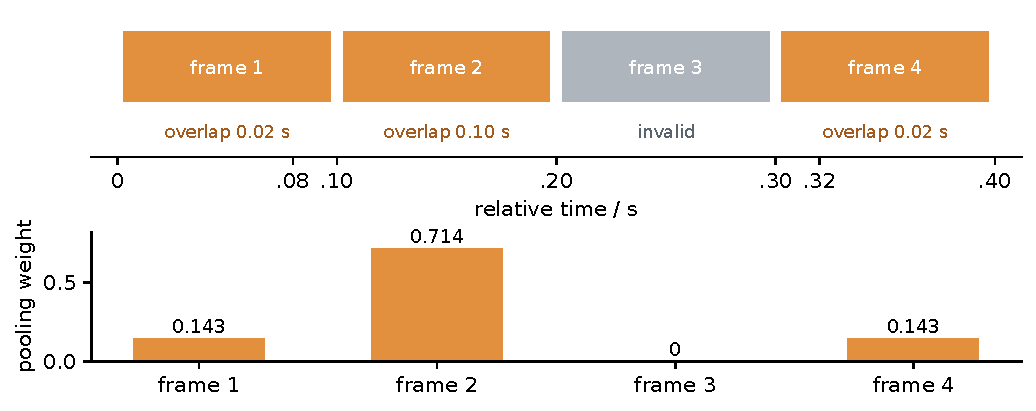
\includegraphics[width=0.92\linewidth]{figures/q1_overlap_example.pdf}
\caption{交叠池化示意算例。灰色第三帧的视觉特征无效，不进入加权平均；词锚点与有效帧的交叠决定权重，覆盖指标另外记录缺失程度。图中时间和权重为说明公式的构造值，并非附件1样本统计。}
\label{q1:fig:overlap}
\end{figure}

通过父词映射，将音视频词级特征复制到对应子词位置：
\begin{equation}
X^m_{ik}=\begin{cases}\bm x^m_{i,g_i(k)},&P_{ik}=1,\\\bm0,&P_{ik}=0,\end{cases}
\quad
O^m_{ik}=P_{ik}\ind\{d^m_{i,g_i(k)}>0\},\qquad m\in\{a,v\}.
\label{q1:eq:anchor}
\end{equation}
非内容位置的 $O$ 定义为0，不求值不存在的父词。三模态最终维度分别为
\begin{equation}
X^t_i\in\R^{50\times768},\qquad
X^a_i\in\R^{50\times25},\qquad
X^v_i\in\R^{50\times16}.
\end{equation}
多个子词继承父词的完整区间，不等分原词时间；$P=1,O^m=0$表示位置存在但该模态无观测，而不是一个真实的全零特征事件。

\paragraph{边界扰动与质量分量}

词边界变化会改变聚合帧及其权重。对区间两端加入标准差$s=40$\,ms的独立高斯扰动，采样$B=50$次并重新池化。两端先裁剪到模态时间范围；若终点不大于起点，设置20\,ms的最小区间。池化使用修正区间与有效帧的实际交叠，完全无覆盖的扰动另行计数。

令 $\mathcal H^m_{iu}$ 为有覆盖的扰动集合，$B^m_{iu}=|\mathcal H^m_{iu}|$。当 $B^m_{iu}\ge2$ 时定义
\begin{align}
\bar{\bm x}^{m,\mathrm{pert}}_{iu}&=\frac{1}{B^m_{iu}}\sum_{q\in\mathcal H^m_{iu}}\bm x^{m,(q)}_{iu},\\
V^m_{iu}&=\frac{1}{B^m_{iu}}\sum_{q\in\mathcal H^m_{iu}}
\left\|\bm x^{m,(q)}_{iu}-\bar{\bm x}^{m,\mathrm{pert}}_{iu}\right\|_2^2.
\label{q1:eq:variance}
\end{align}
原窗口无观测或有效扰动不足2次时，设置退化标记，方差字段以0占位。其余锚点的$V$衡量有观测条件下的边界敏感性，有效扰动次数$B^m_{iu}$随结果保存。

在每条样本内部，按有效帧计算模态尺度
\begin{equation}
\sigma_{im}^2=\frac{1}{N^{m,\mathrm{valid}}_i}\sum_{j:r^m_{ij}=1}
\|\bm f^m_{ij}-\bar{\bm f}^m_i\|_2^2+10^{-12},
\qquad \vt^m_{iu}=\frac{V^m_{iu}}{\max(\sigma_{im}^2,10^{-9})}.
\label{q1:eq:scale}
\end{equation}
少于2个有效帧时，尺度取1。归一化方差刻画池化变化相对于片段内特征变化的大小，各模态分别统计。

综合质量分数取
\begin{equation}
Q^m_{iu}=c_{iu}\,d^m_{iu}\exp(-\gamma_m\vt^m_{iu}),\qquad \gamma_a=\gamma_v=1.
\label{q1:eq:quality}
\end{equation}
路径置信度、观测覆盖和边界敏感性共同决定综合质量$Q$。保存$c,d,V,\vt,Q$及退化标记，可按质量排序定位待复核锚点，并追溯相应的影响分量。

三项分量相乘还有明确的边界行为：词对齐失败时没有可用锚点；锚点存在但人脸完全缺失时$d^v=0$，因而$Q^v=0$；仅当有覆盖且扰动能够产生至少两个有效池化结果时，边界敏感性才有可解释的估计。零覆盖与“稳定但数值小”属于不同状态，必须结合观测掩码和退化标记阅读$Q$。

\subsubsection{模型求解与参数设置}
\paragraph{求解流程}

在冻结预训练模型的条件下，按以下步骤求解特征与时间映射。

\begin{enumerate}
\item 读取样本标识与官方转写，建立原词字符区间及词元归属，生成文本特征和50位内容掩码。
\item 解码音轨，提取25维声学帧特征；对全量原词构建字符目标，计算CTC路径、词区间及路径置信度。
\item 按视频PTS读取帧，计算16维人脸特征及有效帧掩码，建立各帧支撑区间。
\item 对每个已生成区间的原词执行交叠池化和边界扰动；未生成区间的词保留失败记录，不赋予人为时间。
\item 将词级特征映射到保留的子词位置，输出特征、掩码和质量分量；保存全量词表及截断尾部记录。
\item 汇总100条样本，核查样本键、张量形状、区间顺序和有效范围，并生成全量清单与典型对应图。
\end{enumerate}

\paragraph{工具与关键参数}
扰动随机种子由样本标识的MD5摘要前8位生成，固定 $B,s,\gamma$ 后可在同一运行环境中复算。复现所需主要工具与参数见表\ref{q1:tab:environment}。

\begin{table}[htbp]
\centering\small
\caption{特征提取工具与关键参数}
\label{q1:tab:environment}
\begin{tabularx}{\linewidth}{p{2.3cm}p{4.4cm}Y}
\toprule
模块 & 工具及版本 & 设置 \\
\midrule
运行环境 & Python 3.12.10，CPU & NumPy 1.26.4，pandas 2.3.3 \\
音视频解码 & PyAV 18.1.0 & 音频16\,kHz单声道，视觉采用解码PTS \\
文本编码 & transformers 4.56.0 & \file{bert-base-uncased}，推理模式，50位 \\
声学描述符 & openSMILE 2.6.0 & eGeMAPSv02，LLD层，25维 \\
词级对齐 & torch / torchaudio 2.8.0 & \file{WAV2VEC2\_ASR\_BASE\_960H}，20\,ms帧移 \\
人脸描述符 & MediaPipe 0.10.21 & FaceDetection与FaceMesh，478点，ROI倍率1.6 \\
边界扰动 & NumPy随机生成器 & $B=50$，$s=40$\,ms，$\gamma_a=\gamma_v=1$ \\
\bottomrule
\end{tabularx}
\end{table}

逐样本运行记录的累计处理耗时为9.43\,min，平均每条5.66\,s。其中视觉处理482.20\,s，占85.3\%；文本、音频及池化阶段分别为6.95、65.16和11.25\,s。该统计来自逐样本日志，不包含首次下载模型、论文绘图与编译，实际复现耗时随硬件和缓存状态变化。

特征张量、词级时间与帧级记录通过样本键和父词索引关联，形成表\ref{q1:tab:checklist}所示的数据组织。文件字段、读取示例和100条逐项结果见附录\ref{app:q1-files}。
\begin{table}[htbp]
\centering\small
\caption{多模态特征的层次组织与追溯关系}
\label{q1:tab:checklist}
\begin{tabularx}{\linewidth}{p{2.2cm}Y}
\toprule
核验对象 & 输出记录与全量结果 \\
\midrule
样本对应 & 以唯一样本键连接媒体、转写和输出，清单保存输入哈希；100条输入均对应特征记录 \\
序列组织 & 固定50位，三模态维度为768/25/16；保存内容掩码$P$、父词索引$U$及观测掩码$O^a/O^v$ \\
时间追溯 & 1932条原词明细中1920条有区间$[a,b)$；帧级文件保存音频支撑区间、视频PTS及有效标记 \\
可复现性 & 保存工具版本、参数、逐样本耗时和随机种子规则；保留100份逐样本记录与100份帧级文件 \\
\bottomrule
\end{tabularx}
\end{table}

\subsubsection{实验结果与分析}
\label{q1:sec:results}

\paragraph{全量处理结果与统计口径}

100条样本均完成处理。1932个原词中，1920个生成时间区间，区间生成率为99.38\%；其余12项包括6个数字词和6个标点或符号串，均未通过字符目标构造。已生成区间全部满足非负起点、正长度、音轨范围内终点和起点随词序单调四项条件。

\begin{table}[htbp]
\centering\small
\caption{全量特征生成与覆盖结果}
\label{q1:tab:overall}
\begin{tabularx}{\linewidth}{p{5.3cm}p{3.4cm}Y}
\toprule
指标 & 结果 & 统计范围 \\
\midrule
样本输出 / 原词记录 & 100 / 1932 & 附件1全量 \\
生成区间的原词 & 1920（99.38\%） & 全部1932词 \\
词区间时长均值 / 中位数 & 0.219 / 0.160\,s & 1920个已生成区间 \\
路径置信度均值 / 中位数 & 0.750 / 0.969 & 同上 \\
音频覆盖均值 & 1.000 / 0.9938 & 已生成区间 / 全部原词 \\
视觉覆盖均值 & 0.9302 / 0.9245 & 已生成区间 / 全部原词 \\
视觉零覆盖词数 & 120 / 132 & 已生成区间 / 全部原词 \\
全片未检出人脸的样本 & 4 & 100条样本 \\
触发截断的样本 & 6 & 100条样本 \\
未进入接口的词元 / 完全失位原词 & 70 / 52 & 全量文本尾部记录 \\
\bottomrule
\end{tabularx}
\end{table}

表\ref{q1:tab:overall}以全部1932个原词与已生成区间的1920个原词为两个统计范围。音频覆盖在已生成区间上达到1.000，视觉覆盖均值仅0.9302，说明锚点信息的不完整主要来自人脸观测，而非声学支撑。

12个未生成区间的词在固定接口中仍占22个内容位置，其内容掩码$P=1$，观测掩码$O^a=O^v=0$。三态表示由此可以区分“有文本、无时间支撑”与“文本、时间支撑齐备”两类位置。另有120个已生成区间的词缺少视觉覆盖，说明时间区间是否有效与人脸观测是否有效是两个独立条件。

已生成区间的词时长中位数为0.160\,s，其中28.1\%短于0.10\,s；若以解码音频总时长777.0091\,s除以1932个原词，含词间停顿的平均间隔约为0.402\,s。两者的差异说明：按词数均分音轨会把词间停顿摊入相邻词，并掩盖短词的真实边界。CTC区间与交叠池化因此分别在声学证据与实际帧支撑上计算，而不由总时长反推每词边界。


图\ref{q1:fig:coverage-summary}从词元长度与词级观测状态解释接口覆盖的构成。全量2317个内容词元中，2247个进入固定接口，保留比例为96.98\%；音频零覆盖的12词均未生成时间区间。视觉方面，除这12词外，还有120个已生成区间的词没有有效人脸特征支撑。因此，时间锚点的存在与模态观测的存在是两个独立条件，在模型中分别由内容掩码$P$与观测掩码$O^m$表达。
\begin{figure}[htbp]
\centering
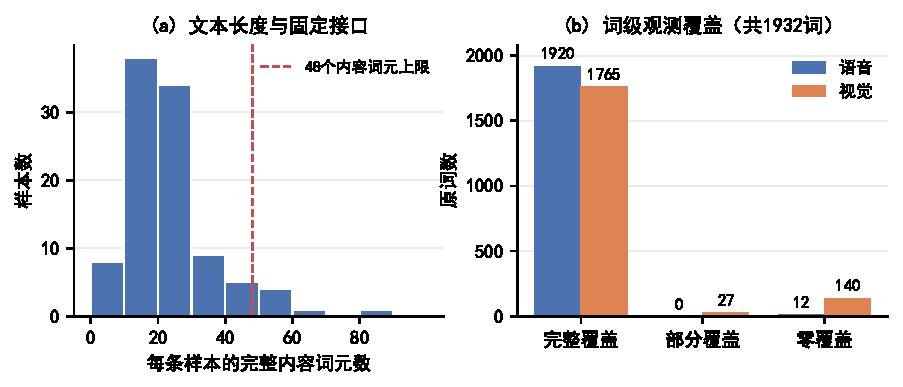
\includegraphics[width=\linewidth]{figures/q1_coverage_summary.pdf}
\caption{由样本清单和词级明细重算的接口覆盖情况。左图为100条样本的完整词元数，虚线表示48个内容词元上限；6条样本触发截断，共70个词元未进入接口。右图以全部1932个原词为分母，区分完整、部分与零覆盖；完整覆盖按$d\geq1-10^{-6}$判定。}
\label{q1:fig:coverage-summary}
\end{figure}

\paragraph{典型样本的文本、语音与视频对应}

选取样本\file{-I\_e4mIh0yE\$\_\$1}。图\ref{q1:fig:typical}在统一秒轴上展示6个原词的音频区间、区间附近的视频帧，以及对应声学与视觉特征；表\ref{q1:tab:typical}给出数值关系。文本向量由这些词对应的BERT内容位置取得，视频帧则通过PTS定位，不由50位下标换算时间。

\begin{figure}[htbp]
\centering
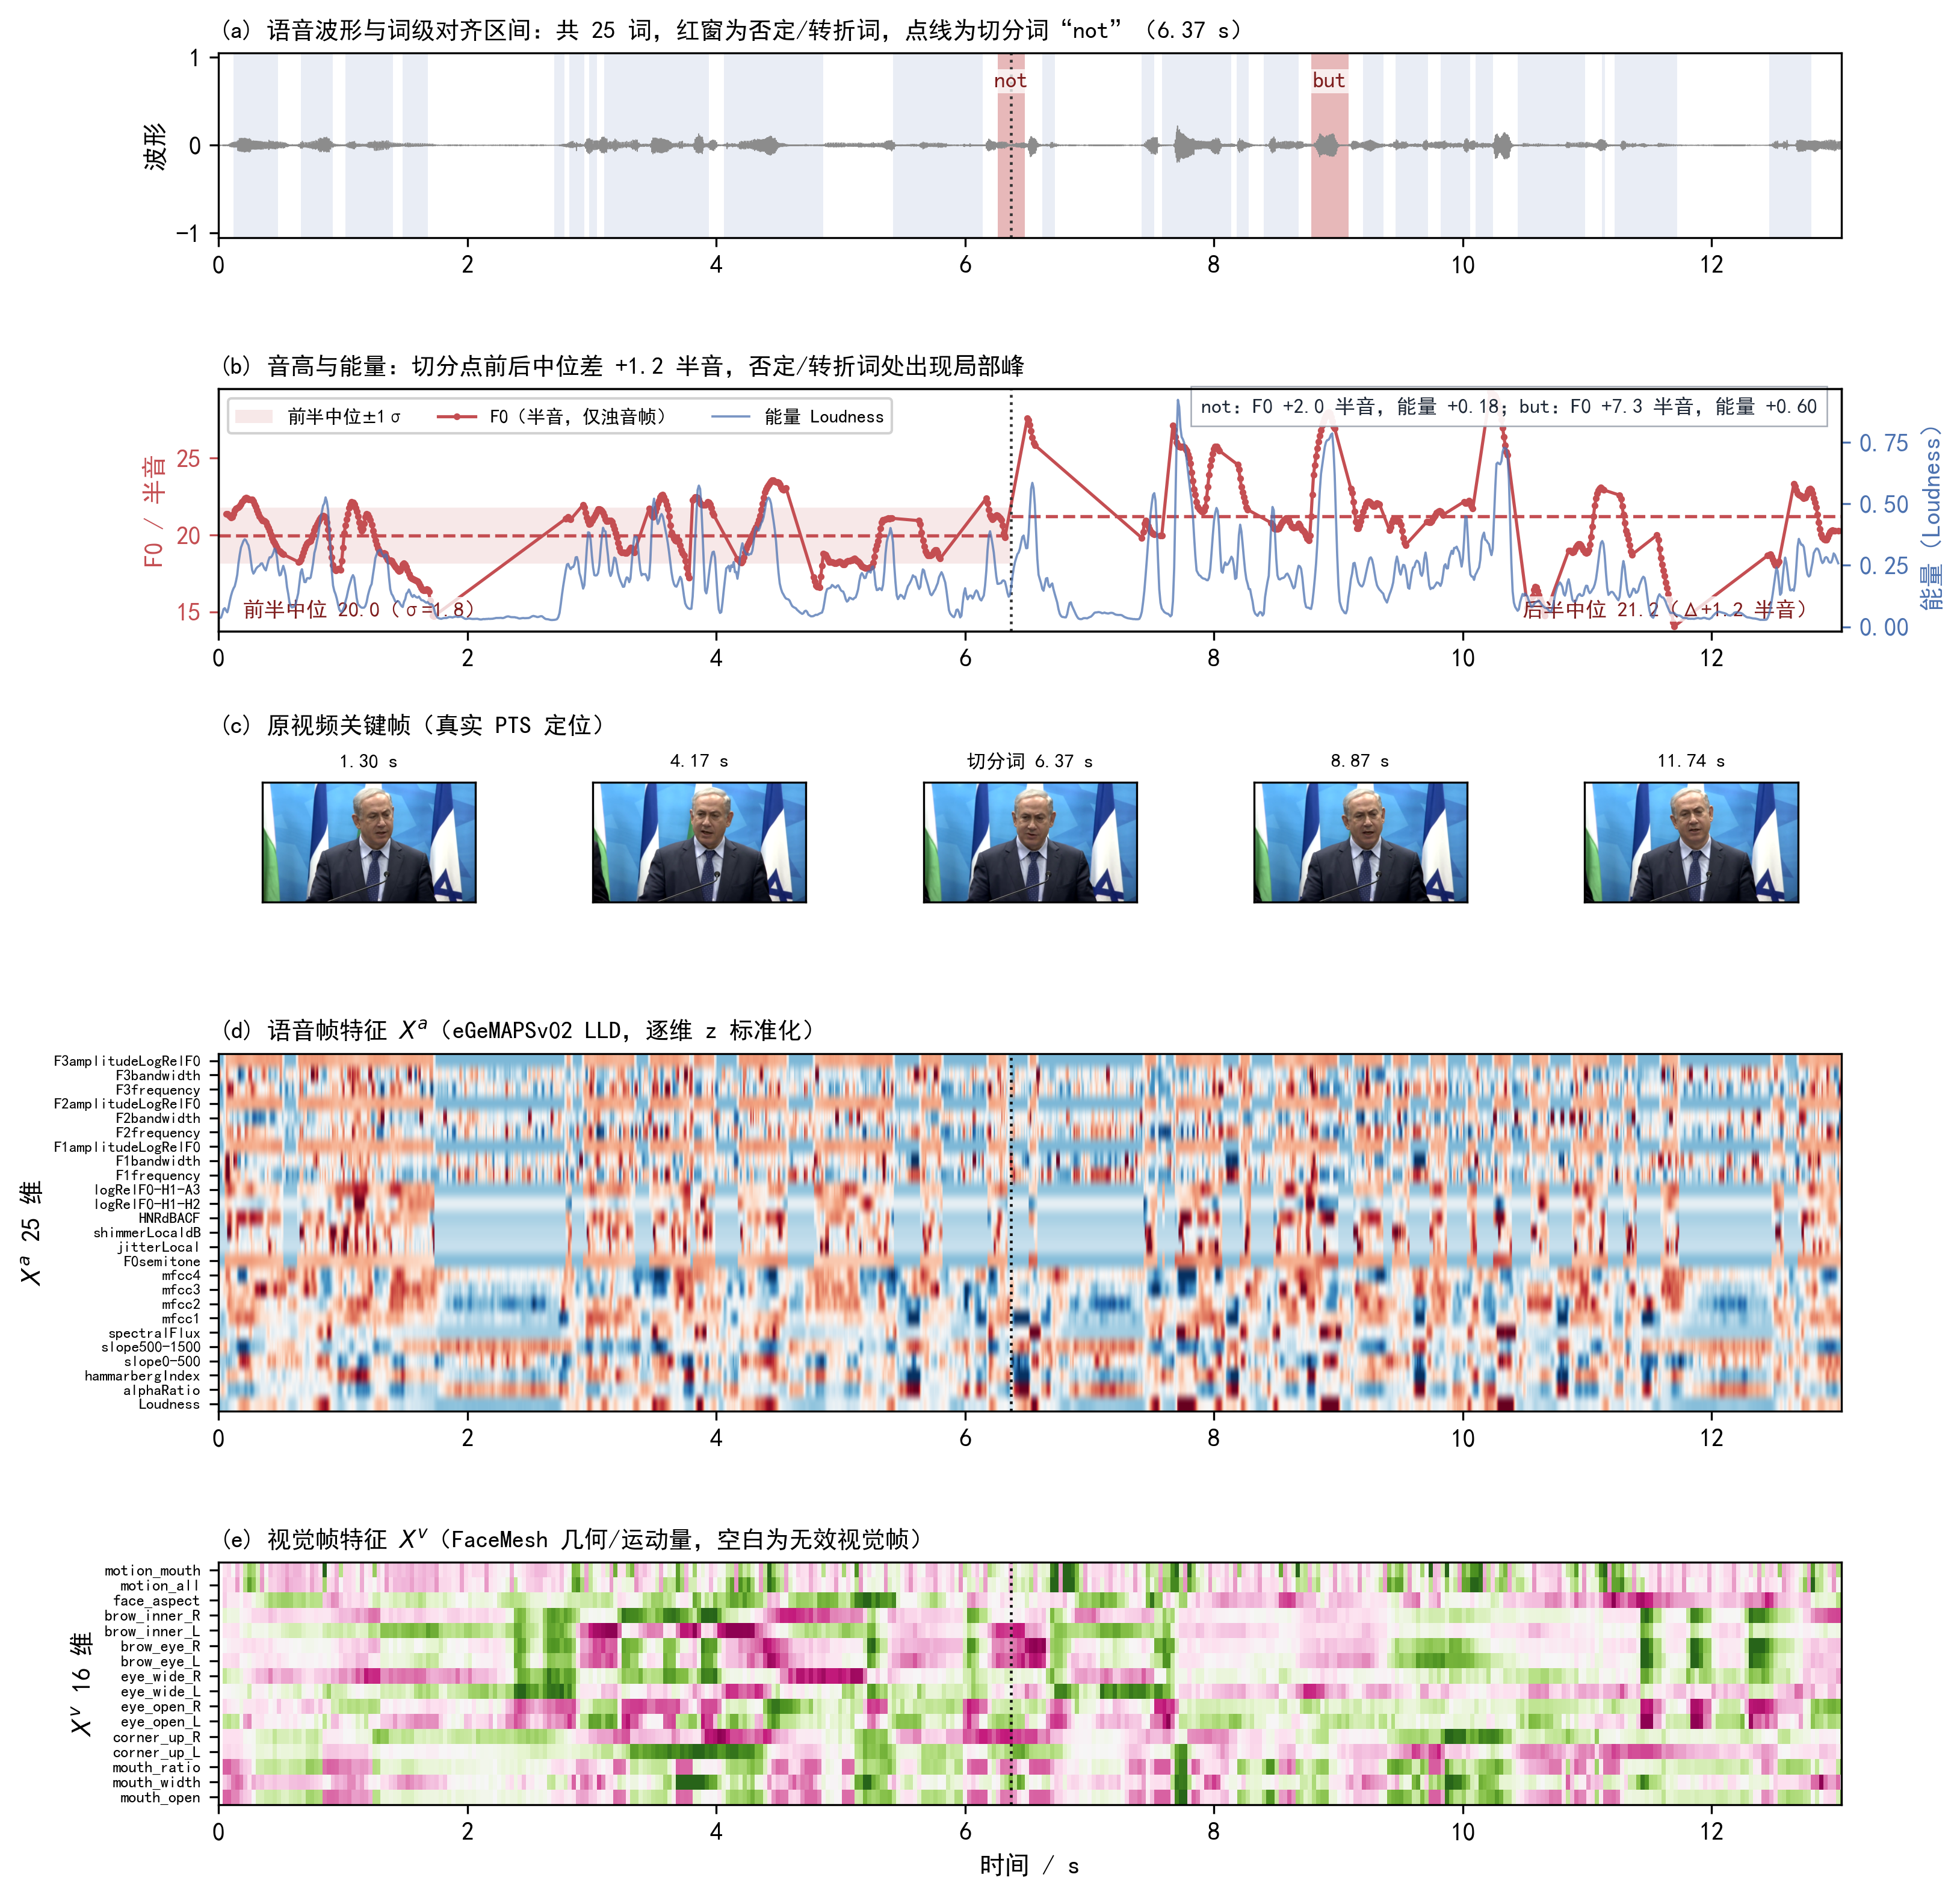
\includegraphics[width=\linewidth]{figures/q1_fig8_typical_correspondence.png}
\caption{典型样本的原词、音频区间、视频帧和帧级特征对应。标出的6个原词依次关联其音频窗口和视频画面；声学热图的逐维标准化仅用于可视化。}
\label{q1:fig:typical}
\end{figure}
\begin{table}[htbp]
\centering\small
\caption{典型样本的词区间与三模态映射。每个内容词元对应768维文本向量，并继承父词的25维语音向量与16维视觉向量。}
\label{q1:tab:typical}
\begin{tabular}{lccccc}
\toprule
原词 & 语音区间(s) & 内容词元数 & $c$ & $d^a$ & $d^v$ \\
\midrule
\texttt{States} & [1.34, 1.58) & 1 & 0.999 & 1.00 & 1.00 \\
\texttt{punish} & [2.20, 2.50) & 1 & 0.965 & 1.00 & 1.00 \\
\texttt{to} & [3.52, 3.62) & 1 & 1.000 & 1.00 & 1.00 \\
\texttt{which} & [4.42, 4.62) & 1 & 1.000 & 1.00 & 1.00 \\
\texttt{punished} & [5.50, 5.86) & 1 & 0.960 & 1.00 & 1.00 \\
\texttt{Europe.} & [6.62, 6.86) & 2 & 0.964 & 1.00 & 1.00 \\
\bottomrule
\end{tabular}
\end{table}

以\file{Europe.}为例，父词区间为$[6.62,6.86)$\,s，两个词元共享该区间，分别对应768维上下文文本表示，并继承相同的音视频池化向量。由此，词元语义、语音窗口和视频帧段通过父词区间建立一致的对应关系。

\paragraph{观测缺失与截断的处理效果}

图\ref{q1:fig:missing}展示人脸检出率为37.5\%的样本\file{-HwX2H8Z4hY\$\_\$5}。无有效视觉支撑的锚点取$O^v=0$、$Q^v=0$，其余位置按有效帧池化；音频与文本保留各自可用信息。该例说明位置级掩码能够刻画同一样本内部的局部模态缺失。

\begin{figure}[htbp]
\centering
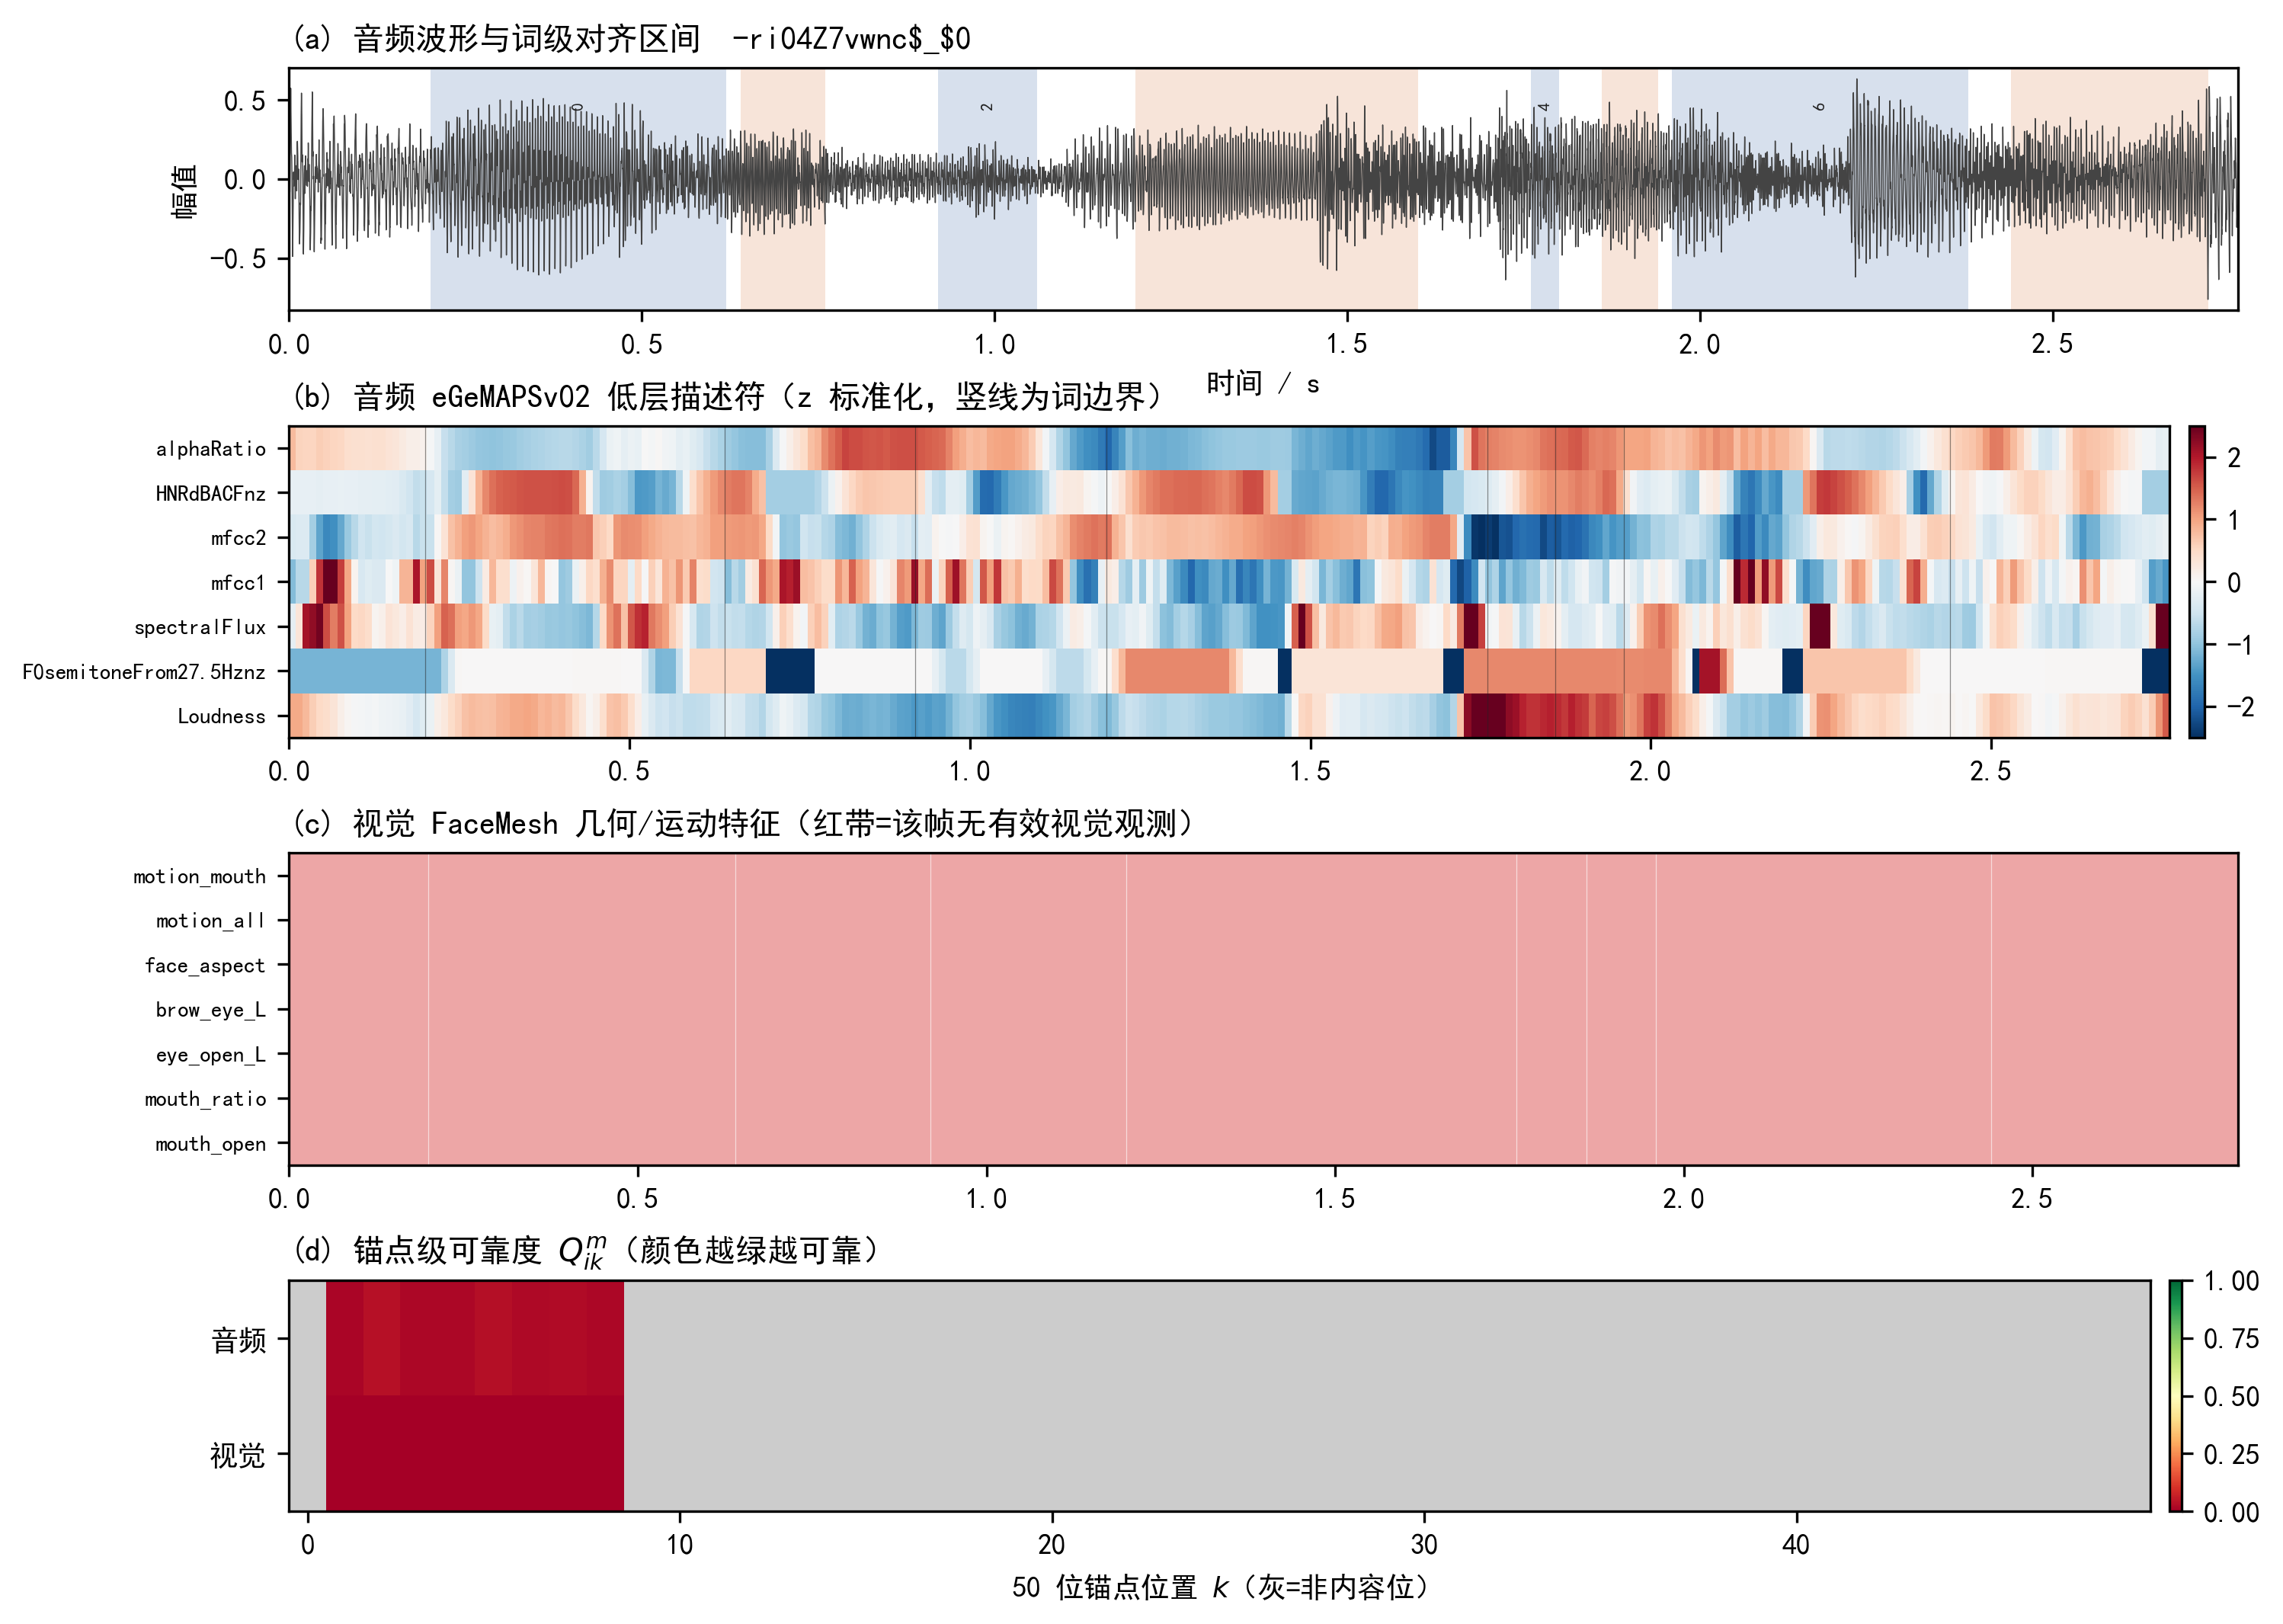
\includegraphics[width=0.91\linewidth]{figures/q1_fig1_overview_missing.png}
\caption{局部视觉观测缺失样本。上三幅以秒为横轴，下方质量条带以50位接口索引为横轴，二者通过父词映射和词区间关联。红带表示人脸特征无有效观测，灰色接口位置为非内容位。}
\label{q1:fig:missing}
\end{figure}

文本方面，6条样本超过48个内容词元，合计70个词元未进入接口，52个原词完全失去接口位置。最严重样本含65个原词、82个词元，其中34个词元与26个原词位于接口之外；这些词元的词级时间与音视频记录仍保留于全量输出。接口长度属于可配置参数，扩展后即可在相同记录上重新编码，无需重复特征提取。

图\ref{q1:fig:truncation}并列展示定长接口与全量词区间。蓝色部分对应保留的48个内容词元，红色三格示意截断尾部；中图展示65个原词的时间记录，由此区分位置级输出范围与全量时间记录范围。
\begin{figure}[htbp]
\centering
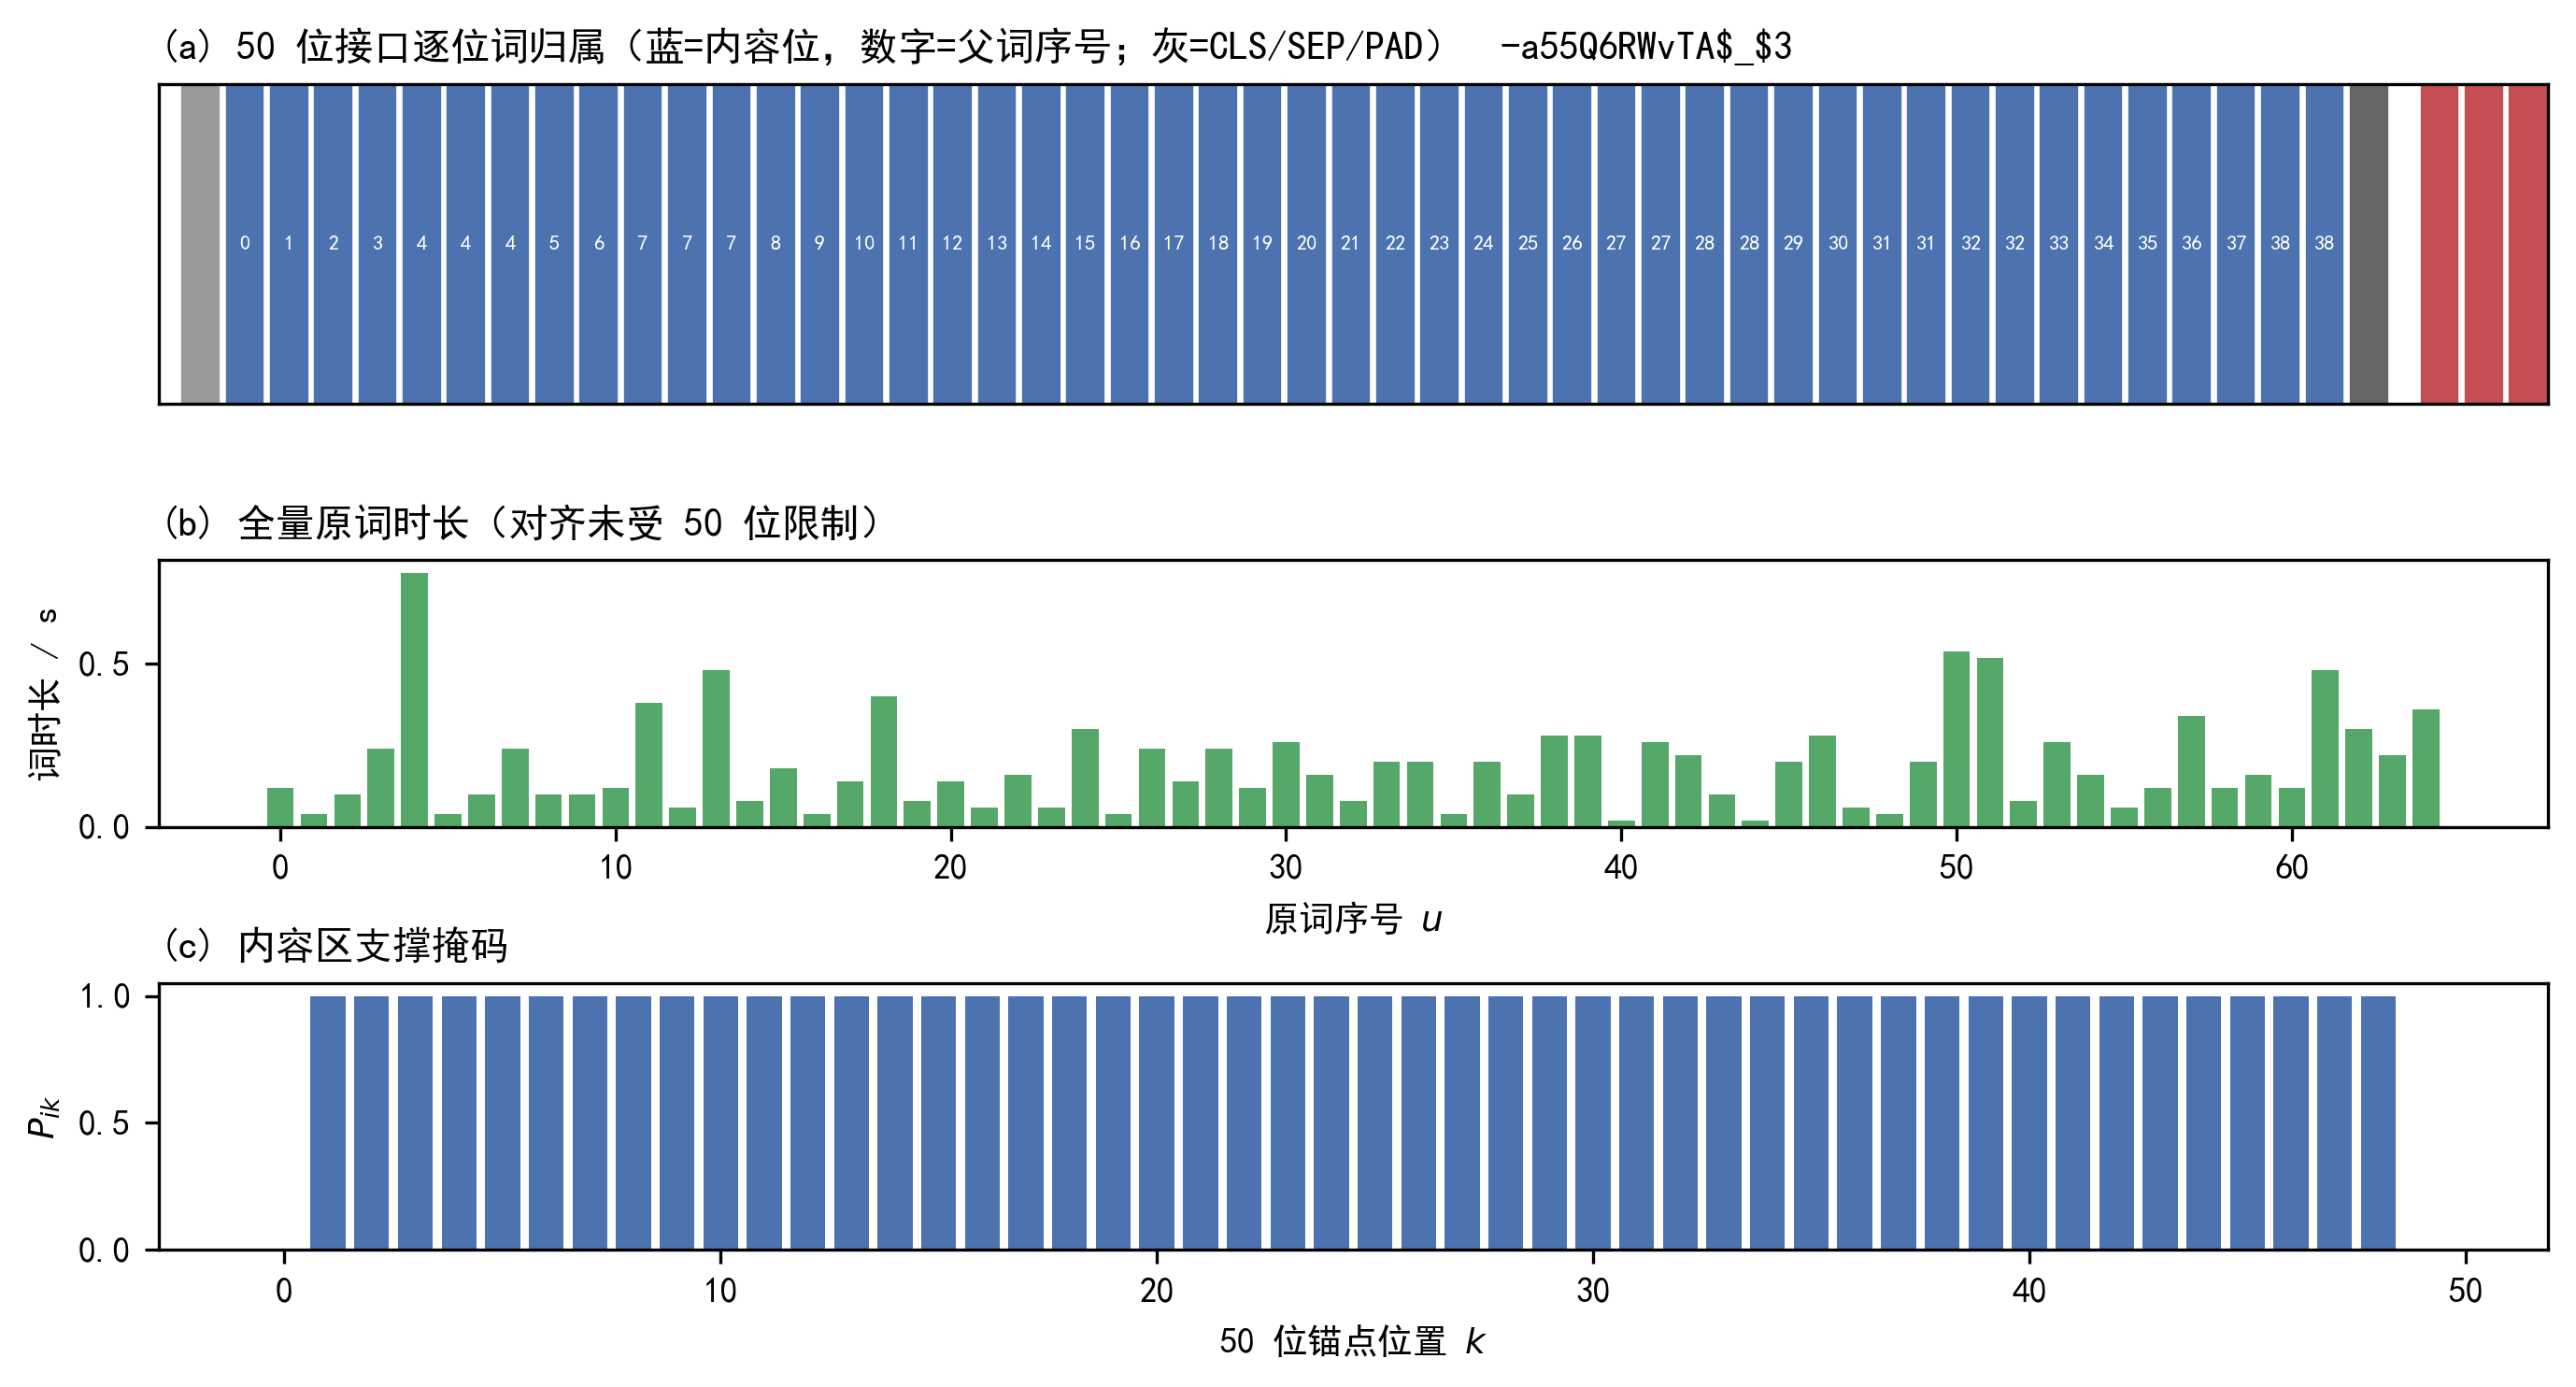
\includegraphics[width=\linewidth]{figures/q1_truncation.png}
\caption{样本\file{-a55Q6RWvTA\$\_\$3}的文本接口截断。上：50位接口的词元归属，右侧红格为截断尾部示意；中：全部原词的时间区间；下：内容掩码。实际有34个尾部词元未形成位置级文本特征，但词级时间记录仍保留。}
\label{q1:fig:truncation}
\end{figure}

\paragraph{质量分量与参数敏感性}

\begin{table}[htbp]
\centering\small
\caption{质量分量统计（1920个已生成时间区间的原词）}
\label{q1:tab:quality}
\begin{tabular}{lrrrr}
\toprule
分量 & 音频均值 & 音频中位数 & 视觉均值 & 视觉中位数 \\
\midrule
覆盖指标 $d$ & 1.0000 & 1.0000 & 0.9302 & 1.0000 \\
归一化扰动方差 $\vt$ & 0.0931 & 0.0471 & 0.0498 & 0.0186 \\
综合质量 $Q$ & 0.6848 & 0.8673 & 0.6904 & 0.9128 \\
\bottomrule
\end{tabular}
\end{table}

音频与视觉$\vt$的95\%分位数分别为0.3328和0.1875，120个视觉零覆盖词另记为退化状态。音视频$Q$的Spearman相关约为0.765：两者共享路径置信度因子，排序差异则来自各自独立的覆盖与扰动分量。

图\ref{q1:fig:quality}展示质量分量及音视频$Q$的联合分布。路径置信度的差异使相同覆盖率的锚点具有不同质量；视觉$Q=0$对应零覆盖词。归一化扰动方差采用对数坐标展示，退化记录通过独立标记识别。
\begin{figure}[htbp]
\centering
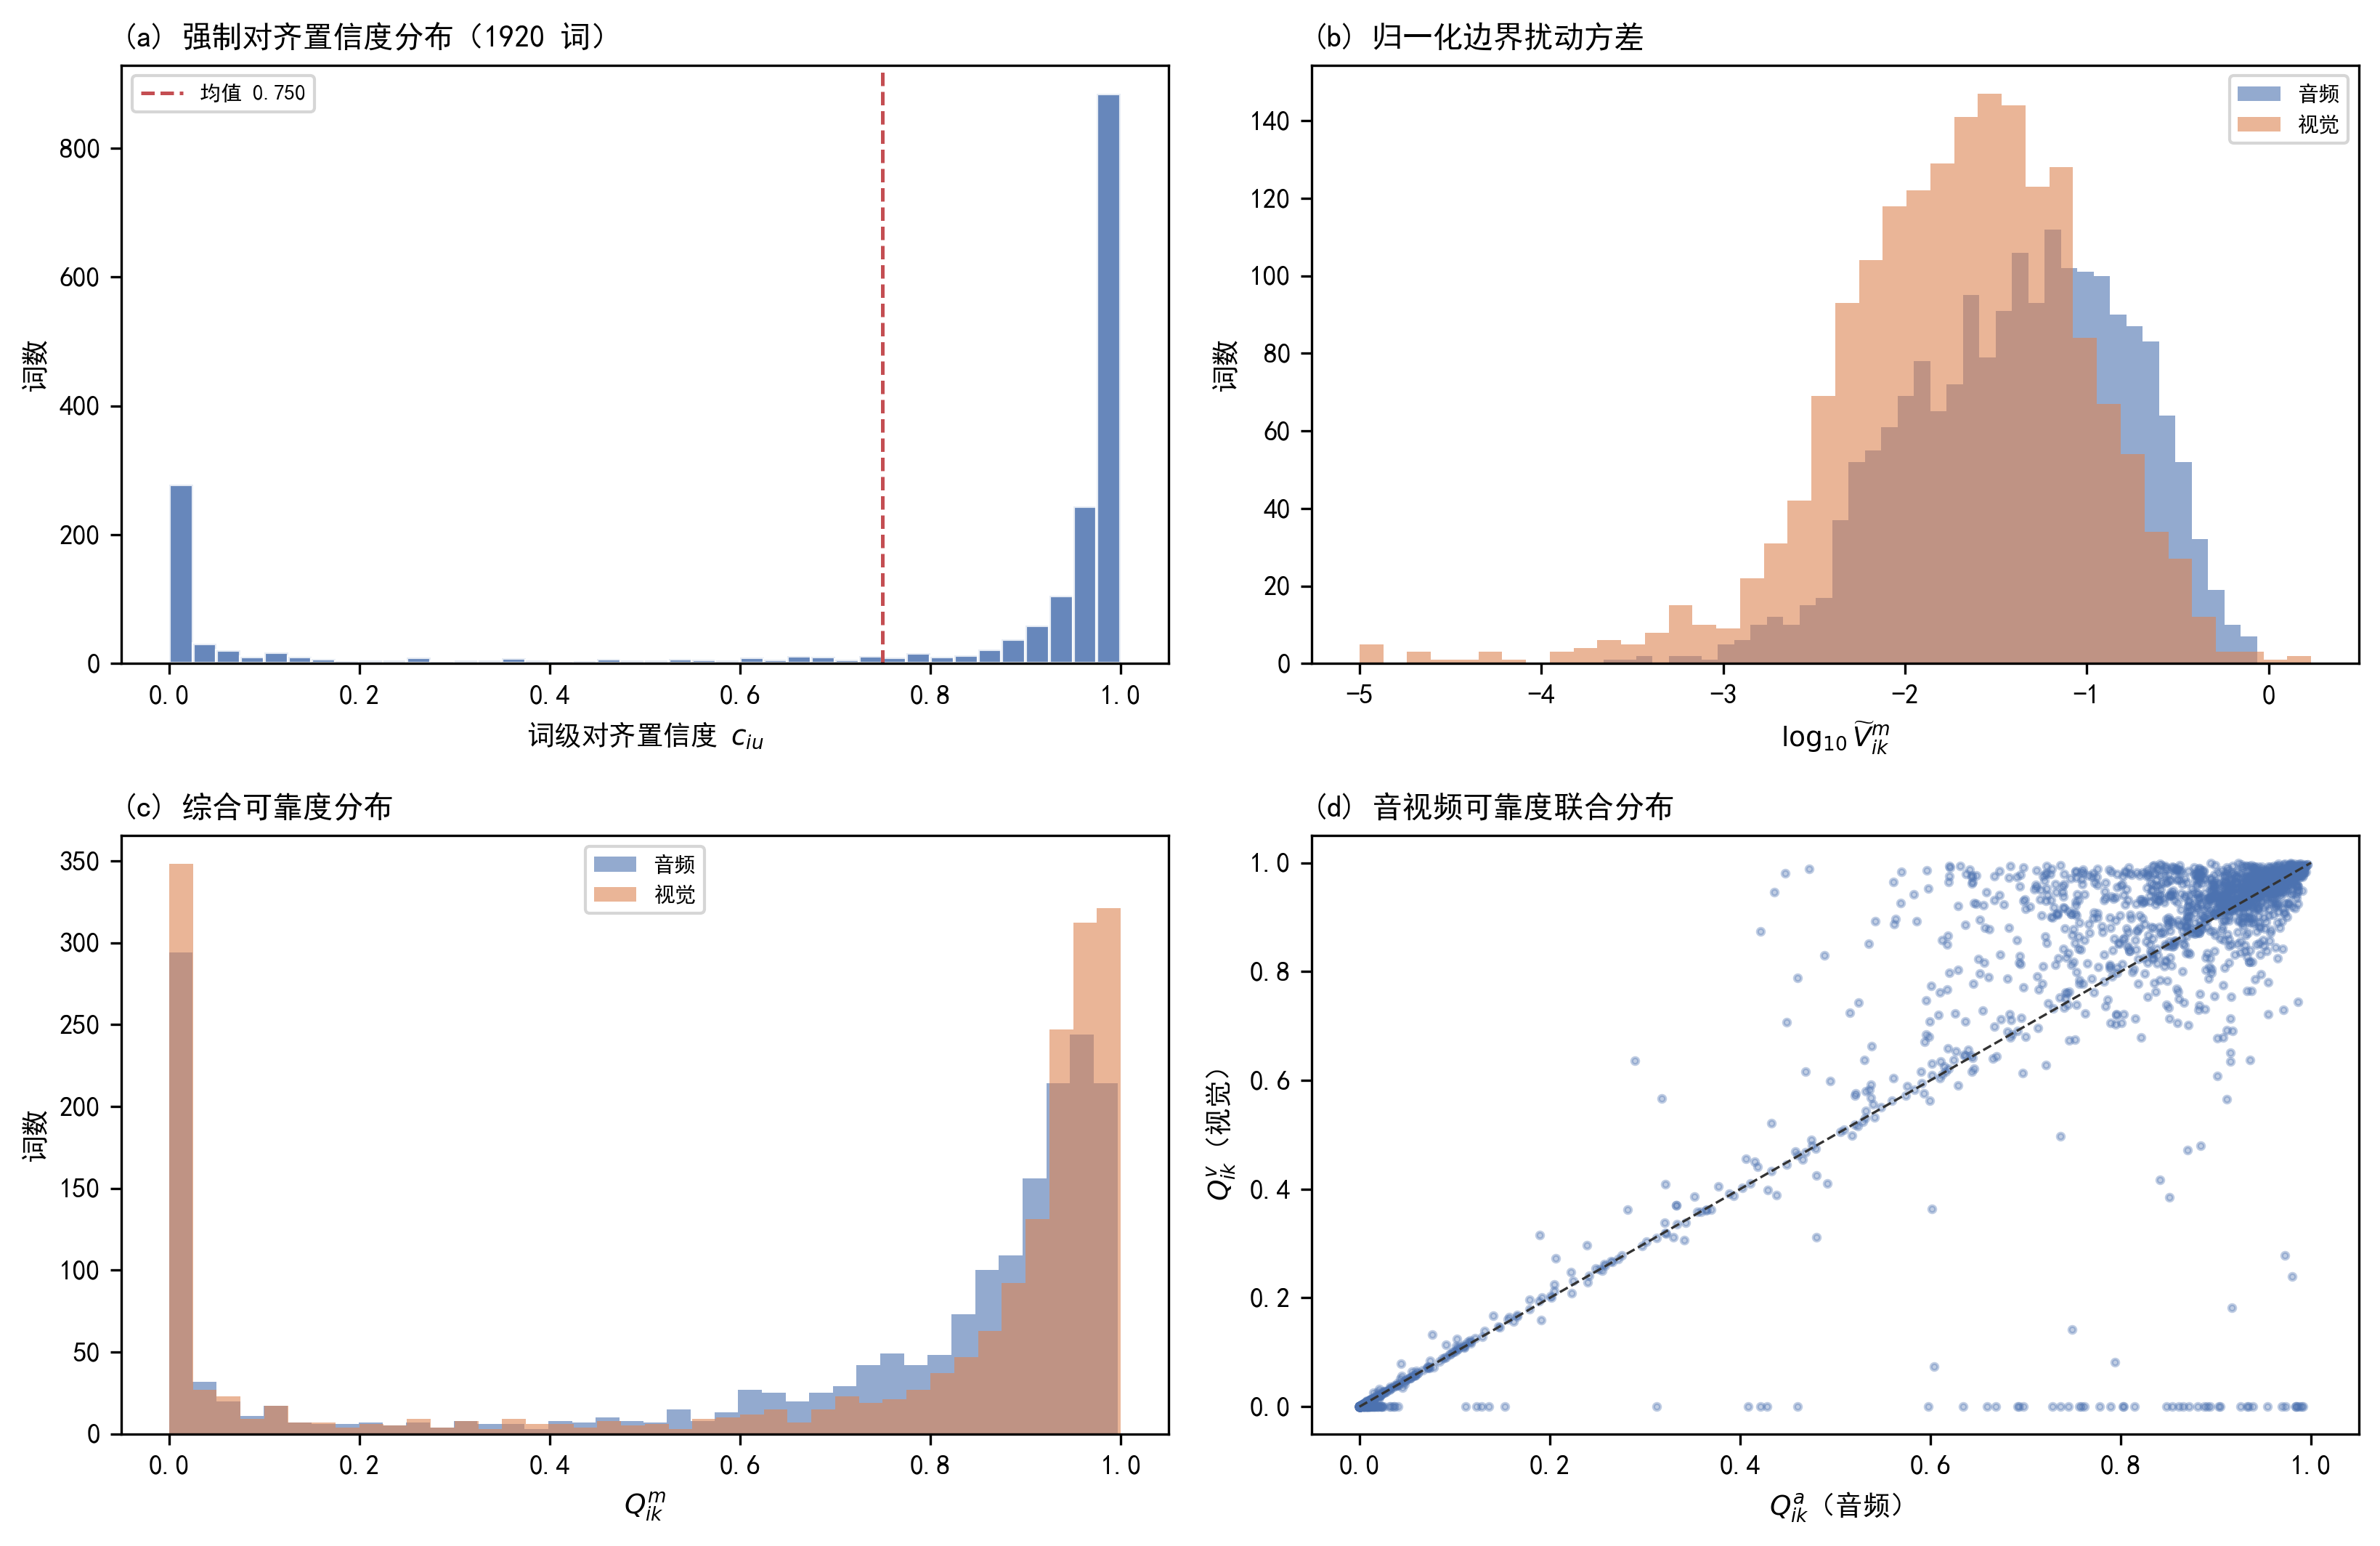
\includegraphics[width=\linewidth]{figures/q1_quality.png}
\caption{1920个已生成词区间的路径置信度、归一化边界扰动方差和综合质量分布。图(d)的音视频质量相关包含共享的路径置信度因子；零覆盖与退化记录需结合掩码判断。}
\label{q1:fig:quality}
\end{figure}

质量分数的三个参数按词区间的时间尺度与模块规模设定：衰减系数$\gamma$控制覆盖偏离的惩罚强度，扰动次数$B$与尺度$s$决定边界敏感性的估计精度。表\ref{q1:tab:sensitivity}给出三者变化时的排序一致性，用以检验质量分量的取值是否依赖具体参数设定。

\begin{table}[htbp]
\centering\small
\caption{参数敏感性结果与适用范围}
\label{q1:tab:sensitivity}
\begin{tabularx}{\linewidth}{p{2.1cm}p{4.8cm}Y}
\toprule
实验 & 已有结果 & 适用范围 \\
\midrule
$\gamma$变化 & 音频 $Q$：0.5和2相对1的样本内排序相关均值0.974、0.972 & 音频质量分量的排序在该参数取值范围内保持稳定 \\
$B$变化 & 视觉 $V$：50相对200的排序相关0.995 & 在排序前12条样本各前8词上核算的视觉方差排序 \\
$s$变化 & 相对40\,ms，20\,ms的样本内 $Q$ 排序相关均值0.937/0.937，80\,ms为0.960/0.901 & 音频与视觉分别计算的样本内排序一致性 \\
\bottomrule
\end{tabularx}
\end{table}

在所选子集上，$B=50$与200的视觉方差排序相关为0.995，两种扰动次数对锚点给出的排序高度一致；22.9\%的点值平均差则来自扰动采样的随机波动。质量分量的排序结构不随扰动次数的具体取值改变，可用于锚点间的相对比较。

\paragraph{相对时序一致性检验}

若时间映射正确，人为错位应当降低音视频之间的词级关联。据此设计单模态错位实验：保持一侧词窗口不动，仅将另一侧平移$\pm0.25$、$\pm0.5$或$\pm1.0$\,s，比较响度与嘴部开合、嘴部运动的词级相关。12种非零错位条件下的两项平均相关均低于各自的样本配对基线，24项Wilcoxon检验中20项在未校正的5\%水平上显著，最小$p$约为$2.20\times10^{-8}$。

各错位条件分别剔除越界与无覆盖词，相关变化同时包含时间平移与可用词集合变化的影响。在该口径下，任一非零错位都使两项相关下降，且多数差异在统计上显著，说明当前时间映射保持了音视频之间的词级关联。

在83条人脸检出率较高的样本上，包络相关最大值对应的延迟中位数为嘴部开合$+0.09$\,s、嘴部运动$+0.22$\,s与全脸运动$+0.27$\,s，正值表示音频包络较晚。该量记为\textbf{包络最佳延迟}，用于描述词级音视频的联动强度，其取值依赖特征类型、取样方式与搜索范围。

附录\ref{app:q1-files}列出特征文件字段、读取方法及附件1全部100条样本的结果，与本节汇总统计和典型样本共同呈现特征生成、时间映射及观测覆盖情况。

\paragraph{结果讨论与适用范围}

本模型把“三模态特征的组织”与“原始时间对应”作为两个问题分别处理，以词级区间作为可解释的中间变量：字符偏移保证子词归属可追踪，时间交叠池化使不同采样频率的特征映射到同一锚点，内容掩码与观测掩码分别刻画接口结构与模态可用性，三者共同构成该问的证据链。

本问的验证覆盖样本完整性、时间区间结构、观测覆盖与典型片段对应关系：99.38\%的词区间生成率与典型样本的逐项对应共同支持处理流程的可追溯性，质量分量则在给定的提取与扰动规则下区分锚点的可用程度。50位接口之外的词级时间与音视频记录保留于完整输出，位置级文本表示覆盖前48个内容词元。

据此获得附件1全部100条样本的三模态特征，输出维度为$50\times768$、$50\times25$与$50\times16$，1932条原词记录中1920条生成时间区间。典型样本给出了文本、语音与视频的对应过程，全量结果及文件规范见附录\ref{app:q1-files}。

\FloatBarrier


\subsection{问题二的模型建立与求解}
\label{sec:q2}

\subsubsection{问题分析与建模思路}
实际交互中的转写失败、语音中断和画面遮挡，通常只使某一模态的局部连续片段不可用。问题二要求在此条件下，同时预测样本的情感极性与连续情感强度，并分析缺失模态、缺失位置、缺口长度及缺失率对预测性能的影响。因此，建模的关键不仅是融合三类特征，还在于区分有效观测与缺失信息，并控制不可靠补全对最终判断的影响。

针对上述问题，构建三态感知可靠补全与融合网络TSRF-D，并采用教师--学生任务蒸馏进行训练。模型以结构填充、有效观测和局部缺失三种状态描述输入，利用样本内可用节点生成补全表示，通过可靠度门控调节补全信息与缺失嵌入的融合比例。在此基础上，采用双向时序编码器提取序列特征，实现情感极性与强度的联合预测。教师基于原始可用输入学习情感分布，学生在局部遮挡输入下同时接受标签监督和教师软监督。

问题一研究原始素材的特征提取与时间对齐，本问研究对齐特征在局部缺失条件下的情感预测。根据赛题数据安排，训练与评价采用附件2的对齐版特征，专项推理采用附件3的对应版本。两问沿用一致的时序表示思想，各自使用相应附件的特征维度与输入接口。

\subsubsection{数据准备}
\paragraph{数据划分与输入接口}
附件2共含4850条样本，按题目给定划分使用3395条训练样本、728条验证样本和727条测试样本；附件3包含30条无标签样本。每个样本存储为至多50个对齐序列位置，文本、语音、视觉特征维度分别为768、74和35。三分类标签对应负向、中性和正向，连续强度位于$[-3,3]$；其中0仅属于中性类。强度标签包含非整数值，故按连续回归处理。

为统一训练与专项推理的文本输入，采用冻结的\file{bert-base-uncased}第12层，将\file{text\_bert}中的词元编号、注意力掩码和分段编号转换为连续表示。重算特征与附件2自带特征的平均绝对偏差约为$6.6\times10^{-7}$，最小余弦相似度约为0.9999997，二者具有较高的数值一致性。

本文以对齐锚点为时间组织单位，假设同一锚点上的三模态特征具有附件规定的时间对应关系。由于附件2未提供逐词时间戳，缺口长度统一以锚点数度量。声学与视觉向量作为整体特征参与建模。

\begin{table}[htbp]\centering\small
\caption{数据接口与处理约定}\label{q2:tab:data}
\begin{tabularx}{\linewidth}{p{2.4cm}Y Y}\toprule
项目 & 附件2 & 附件3\\\midrule
用途与规模 & 训练3395、验证728、测试727 & 最终预测30条，无标签\\
输入形状 & \multicolumn{2}{l}{$X^t\in\R^{50\times768}$，$X^a\in\R^{50\times74}$，$X^v\in\R^{50\times35}$}\\
文本入口 & \multicolumn{2}{l}{使用相同冻结BERT，由\file{text\_bert}生成连续表示}\\
缺失识别 & \multicolumn{2}{l}{文本内容位的\file{[UNK]}；语音、视觉内容位的全零向量}\\
统计量估计 & 仅训练集观测位置估计均值与标准差 & 复用训练统计量\\
评价方式 & 基于真实标签计算分类与回归指标 & 汇总全量预测及预测概率分布\\\bottomrule
\end{tabularx}\end{table}

\paragraph{内容、观测与人工缺失掩码}
记样本为$i$，锚点为$k$，模态$m\in\{t,a,v\}$。内容掩码$P_{ik}$由注意力有效位排除\file{[CLS]}和\file{[SEP]}得到。自然观测掩码分别定义为
\begin{align}
 O^t_{ik}&=P_{ik}\ind\{\mathrm{token}_{ik}\ne[\mathrm{UNK}]\},\\
 O^a_{ik}&=P_{ik}\ind\{X^a_{ik}\ne\bm0\},\qquad
 O^v_{ik}=P_{ik}\ind\{X^v_{ik}\ne\bm0\}.
\end{align}
其中$X^m_{ik}\ne\bm0$表示该向量至少有一个非零分量。依据附件的缺失标记规则，文本由词元标记识别缺失，语音和视觉由全零向量识别缺失，三路观测掩码分别计算。

令人工遮挡掩码为$H^m_{ik}$，且$H^m_{ik}\le O^m_{ik}$，则最终观测掩码$\widetilde O^m_{ik}=O^m_{ik}(1-H^m_{ik})$。三态变量定义为
\begin{equation}
s^m_{ik}=\begin{cases}
0,&P_{ik}=0,\\1,&P_{ik}=1,\ \widetilde O^m_{ik}=1,\\2,&P_{ik}=1,\ \widetilde O^m_{ik}=0.
\end{cases}
\end{equation}
自然缺失与人工缺失在模型输入中均为状态2，但仅人工遮挡位置保留可用于重建评价的原始真值。对模态$m$的第$j$维，使用训练集观测位置估计$\mu^m_j,\sigma^m_j$并计算
\begin{equation}
\bar X^m_{ikj}=\frac{X^m_{ikj}-\mu^m_j}{\widetilde\sigma^m_j},\qquad
\widetilde\sigma^m_j=\begin{cases}1,&\sigma^m_j<10^{-6},\\\sigma^m_j,&\text{其他}.
\end{cases}
\end{equation}
结构位在标准化后置零，缺失位通过观测掩码排除于候选集合之外。人工音视频遮挡使用标准化空间中的零值；文本则\textbf{先将选定词元替换为\file{[UNK]}，再经BERT编码}，同时保留原有序列位置。这样可以避免未遮挡位置的上下文表示提前包含已删除文本信息。

附件3共含605个内容锚点，文本、语音和视觉分别有131、131和135个缺失位置。文本与语音掩码在30条样本上逐位一致，文本与视觉掩码在29条样本上逐位一致，缺失主要表现为多模态局部同段共缺。

\subsubsection{模型构建}
\paragraph{总体结构与三态投影}
图\ref{q2:fig:arch}给出学生网络及教师监督的关系。学生的计算顺序为投影、补全与门控、时序编码、池化和双任务预测；时序编码位于补全之后。
\begin{figure}[htbp]\centering
\begin{tikzpicture}[font=\small,
 box/.style={draw=black!65,fill=black!3,text width=9.9cm,align=center,minimum height=9mm,inner sep=4pt},
 arr/.style={-{Latex[length=2mm]},thick}]
\node[box] (x) {缺失输入：词元先遮挡再编码；音视频连续锚点遮挡};
\node[box,below=4mm of x] (p) {模态投影 + 位置、模态和三态嵌入};
\node[box,below=4mm of p] (c) {样本内观测节点检索补全 + 可靠度门控融合};
\node[box,below=4mm of c] (g) {逐模态BiGRU + 内容位均值/最大池化 + 可用比例};
\node[box,below=4mm of g] (h) {共享MLP：三分类概率 $p^S$ 与连续强度 $\hat r^S$};
\node[box,below=6mm of h,fill=teal!6] (t) {冻结教师：原始可用输入 $\to (p^T,\hat r^T)$\\真实标签监督 + 任务蒸馏 + 重建与门控辅助监督};
\draw[arr] (x)--(p);\draw[arr] (p)--(c);\draw[arr] (c)--(g);\draw[arr] (g)--(h);
\draw[arr,dashed] (t)--node[right,font=\footnotesize]{训练期监督}(h);
\end{tikzpicture}
\caption{TSRF-D网络结构与教师--学生监督关系。虚线表示训练阶段的辅助监督。}\label{q2:fig:arch}
\end{figure}

将三模态特征映射到公共维度$d=64$。设模型实际接收的标准化输入为$\widetilde x^m_{ik}$，则
\begin{equation}
z^m_{ik}=P_{ik}\left(W_m\widetilde x^m_{ik}+b_m+
e_m^{\mathrm{mod}}+e_{s^m_{ik}}^{\mathrm{state}}+e_k^{\mathrm{pos}}\right).
\end{equation}
模态嵌入描述信息来源，状态嵌入表征可观测性，位置嵌入保留序列顺序，三者共同形成缺失感知的节点表示。

\paragraph{观测节点加权补全}
对样本$i$，以$\Omega_i=\{(n,j):\widetilde O^n_{ij}=1\}$为候选集。缺失位置的查询及候选键值为
\begin{equation}
q^m_{ik}=Q(e_k^{\mathrm{pos}}+e_m^{\mathrm{mod}}+e_2^{\mathrm{state}}),\quad
\kappa^n_{ij}=K_z(z^n_{ij}),\quad v^n_{ij}=V_z(z^n_{ij}),
\end{equation}
其中$Q,K_z,V_z$为可学习仿射映射。查询由目标位置、模态与缺失状态共同确定，候选键值由有效观测生成，从而将缺失位置的结构信息与样本内容联系起来。

设$\ell^n_{ij}$为候选位置所在连续观测段的长度，定义观测连续性先验
\begin{equation}
u^n_{ij}=\sigma\left(\alpha_0+\alpha_1\widetilde O^n_{ij}
+\alpha_2\min(\ell^n_{ij}/10,1)\right).
\end{equation}
该先验利用连续观测段长度描述候选节点的局部可用性。对$(n,j)\in\Omega_i$，补全代价及权重为
\begin{align}
C^{m,n}_{i,k,j}&=\frac{\|q^m_{ik}-\kappa^n_{ij}\|_2^2}{d}
+\lambda_t\frac{|k-j|}{50}+\lambda_q(1-u^n_{ij}),\\
\pi^{m,n}_{i,k,j}&=\frac{\exp(-C^{m,n}_{i,k,j}/\tau)}
{\sum_{(n',j')\in\Omega_i}\exp(-C^{m,n'}_{i,k,j'}/\tau)},\qquad
\hat z^m_{ik}=\sum_{(n,j)\in\Omega_i}\pi^{m,n}_{i,k,j}v^n_{ij}.
\end{align}
上述代价综合表示距离、位置距离和观测连续性，其中时间项赋予邻近锚点较高的候选优先级。候选范围覆盖样本内全部可用模态，因而兼顾同模态时序信息与跨模态关联信息。

\paragraph{可靠度门控与情感预测}
依据加权代价均值、加权方差、最小有效代价、候选数量占比及目标模态可用比例，构造门控输入
\begin{equation}
g^m_{ik}=\left[\overline C,\operatorname{Var}_{\pi}(C),C_{\min},
|\Omega_i|/(3\cdot50),a_i^m,e_m^{\mathrm{mod}}\right],\qquad
a_i^m=\frac{\sum_k\widetilde O^m_{ik}}{\sum_kP_{ik}}.
\end{equation}
两层感知机输出$\rho^m_{ik}=\sigma(G(g^m_{ik}))$，并与可学习的缺失嵌入$e_m^{\mathrm{miss}}$融合：
\begin{equation}
z^{m,f}_{ik}=\widetilde O^m_{ik}z^m_{ik}
+P_{ik}(1-\widetilde O^m_{ik})
\left[\rho^m_{ik}\hat z^m_{ik}+(1-\rho^m_{ik})e_m^{\mathrm{miss}}\right].
\end{equation}
门控权重$\rho$调节补全表示对融合结果的贡献。当候选集为空时，令$\pi=0,\rho=0$，以缺失嵌入完成回退。

对每个模态独立进行单层双向GRU编码，双向隐状态合计64维。实现中按有效前缀打包序列，以避免尾部填充通过反向递归污染内容位置。随后仅在$P=1$处计算均值池化和最大池化，拼接三模态池化向量及$a_i^t,a_i^a,a_i^v$，形成$6d+3=387$维向量，经共享MLP得到$h_i$。双任务输出为
\begin{equation}
p_i=\operatorname{softmax}(W_ch_i+b_c),\qquad
\hat y_i=\arg\max_c p_{ic},\qquad
\hat r_i=3\tanh(w_r^\top h_i+b_r).
\end{equation}
分类与回归采用共享表示和独立输出头，并通过下文的一致性损失建立任务间的软约束。

\paragraph{真实标签与任务蒸馏}
教师采用相同的投影、时序编码与双任务输出结构，关闭补全和可靠度分支，在不额外加入人工遮挡的训练数据上学习；原有自然缺失仍保留。教师训练完成后冻结参数，学生接收人工缺失输入，利用任务蒸馏\cite{ref:kd}学习教师的类别分布和强度输出。真实标签监督为
\begin{equation}
\mathcal L_{\mathrm{sup}}=\operatorname{CE}_{w}(y,p^S)
+\lambda_r\operatorname{Huber}_1(r,\hat r^S)
+\lambda_c\left[(p^S_{+}-p^S_{-})-\tanh(\hat r^S/3)\right]^2,
\end{equation}
其中分类权重由训练标签频数计算，损失在批内汇总。教师与学生的分类logits记为$o^T,o^S$，温度为$T$，蒸馏目标为
\begin{align}
\mathcal L_{\mathrm{dc}}&=T^2\operatorname{KL}\left(
\sg[\operatorname{softmax}(o^T/T)]\ \|\ \operatorname{softmax}(o^S/T)\right),\\
\mathcal L_{\mathrm{dr}}&=\operatorname{Huber}_1\left(\hat r^S,\sg[\hat r^T]\right).
\end{align}
$\sg$表示停止梯度。训练采用样本等权的蒸馏损失，并离线缓存教师在训练样本上的输出。分类蒸馏传递类别间的分布信息，强度蒸馏约束连续预测，两者共同指导学生学习缺失条件下的情感表示。

\paragraph{补全与相对可靠度监督}
对具有真值的人工遮挡集合$\mathcal H_m$，使用可学习解码头$D_m$将补全表示映射回原始标准化特征空间：
\begin{equation}
\mathcal L_{\mathrm{rec}}=\frac{1}{|\mathcal M_H|}\sum_{m\in\mathcal M_H}
\frac{1}{|\mathcal H_m|}\sum_{(i,k)\in\mathcal H_m}
\operatorname{SmoothL1}_1\left(D_m(\hat z^m_{ik}),\bar X^{m,\mathrm{true}}_{ik}\right),
\end{equation}
其中每个向量的损失对特征维取均值，$\mathcal M_H$为当前批次存在人工遮挡的模态集合。重建目标为标准化后的原始特征，解码头与学生网络共同训练。

分别计算补全和回退表示相对真值的逐位置平均绝对误差$e_{\mathrm{rec}},e_{\mathrm{fal}}$，构造
\begin{equation}
\rho^*=\sg\left[\sigma\left((e_{\mathrm{fal}}-e_{\mathrm{rec}})/\tau_{\rho}\right)\right],\qquad
\mathcal L_{\mathrm{rel}}=\operatorname{BCE}(\rho,\rho^*).
\end{equation}
可靠度损失同样先在各模态人工遮挡位平均，再在有遮挡模态间平均。该目标鼓励门控识别补全是否优于模型自身回退。自然缺失无原始真值，不参与上述两项监督。

综合目标为
\begin{equation}
\label{q2:eq:total_loss}
\mathcal L=\mathcal L_{\mathrm{sup}}+\beta_e\left(
\lambda_{\mathrm{dc}}\mathcal L_{\mathrm{dc}}+
\lambda_{\mathrm{dr}}\mathcal L_{\mathrm{dr}}+
\lambda_{\mathrm{rec}}\mathcal L_{\mathrm{rec}}+
\lambda_{\mathrm{rel}}\mathcal L_{\mathrm{rel}}\right).
\end{equation}
首轮$\beta_e=0$，随后三轮线性升至1，避免训练初期辅助目标主导优化。预热阶段保留分类、回归和一致性损失。

\subsubsection{模型求解与参数设置}
\paragraph{遮挡策略与训练流程}
人工缺失由无新增遮挡、单模态局部缺口、多模态缺失和整模态丢弃混合构成，采样比例分别为20\%、45\%、25\%和10\%。局部遮挡保留自然缺失，只作用于原可观测位置。文本通过预生成遮挡编码库轮换使用，降低BERT重复编码成本；音视频依据对应掩码处理。混合场景用于增强训练覆盖，整模态丢弃只承担压力训练作用。
其中，含文本的9类遮挡模式按样本预生成并在轮次间选用；不含文本的模式按种子和轮次生成。局部缺口由参数为0.35的几何分布采样段长，并受目标遮挡预算、最大32锚点段长和样本边界限制。目标比例控制采样预算，实际遮挡量由最终掩码统计。

\paragraph{选模准则与关键参数}
模型以验证集联合指标选择训练轮次：
\begin{equation}
J=0.5F_{\mathrm{base}}+0.5\left(\frac14\sum_{c\in\mathcal C}F_c\right)
-0.1\operatorname{MAE}_{\mathrm{base}},\quad
\mathcal C=\{t,a,v,tav\}\text{的居中8锚点缺口}.
\end{equation}
其中$F$为Macro-F1，短样本按有效长度截断。“基础输入”指保留自然缺失、未增加人工遮挡的输入。准则$J$综合基础分类、局部缺失分类和基础强度回归表现，用于确定教师与学生的保存轮次。

\begin{table}[htbp]\centering\small
\caption{TSRF-D模型与训练参数}\label{q2:tab:params}
\begin{tabularx}{\linewidth}{p{4.4cm}Y}\toprule
参数 & 取值\\\midrule
公共维度、Dropout & 64、0.2\\
时序编码器 & 每模态单层BiGRU；单方向隐维32\\
补全参数 & $\tau=0.5,\lambda_t=0.1,\lambda_q=0.5$\\
观测连续性先验 & $\alpha_0=0,\alpha_1=2,\alpha_2=0.5$；段长尺度10\\
损失权重 & $\lambda_r=1,\lambda_c=0.2,\lambda_{\mathrm{rec}}=0.5,\lambda_{\mathrm{rel}}=0.3$\\
蒸馏与门控目标 & $\lambda_{\mathrm{dc}}=\lambda_{\mathrm{dr}}=1,T=2,\tau_{\rho}=0.2$\\
优化器与调度 & AdamW，初始学习率0.0015，权重衰减$10^{-4}$，余弦调度\\
批量、轮数、早停 & 256、至多32轮、耐心值8；梯度裁剪范数5\\
随机种子与集成 & 学生和组件消融均使用0、1、2；预测概率与强度分别取均值\\
计算环境 & Python 3.12，PyTorch 2.8.0+cu128；RTX 5060 Ti；冻结BERT重算文本\\\bottomrule
\end{tabularx}\end{table}

模型参数由附件2训练集学习，保存轮次由验证集确定。求解分为教师训练与学生训练两个阶段：先训练并冻结教师，再在混合缺失场景下优化学生的联合目标。完成选模后，固定学生参数进行缺失干预实验及附件3推理。

\paragraph{教师--学生训练算法}
算法\ref{q2:alg:training}给出具体求解步骤。学生训练同时结合标签、蒸馏和重建辅助目标；预生成的文本遮挡特征按相应掩码索引，以保持输入与监督位置的一致性。
\begin{algorithm}[H]
\caption{TSRF-D教师--学生联合训练}\label{q2:alg:training}
\small
\textbf{输入：}附件2训练集$\mathcal D_{\mathrm{tr}}$、验证集$\mathcal D_{\mathrm{val}}$，冻结BERT，
缺失场景分布$\mathcal Q$，损失权重，种子集合$\{0,1,2\}$。\par
\textbf{输出：}按验证集联合准则选出的学生参数$\{\theta_S^{*(s)}\}_{s=0}^{2}$。\par
\medskip\noindent
\begin{tabularx}{\linewidth}{@{}r@{\quad}Y@{}}
1 & 构建内容掩码$P$和自然观测掩码$O$；仅用训练集观测位置拟合标准化统计量。\\
2 & \textbf{对每个}随机种子$s\in\{0,1,2\}$，\textbf{执行}：\\
3 & \quad 初始化教师；在训练集基础输入上最小化$\mathcal L_{\mathrm{sup}}$，保留自然缺失。\\
4 & \quad 每轮按验证集联合准则$J$选择教师；冻结最优参数，缓存其训练样本输出。\\
5 & \quad 初始化学生$\theta_S$；令$J^*=-\infty$，最大轮数$E=32$，早停耐心值为8。\\
6 & \quad \textbf{对}$e=1,\ldots,E$，\textbf{执行}：\\
7 & \qquad 依据$\mathcal Q$生成本轮遮挡掩码$H$，限制$H^m\le O^m$，并打乱训练样本。\\
8 & \qquad 设置辅助权重$\beta_1=0$；第2至4轮依次为$1/3,2/3,1$，此后为1。\\
9 & \qquad \textbf{对每个}训练批次$\mathcal B$，\textbf{执行}：\\
10 & \qquad\quad 保留遮挡前标准化真值$\bar X^{\mathrm{true}}$，仅供辅助损失使用。\\
11 & \qquad\quad 将$H^t=1$处词元替换为\file{[UNK]}后编码；按掩码读取预生成文本特征。\\
12 & \qquad\quad 音视频遮挡位使用标准化零值，更新$\widetilde O=O\odot(1-H)$及三态变量。\\
13 & \qquad\quad 学生前向：投影、加权补全、可靠度融合、BiGRU与池化，得到$p^S,\hat r^S$。\\
14 & \qquad\quad 计算真实标签损失$\mathcal L_{\mathrm{sup}}$，读取冻结教师输出$p^T,\hat r^T$。\\
15 & \qquad\quad 计算分类与强度蒸馏损失$\mathcal L_{\mathrm{dc}},\mathcal L_{\mathrm{dr}}$；教师停止梯度。\\
16 & \qquad\quad 仅在人工遮挡位计算$\mathcal L_{\mathrm{rec}},\mathcal L_{\mathrm{rel}}$；可靠度目标停止梯度。\\
17 & \qquad\quad 按式\eqref{q2:eq:total_loss}汇总损失；反向传播、梯度裁剪，使用AdamW更新学生。\\
18 & \qquad \textbf{结束批次循环}；更新余弦学习率。\\
19 & \qquad 在验证集基础输入及四类固定局部缺口上计算$J$，评价时不更新模型参数。\\
20 & \qquad 若$J>J^*$，保存学生参数并更新$J^*$；否则连续8轮无改善时提前停止。\\
21 & \quad \textbf{结束轮次循环}，恢复最优学生参数$\theta_S^{*(s)}$。\\
22 & \textbf{结束种子循环}；返回三组学生参数，用于冻结后的概率与强度集成。\\
\end{tabularx}\par
\medskip\noindent
\textbf{说明：}辅助权重为0时跳过对应损失；某批次没有人工遮挡时，重建与可靠度损失置零。
附件3不进入本算法的训练和选模过程。
\end{algorithm}

\begin{figure}[htbp]\centering
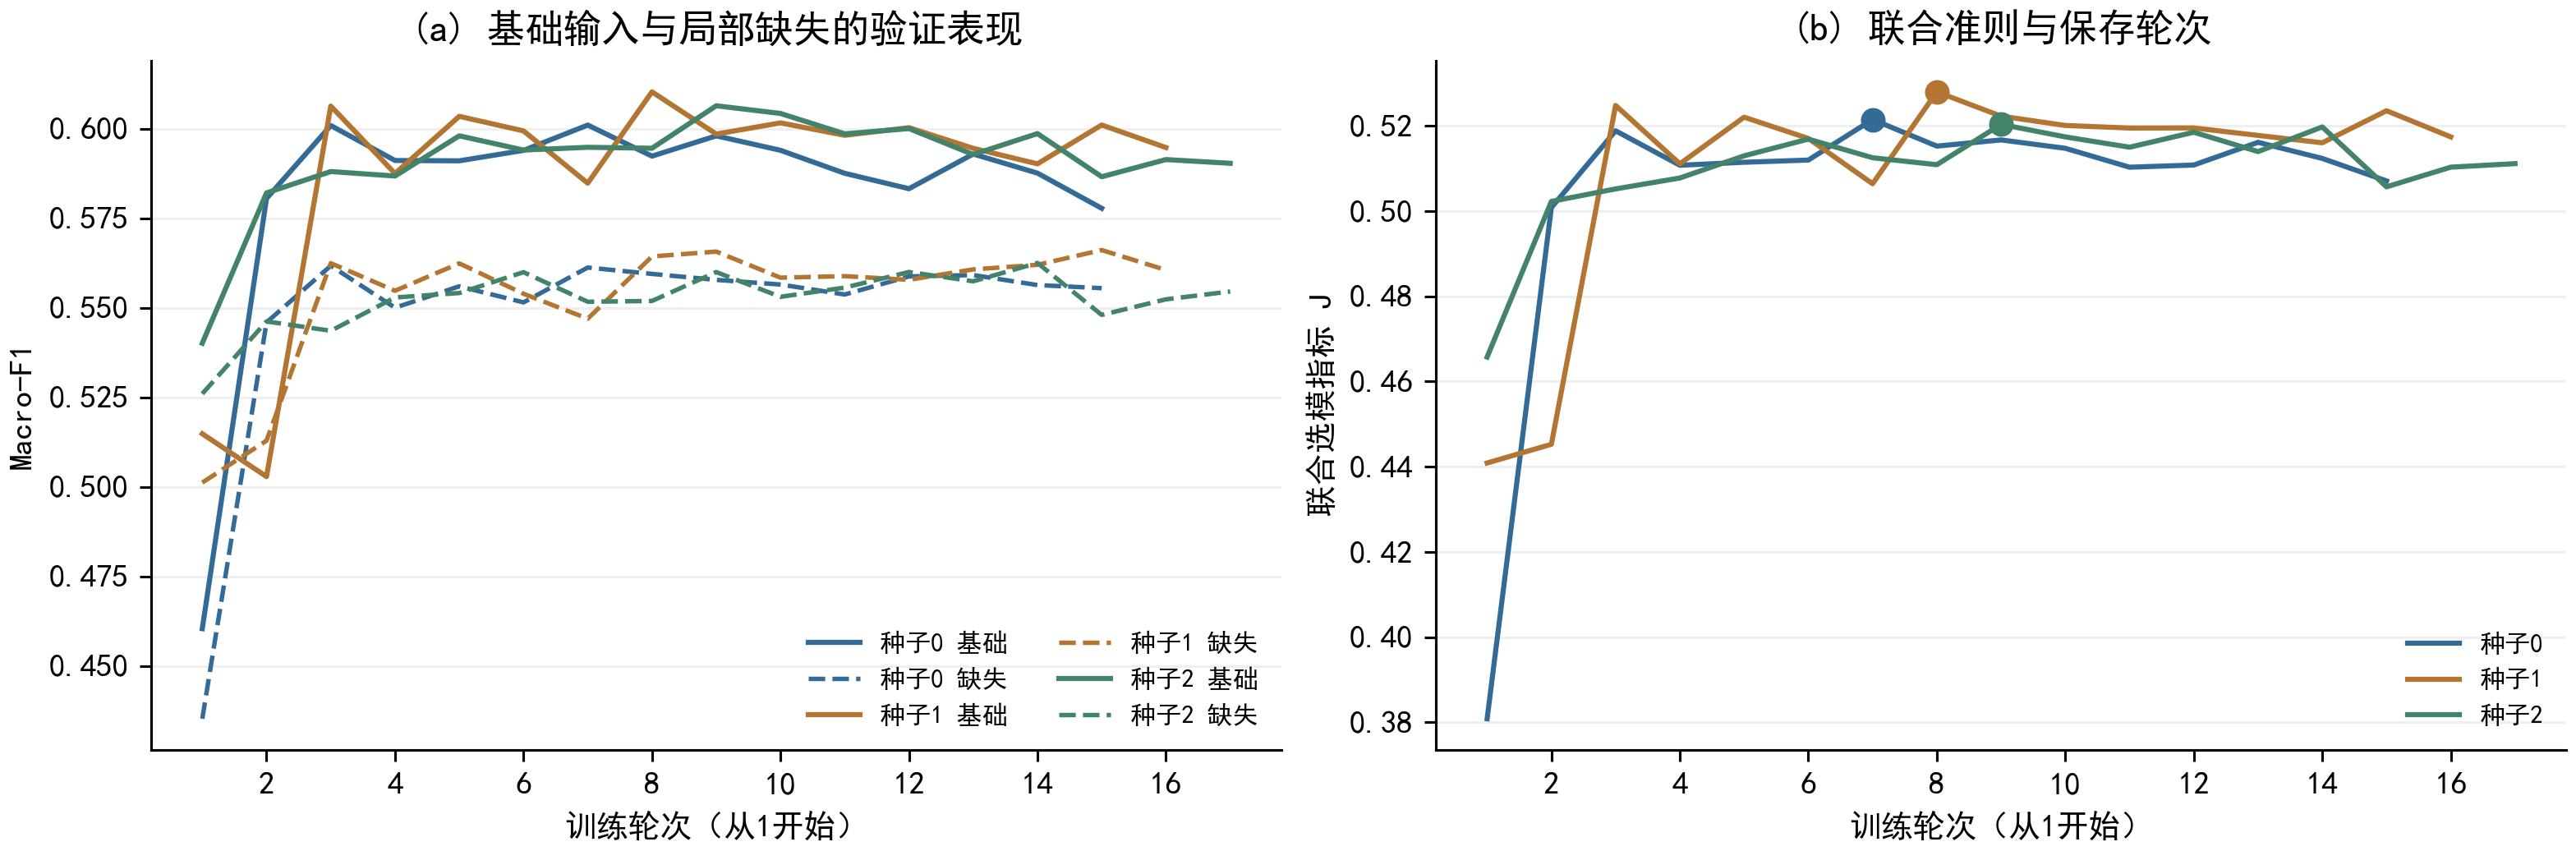
\includegraphics[width=\linewidth]{figures/q2_new_training.png}
\caption{三个学生种子的训练过程。轮次从1开始；左图实线为基础输入验证F1，虚线为四类固定局部缺口平均F1；右图为联合选模指标，圆点标记实际保存轮次。}\label{q2:fig:training}
\end{figure}
如图\ref{q2:fig:training}所示，三个种子的分类指标在训练初期较快上升，随后进入波动区间。局部缺失条件下的F1整体低于基础输入，反映出信息遮挡带来的预测损失。联合准则在基础性能与缺失性能之间进行权衡，保存其最大值对应的学生参数。

\subsubsection{实验结果与分析}
\paragraph{评价指标与基础性能}
分类采用Accuracy和Macro-F1，回归采用MAE和Pearson相关系数。Macro-F1对三类等权平均，以反映各类别的综合识别能力。评价时先对各随机种子的分类概率和强度预测取均值，再计算集成模型的指标。对照模型包括文本单模态、拼接MLP及不同缺失处理策略，种子数列于表\ref{q2:tab:base}；简单基线按基础F1选模，教师与学生按联合准则$J$选模。
\begin{table}[htbp]\centering\small
\setlength{\tabcolsep}{4pt}
\caption{基础输入下各模型性能（各自种子概率与强度集成；验证728条，测试727条）}\label{q2:tab:base}
\begin{tabularx}{\linewidth}{l*{7}{>{\centering\arraybackslash}X}}
\toprule
模型 & 种子 & \shortstack{验证\\F1} & \shortstack{验证\\MAE} & \shortstack{测试\\F1} & \shortstack{测试\\Acc} & \shortstack{测试\\MAE} & \shortstack{测试\\Pearson} \\
\midrule
仅文本 & 2 & 0.6192 & 0.6032 & 0.6077 & 0.6286 & 0.6394 & 0.6585 \\
拼接MLP & 2 & 0.6037 & 0.5926 & 0.5882 & 0.6135 & 0.6456 & 0.6512 \\
零填充 & 2 & 0.6001 & 0.5989 & 0.5877 & 0.6231 & 0.6428 & 0.6678 \\
均值填充 & 2 & 0.6044 & 0.6063 & 0.5978 & 0.6272 & 0.6490 & 0.6647 \\
缺失标记 & 2 & 0.6147 & 0.5981 & 0.5863 & 0.6176 & 0.6429 & 0.6685 \\
模态丢弃 & 2 & 0.6089 & 0.6086 & 0.5902 & 0.6272 & 0.6380 & 0.6752 \\
三态嵌入 & 3 & 0.5972 & 0.6076 & 0.6112 & 0.6437 & 0.6524 & 0.6653 \\
TSRF-D & 3 & 0.6012 & 0.5915 & 0.6138 & 0.6396 & 0.6275 & 0.6770 \\
教师 & 3 & 0.6158 & 0.5933 & 0.6053 & 0.6300 & 0.6291 & 0.6769 \\
\bottomrule
\end{tabularx}
\end{table}
表\ref{q2:tab:base}给出基础输入下各模型的双任务指标。TSRF-D在验证集上的Accuracy、Macro-F1、MAE与Pearson分别为0.6099、0.6012、0.5915与0.6448，在测试集上分别为0.6396、0.6138、0.6275与0.6770；相对文本单模态，其测试集F1高出0.0061，两个划分的MAE分别降低0.0117与0.0119。分类指标在两类输入下处于同一区间，而强度回归误差在两个划分上同时降低，三模态输入对连续强度的估计给出了一致改善。

样本级配对bootstrap检验显示，TSRF-D相对缺失标记模型的测试集F1优势为$+0.0275$（$p=0.033$）。基础输入下各模型总体处于同一性能区间，模型之间的差异更多来自局部缺失条件下的表现，下面按缺失形态分别考察。

\paragraph{局部缺失模态的影响}
在附件2测试集上固定模型权重，对不同模态组合施加长度为1、4和8的连续锚点缺口。各条件均保留自然缺失，报告实际新增遮挡占比
\begin{equation}
\eta_H=\frac{\sum_{i,m,k}H^m_{ik}}{3\sum_{i,k}P_{ik}},\qquad
\Delta F=F_H-F_{\mathrm{base}},\quad
\Delta E=\operatorname{MAE}_H-\operatorname{MAE}_{\mathrm{base}}.
\end{equation}
$\eta_H$表示人工新增缺失占全部三模态内容位置的比例，总缺失率由新增缺失与自然缺失共同构成。各模态组合按同一随机数流依次采样缺口位置，比较条件保持相同的目标长度与测试样本。
例如，长度8表示在内容序列中选取连续8个位置，将指定模态在这些位置上的观测遮挡；它度量对齐序列的跨度，单位为锚点。附件3的观测缺口长度为1至4个锚点，长度8用于检验较长中断下的性能。短于目标长度的样本按实际内容长度遮挡，此时可能覆盖该模态的全部内容位置。
\begin{table}[htbp]\centering\small
\setlength{\tabcolsep}{4pt}
\caption{局部连续缺失的模态组合结果（测试727条，三种子集成；长度单位为锚点）}\label{q2:tab:local}
\begin{tabular}{lrrrrr}
\toprule
长度 & 遮挡模态 & $\eta_H$ & Macro-F1 & MAE & $\Delta F$ \\
\midrule
1 & 文本 & 0.0144 & 0.5929 & 0.6487 & -0.0209 \\
1 & 语音 & 0.0144 & 0.6122 & 0.6271 & -0.0016 \\
1 & 视觉 & 0.0134 & 0.6137 & 0.6266 & -0.0001 \\
1 & 文本+语音 & 0.0288 & 0.6068 & 0.6477 & -0.0070 \\
1 & 文本+视觉 & 0.0276 & 0.5969 & 0.6466 & -0.0169 \\
1 & 语音+视觉 & 0.0278 & 0.6114 & 0.6269 & -0.0023 \\
1 & 文本+语音+视觉 & 0.0420 & 0.6140 & 0.6414 & +0.0002 \\
4 & 文本 & 0.0574 & 0.5581 & 0.6912 & -0.0556 \\
4 & 语音 & 0.0574 & 0.6188 & 0.6259 & +0.0050 \\
4 & 视觉 & 0.0533 & 0.6050 & 0.6254 & -0.0087 \\
4 & 文本+语音 & 0.1149 & 0.5700 & 0.6790 & -0.0438 \\
4 & 文本+视觉 & 0.1108 & 0.6025 & 0.6839 & -0.0113 \\
4 & 语音+视觉 & 0.1105 & 0.6194 & 0.6228 & +0.0056 \\
4 & 文本+语音+视觉 & 0.1685 & 0.5806 & 0.6841 & -0.0332 \\
8 & 文本 & 0.1130 & 0.5198 & 0.7334 & -0.0940 \\
8 & 语音 & 0.1130 & 0.6157 & 0.6250 & +0.0020 \\
8 & 视觉 & 0.1046 & 0.6100 & 0.6206 & -0.0038 \\
8 & 文本+语音 & 0.2260 & 0.5370 & 0.7304 & -0.0768 \\
8 & 文本+视觉 & 0.2177 & 0.5311 & 0.7357 & -0.0827 \\
8 & 语音+视觉 & 0.2179 & 0.6227 & 0.6209 & +0.0090 \\
8 & 文本+语音+视觉 & 0.3309 & 0.5332 & 0.7406 & -0.0806 \\
\bottomrule
\end{tabular}
\end{table}
\begin{figure}[htbp]\centering
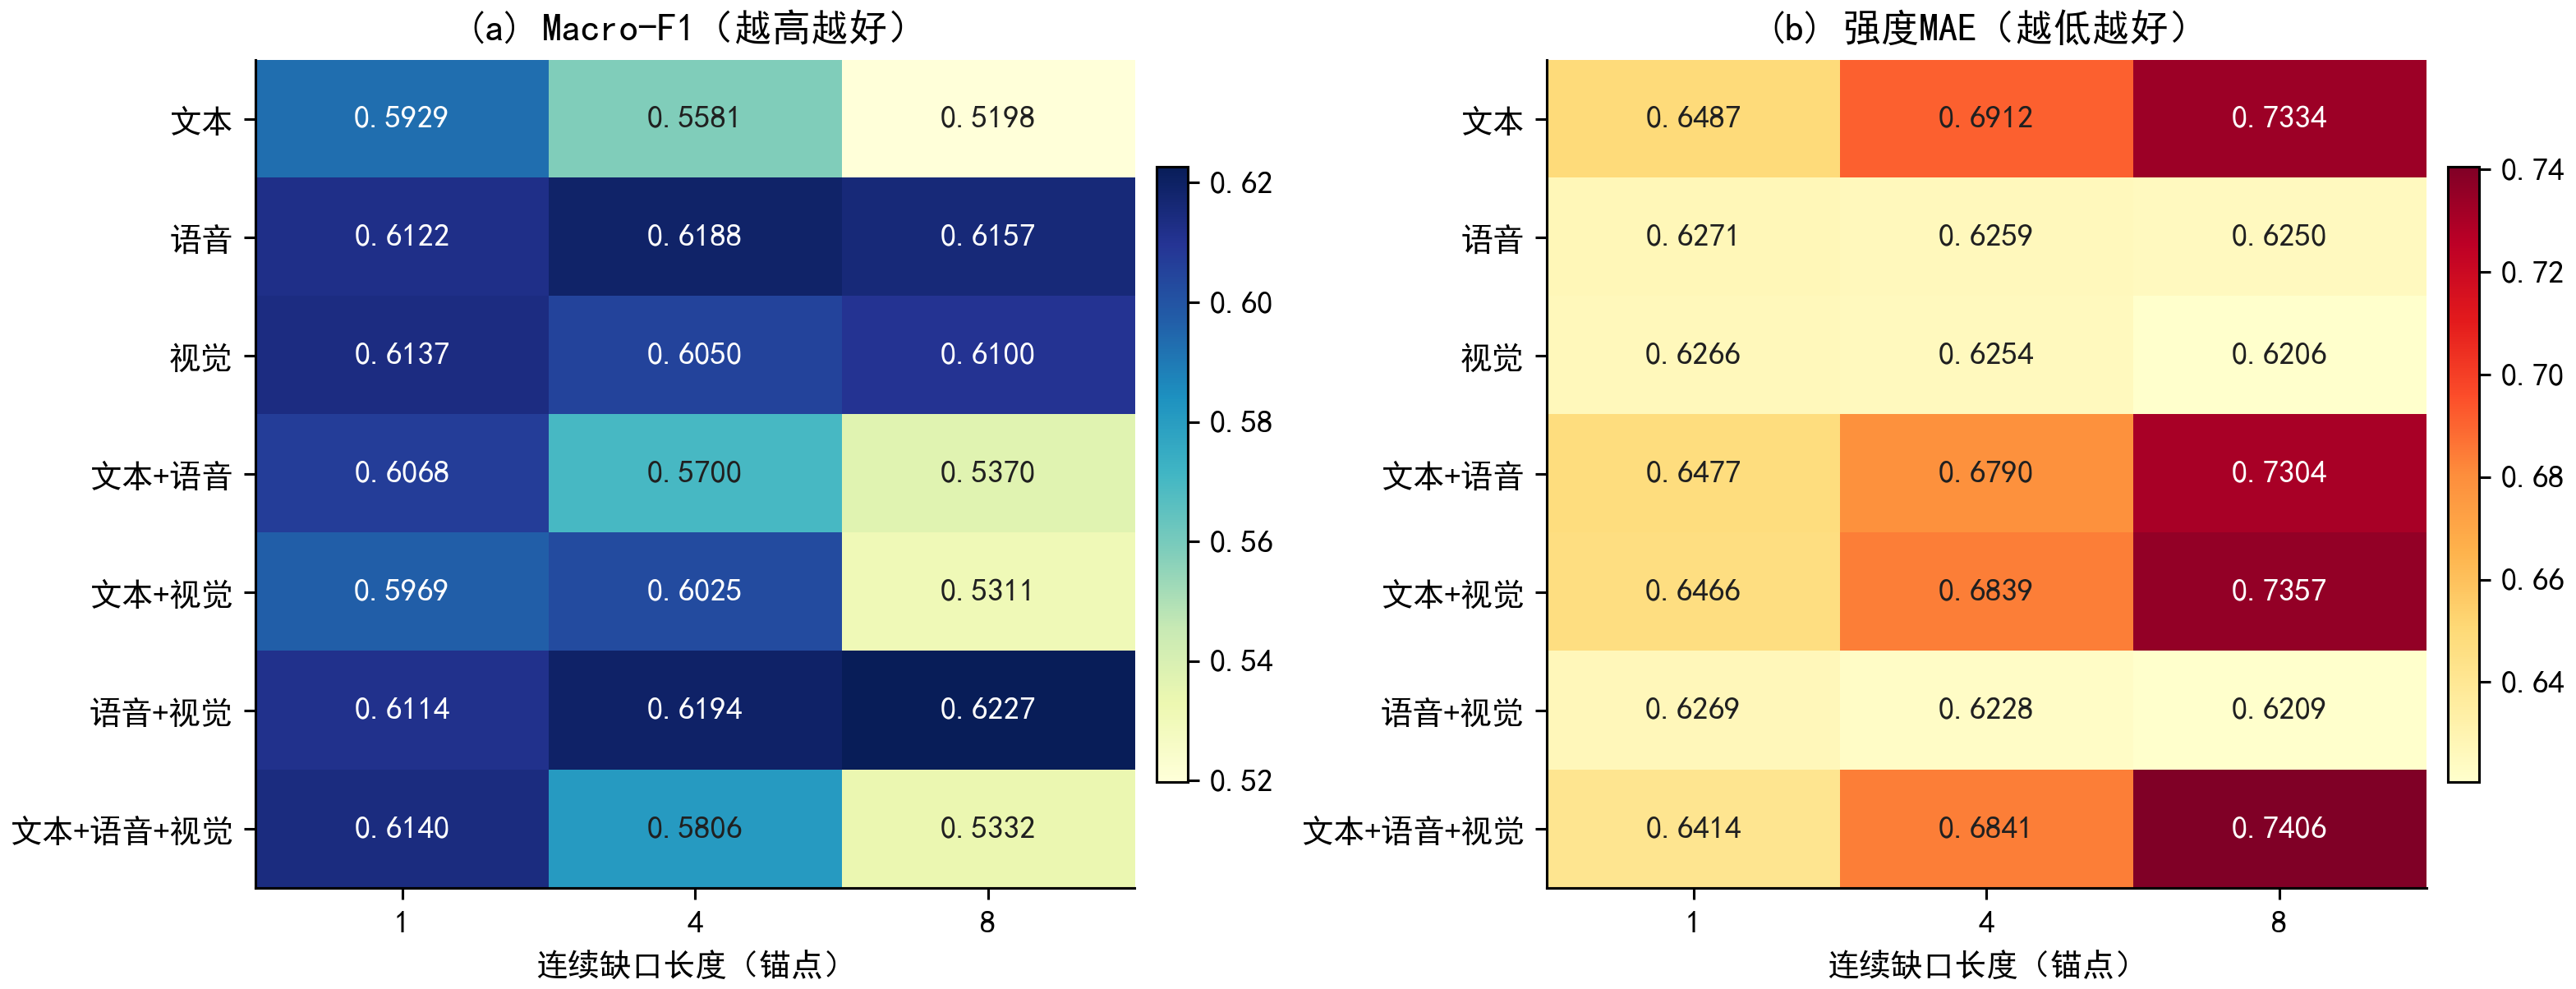
\includegraphics[width=\linewidth]{figures/q2_new_local.png}
\caption{不同模态组合与连续缺口长度下的预测性能。左：Macro-F1；右：强度MAE。}\label{q2:fig:local}
\end{figure}
表\ref{q2:tab:local}与图\ref{q2:fig:local}表明，涉及文本的缺失组合对缺口长度最为敏感：8锚点缺口下，仅文本缺失使F1由0.6138降至0.5198、MAE由0.6275升至0.7334，且退化幅度随长度由1增至8逐档放大；仅语音、仅视觉缺失时F1分别为0.6157与0.6100，与基础输入接近；三模态同段缺失时F1为0.5332、MAE为0.7406。文本承担了较多的情感判别信息，文本缺口是局部缺失条件下的主要困难；音视频通道在文本完整时的边际贡献相对有限，却在文本失效时提供补偿。

\paragraph{缺失位置、长度与比例的影响}
设置三组敏感性实验：位置实验分别遮挡内容首段、中段和尾段约三分之一的连续位置；长度实验随机放置1、2、4、8、16锚点的三模态共缺区间，短样本按有效长度截断，其实际新增遮挡量$\eta_H$由4.20\%增至60.71\%，构成连续区间口径下的缺失率序列；比例实验采用随机点状遮挡，在各模态观测位置中按指定比例抽样，构成分散缺失口径下的缺失率序列。前两组分析连续区间缺失，第三组分析分散缺失带来的影响。
\begin{table}[htbp]\centering\small
\setlength{\tabcolsep}{4pt}
\caption{位置、连续缺口长度与随机点状比例实验（测试727条，三种子集成）；前两项分析连续区间缺失，第三项分析分散缺失}\label{q2:tab:factors}
\begin{tabular}{lrrrrr}
\toprule
条件 & $\eta_H$ & Macro-F1 & MAE & $\Delta F$ & $\Delta\mathrm{MAE}$ \\
\midrule
位置：句首 & 0.3278 & 0.5638 & 0.6816 & -0.0499 & +0.0541 \\
位置：句中 & 0.3276 & 0.5738 & 0.7011 & -0.0400 & +0.0736 \\
位置：句尾 & 0.3257 & 0.5747 & 0.6904 & -0.0391 & +0.0629 \\
长度：1 & 0.0420 & 0.5906 & 0.6438 & -0.0232 & +0.0163 \\
长度：2 & 0.0842 & 0.5967 & 0.6619 & -0.0171 & +0.0344 \\
长度：4 & 0.1680 & 0.5739 & 0.6967 & -0.0399 & +0.0692 \\
长度：8 & 0.3307 & 0.5410 & 0.7412 & -0.0728 & +0.1136 \\
长度：16 & 0.6071 & 0.4462 & 0.8026 & -0.1676 & +0.1751 \\
点状比例：0.05 & 0.0479 & 0.6074 & 0.6352 & -0.0064 & +0.0077 \\
点状比例：0.10 & 0.0984 & 0.5822 & 0.6662 & -0.0316 & +0.0387 \\
点状比例：0.20 & 0.1975 & 0.5832 & 0.6761 & -0.0306 & +0.0486 \\
点状比例：0.30 & 0.2929 & 0.5711 & 0.7141 & -0.0427 & +0.0865 \\
点状比例：0.40 & 0.3917 & 0.5469 & 0.7316 & -0.0668 & +0.1041 \\
\bottomrule
\end{tabular}
\end{table}
\begin{figure}[htbp]\centering
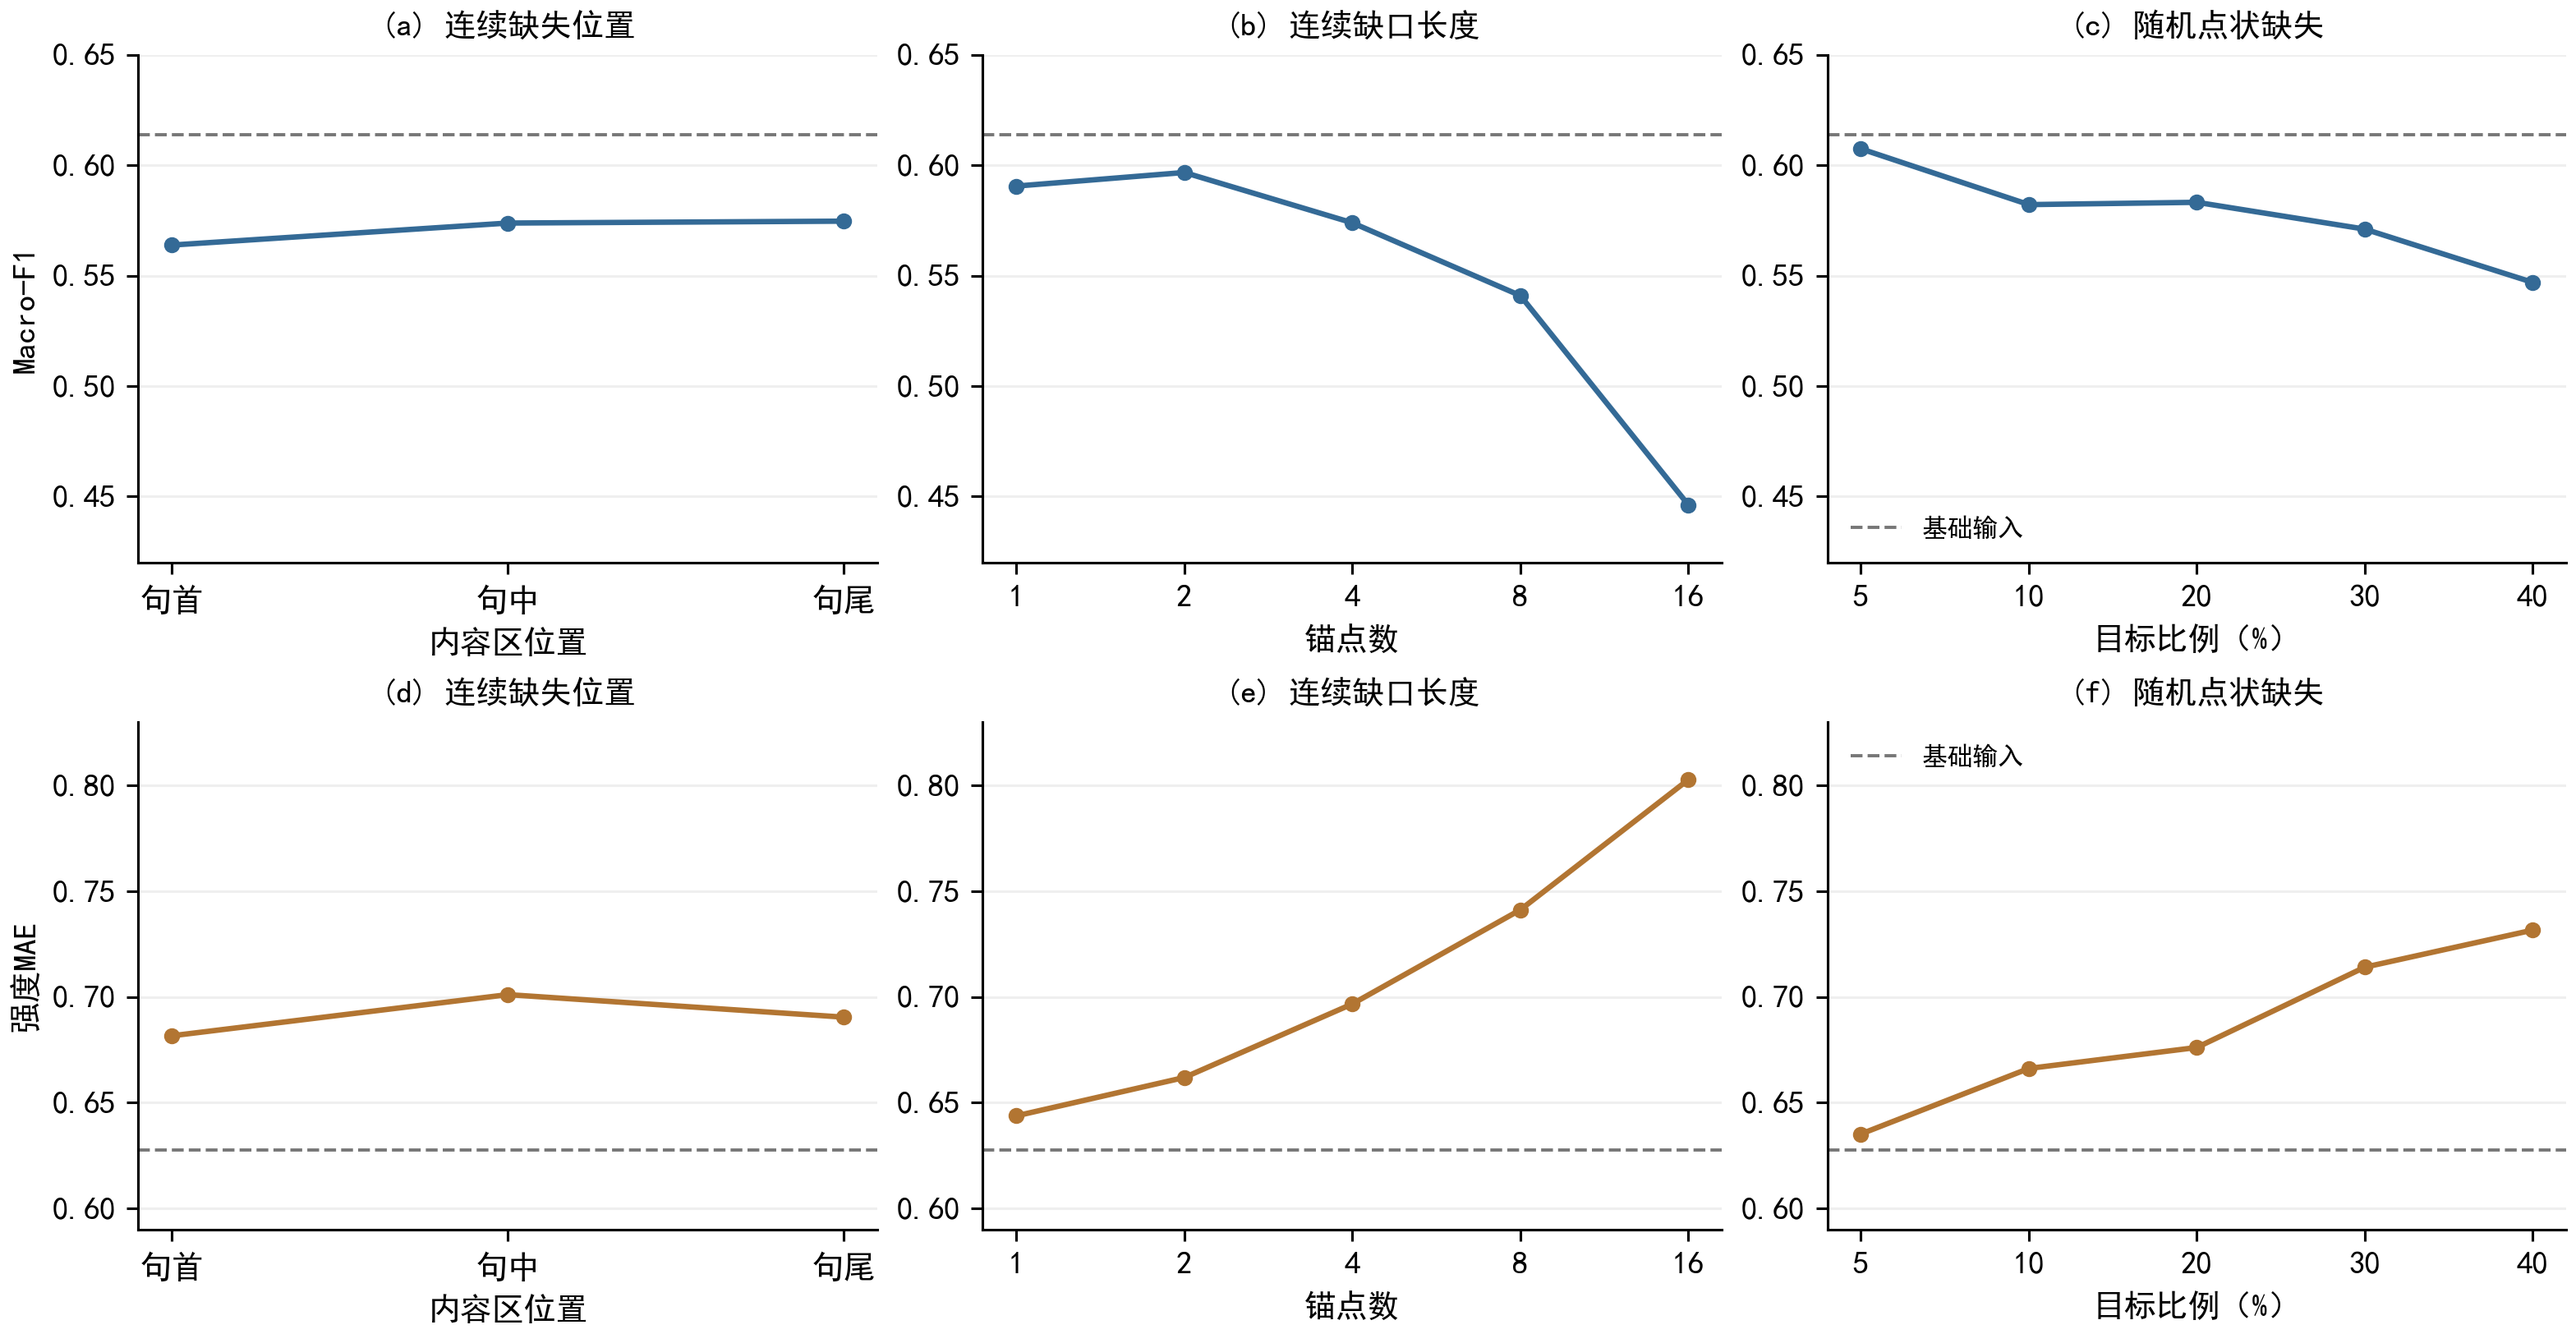
\includegraphics[width=\linewidth]{figures/q2_new_factors.png}
\caption{缺失位置、连续缺口长度与随机点状缺失比例的敏感性。上排为Macro-F1，下排为MAE；灰色虚线表示基础输入性能。横轴比例为目标抽样比例，实际新增遮挡占比见表\ref{q2:tab:factors}。}\label{q2:fig:factors}
\end{figure}
由表\ref{q2:tab:factors}和图\ref{q2:fig:factors}可知，句首遮挡对应最低F1（0.5638），句中遮挡对应最高MAE（0.7011）。三种位置的F1极差为0.0108，位置效应小于模态类型与缺口长度的影响。缺口长度由1增加至16个锚点时，F1总体由0.5906降至0.4462，MAE由0.6438升至0.8026；其中长度2的F1略高于长度1，表明分类变化并非逐档单调。长度16同时对应60.71\%的实际新增遮挡量，故该结果体现连续跨度与信息损失数量的共同影响。

随机点状缺失比例从5\%增加至40\%时，F1从0.6074降至0.5469，MAE从0.6352升至0.7316。两项指标整体随缺失程度增加而退化，其中F1在个别相邻比例间出现小幅波动。连续缺口实验与随机点状实验共同反映了缺失几何和缺失数量对预测的影响。

两组序列的实际新增遮挡量区间相近，可在同一缺失程度坐标下比较缺失几何的影响。图\ref{q2:fig:ratecurve}给出相应曲线：在实际新增遮挡量约4\%--5\%处，连续缺口与随机点状的F1分别为0.5906与0.6074；在约33\%处，连续缺口的F1为0.5410，低于随机点状在29.29\%与39.17\%处的0.5711与0.5469，强度MAE呈现同向差异（0.7412对0.7141与0.7316）。在相近甚至更高的缺失数量下，随机点状缺失的性能仍高于连续缺口，说明除信息损失数量外，缺失在时间上的聚集方式同样影响预测。长度实验对短样本按有效长度整段截断，该序列同时包含整段覆盖带来的影响。

\begin{figure}[htbp]\centering
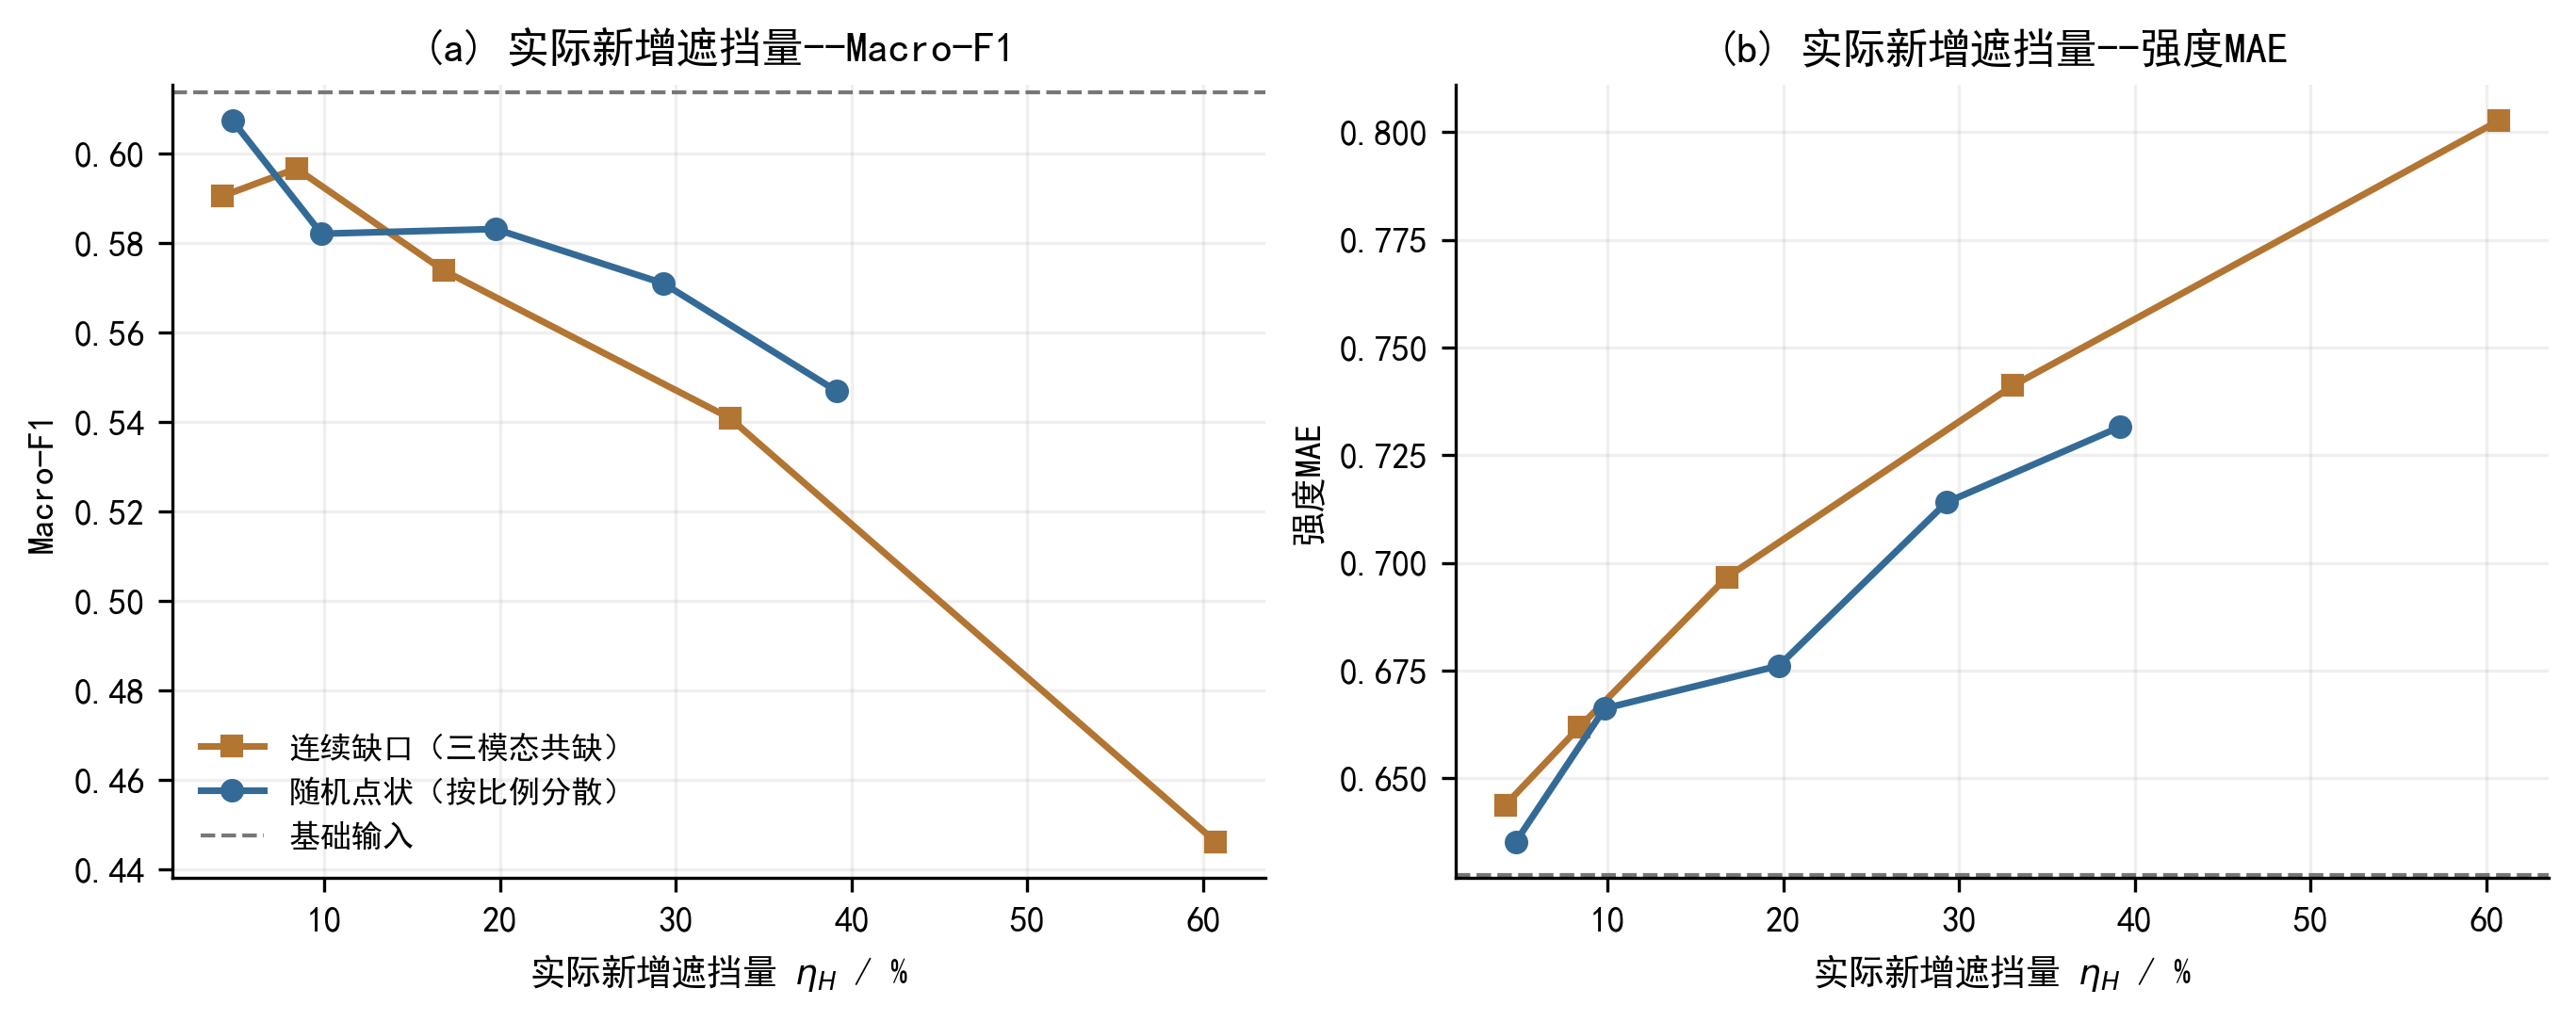
\includegraphics[width=\linewidth]{figures/q2_rate_curve.png}
\caption{实际新增遮挡量$\eta_H$与预测性能的关系。左：Macro-F1；右：强度MAE。连续缺口为长度1--16锚点的三模态共缺区间，随机点状为按比例分散遮挡；灰色虚线为基础输入性能。}\label{q2:fig:ratecurve}
\end{figure}
需要说明三组实验的口径差异：模态组合实验与长度实验各自采样缺口位置，同为长度8的三模态共缺，两处分别得到0.5332与0.5410，差别来自遮挡位置不同；位置实验则保持同一样本的目标长度不变，仅把区间移动到句首、句中与句尾，实际新增遮挡量的细微差别只源于自然缺失的分布。

整模态删除给出信息减少到极限时的参照：文本整体缺失时F1为0.4088，三模态全缺时为0.1190。前者仍保留音视频观测，模型借此完成跨模态补偿，F1保持在0.40以上；后者补全候选集为空、触发回退，性能降至0.12附近。两者的差值刻画了跨模态补偿在极端条件下的作用幅度。

\paragraph{缺失条件下的消融与补全机制验证}
为检验蒸馏、补全与可靠度监督各自的作用，在相同测试样本、相同固定干预掩码下比较关闭或替换相应模块后的预测性能，以排除掩码差异带来的干扰。各配置均使用三个种子，并采用与主模型一致的概率集成口径。结果列于表\ref{q2:tab:ablstress}：基础输入列给出各配置在无新增缺失时的性能，用于区分模块自身的影响与缺失条件下的影响；连续段缺口列为句首、句中、句尾三种连续区间的Macro-F1均值，与表\ref{q2:tab:factors}的位置实验共用同一组掩码，对应实际新增遮挡量约32.6\%。

\begin{table}[htbp]\centering\small
\setlength{\tabcolsep}{4pt}
\caption{补充压力条件下的消融Macro-F1（测试727条，各配置三种子概率集成；连续段缺口为句首、句中、句尾三种连续区间的均值）}\label{q2:tab:ablstress}
\begin{tabular}{lrrrrr}
\toprule
配置 & 基础输入 & 连续段缺口 & 点状20\% & 点状40\% & 整缺文本 \\
\midrule
TSRF-D & 0.6138 & 0.5708 & 0.5716 & 0.5490 & 0.4088 \\
关闭全部蒸馏 & 0.6034 & 0.5763 & 0.5820 & 0.5467 & 0.4186 \\
仅分类蒸馏 & 0.6096 & 0.5736 & 0.5670 & 0.5472 & 0.4166 \\
仅强度蒸馏 & 0.6082 & 0.5802 & 0.5769 & 0.5449 & 0.4169 \\
关闭补全分支 & 0.6087 & 0.5725 & 0.5907 & 0.5421 & 0.4155 \\
关闭可靠度监督 & 0.6068 & 0.5783 & 0.5667 & 0.5507 & 0.4048 \\
仅同模态候选 & 0.6122 & 0.5717 & 0.5618 & 0.5396 & 0.3815 \\
仅跨模态候选 & 0.6132 & 0.5788 & 0.5788 & 0.5595 & 0.4014 \\
关闭观测连续性项 & 0.6054 & 0.5730 & 0.5649 & 0.5544 & 0.4022 \\
置信度加权蒸馏 & 0.6052 & 0.5755 & 0.5800 & 0.5400 & 0.4452 \\
\bottomrule
\end{tabular}
\end{table}
按组件逐项看：蒸馏的作用与缺失强度相关，随机20\%缺失时关闭全部蒸馏使F1由0.5716升至0.5820，而在随机40\%缺失时由0.5490降至0.5467；补全分支呈现同一方向，两种条件下分别变化$+0.0191$与$-0.0069$，说明其收益随缺失强度而变。候选来源方面，40\%缺失下仅跨模态候选的F1为0.5595，高于仅同模态候选的0.5396，高缺失程度下跨模态信息的补偿作用更为明显。在相同连续区间条件下，各配置的F1介于0.5708与0.5802之间，极差0.0094，小于点状缺失下的配置差异，说明共享连续缺口时组件之间的差异收敛。需要说明两组消融的口径：消融组内部共用固定掩码，但与敏感性实验采用各自独立的遮挡实现，故两表中20\%与40\%条件的数值分别对应其掩码；连续段缺口列与位置实验使用同一组掩码，用于在共享连续区间内比较组件作用。

为分析补全质量，在验证集设置四类居中8锚点缺口，以遮挡前的标准化特征为真值，比较学习补全、模型回退和均值填充的MAE。三个种子与四类条件共形成50388条位置记录，结果按模态汇总于表\ref{q2:tab:recon}。记录数包含样本在不同条件和种子下的重复评价。
\begin{table}[htbp]\centering\small
\setlength{\tabcolsep}{4pt}
\caption{人工遮挡位的特征重建MAE（验证集；记录数含多种子及多条件重复）}\label{q2:tab:recon}
\begin{tabular}{lrrrrr}
\toprule
模态 & 记录数 & 补全 & 回退 & 均值填充 & 回退减补全 \\
\midrule
总体 & 50388 & 0.7140 & 0.7401 & 0.7407 & +0.0260 \\
文本 & 17142 & 0.7817 & 0.7852 & 0.7841 & +0.0035 \\
语音 & 17118 & 0.6618 & 0.6794 & 0.6787 & +0.0176 \\
视觉 & 16128 & 0.6975 & 0.7564 & 0.7605 & +0.0589 \\
\bottomrule
\end{tabular}
\end{table}
\begin{figure}[htbp]\centering
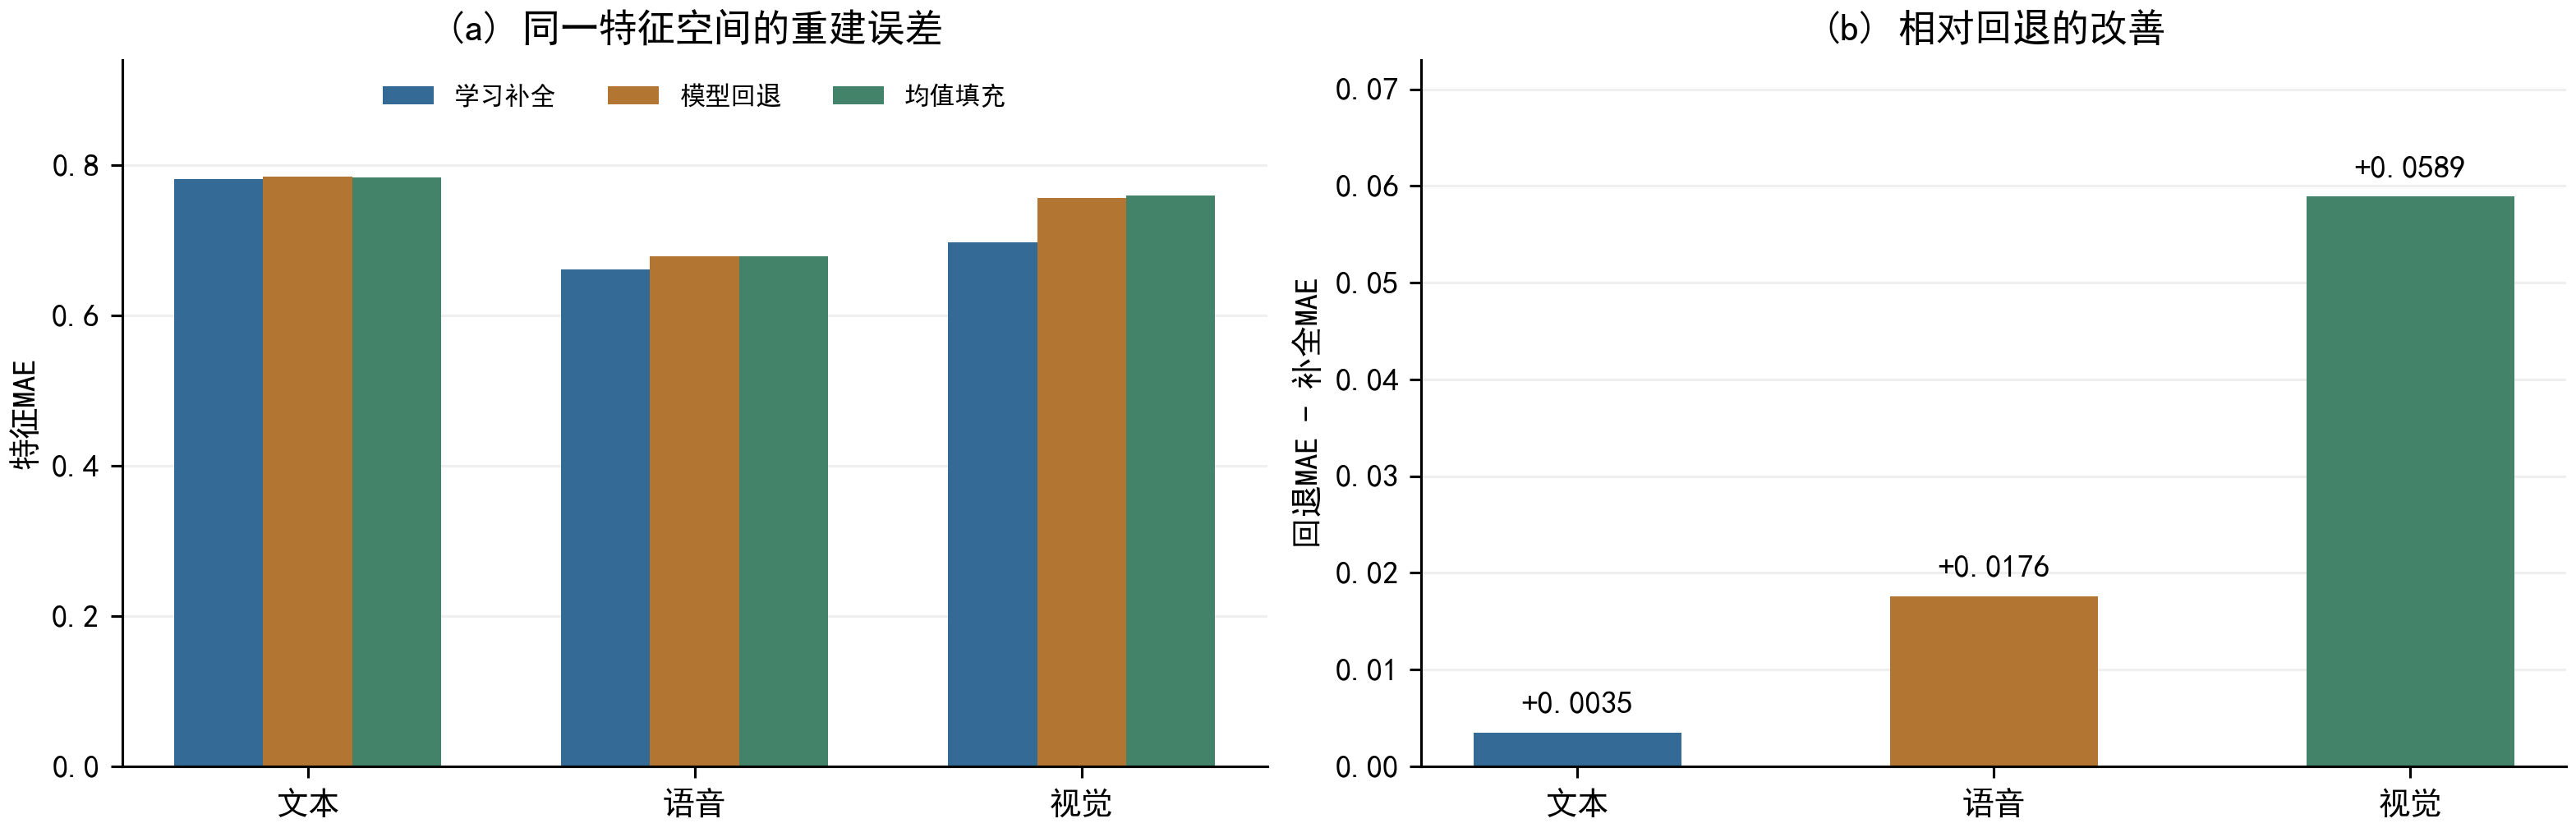
\includegraphics[width=\linewidth]{figures/q2_new_reconstruction.png}
\caption{逐模态补全效果。左：补全、回退及均值填充的特征MAE；右：相对回退的MAE下降量。}\label{q2:fig:recon}
\end{figure}
图\ref{q2:fig:recon}给出逐模态的补全效果：学习补全相对回退使总体MAE下降0.0260，约78.8\%的位置记录获得改善；分模态看，视觉、语音与文本的MAE分别下降0.0589、0.0176与0.0035。视觉特征在标准化空间中的可重建性最好，而文本遮挡造成的预测退化最大，二者共同说明特征空间的近似误差与语义信息的丢失并不同质：数值上可重建的模态未必对预测最关键，文本缺口因而是后续优化的重点。

可靠度是否可用，取决于它与重建误差的实际关系：总体Pearson相关系数为$-0.0625$，以“误差低于中位数”为正类的AUC为0.6664；分模态计算时AUC为0.5120、0.4392与0.5575，均低于混合统计，说明该判别力来自跨模态位置的误差尺度差异，而非单一模态内部的误差排序。上述指标在重复位置记录上评价绝对重建误差，与训练中相对回退的监督目标互为补充，分别刻画“特征是否被重建”与“重建是否优于回退”。门控取值干预直接检验融合权重的作用：固定$\rho\equiv0$时平均F1比学习门控低0.0133，说明补全表示确实携带任务信息；固定$\rho\equiv1$与学习门控的平均F1相差0.0039，两者处于同一水平。

\paragraph{验证集可视化与错误归因}
\begin{figure}[htbp]\centering
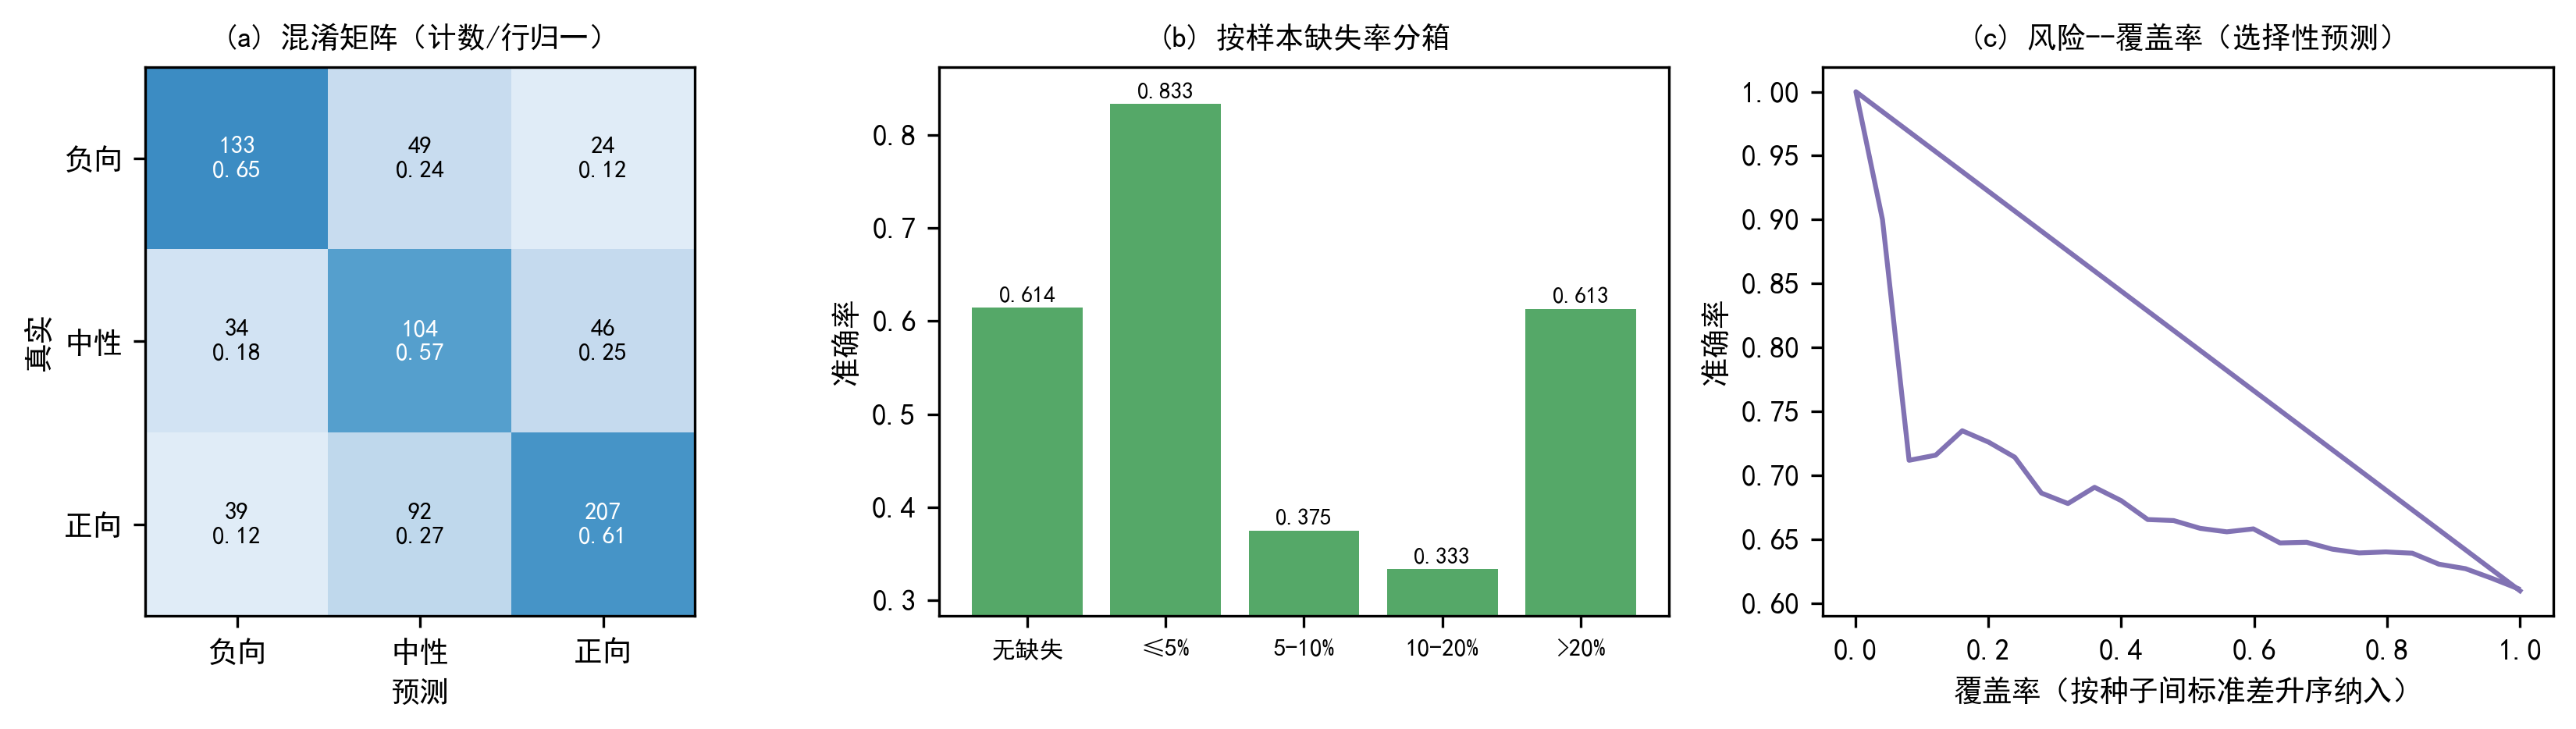
\includegraphics[width=\linewidth]{figures/q2_fig6_valid_confusion.png}
\caption{验证集分类混淆矩阵、自然缺失分组准确率与覆盖率分析。}\label{q2:fig:valid}
\end{figure}
验证集三类F1分别为负向0.6456、中性0.4848、正向0.6732。混淆矩阵中，206条负向样本有49条判为中性；338条正向样本有92条判为中性；184条中性样本中有34条判为负向、46条判为正向。共284条误判中，221条涉及中性类，约占77.8\%，表明中性与正、负情感之间的混淆是主要错误类型。

中性类精确率为0.4245，极性样本与中性样本的交界区间构成分类判别的主要着力点。结合文本缺失实验，文本证据的保留与中性边界的刻画是提高预测性能的两个重点；受控遮挡实验给出不同缺失条件下的性能变化。

\FloatBarrier
\paragraph{附件3全量预测与结果展示}
冻结三个学生模型，分别输出分类概率和连续强度，再取算术平均：
\begin{equation}
\bar p_i=\frac13\sum_{s=0}^{2}p_i^{(s)},\qquad
\hat y_i=\arg\max_c\bar p_{ic},\qquad
\bar r_i=\frac13\sum_{s=0}^{2}\hat r_i^{(s)}.
\end{equation}
专项推理由冻结学生独立完成，以未经校准的最大类别概率$c_i=\max_c\bar p_{ic}$衡量类别分布的集中程度，并同时记录种子间的预测标准差。

附件3的30条样本均完成预测，其中负向7条、中性11条、正向12条。最大类别概率均值为0.5939，最小为0.3694，13条样本低于0.5。全部样本均满足可用锚点数量规则，未触发兜底标记。附件3为无标签专项集，本节汇总其预测分布与逐样本结果。

\begin{figure}[htbp]\centering
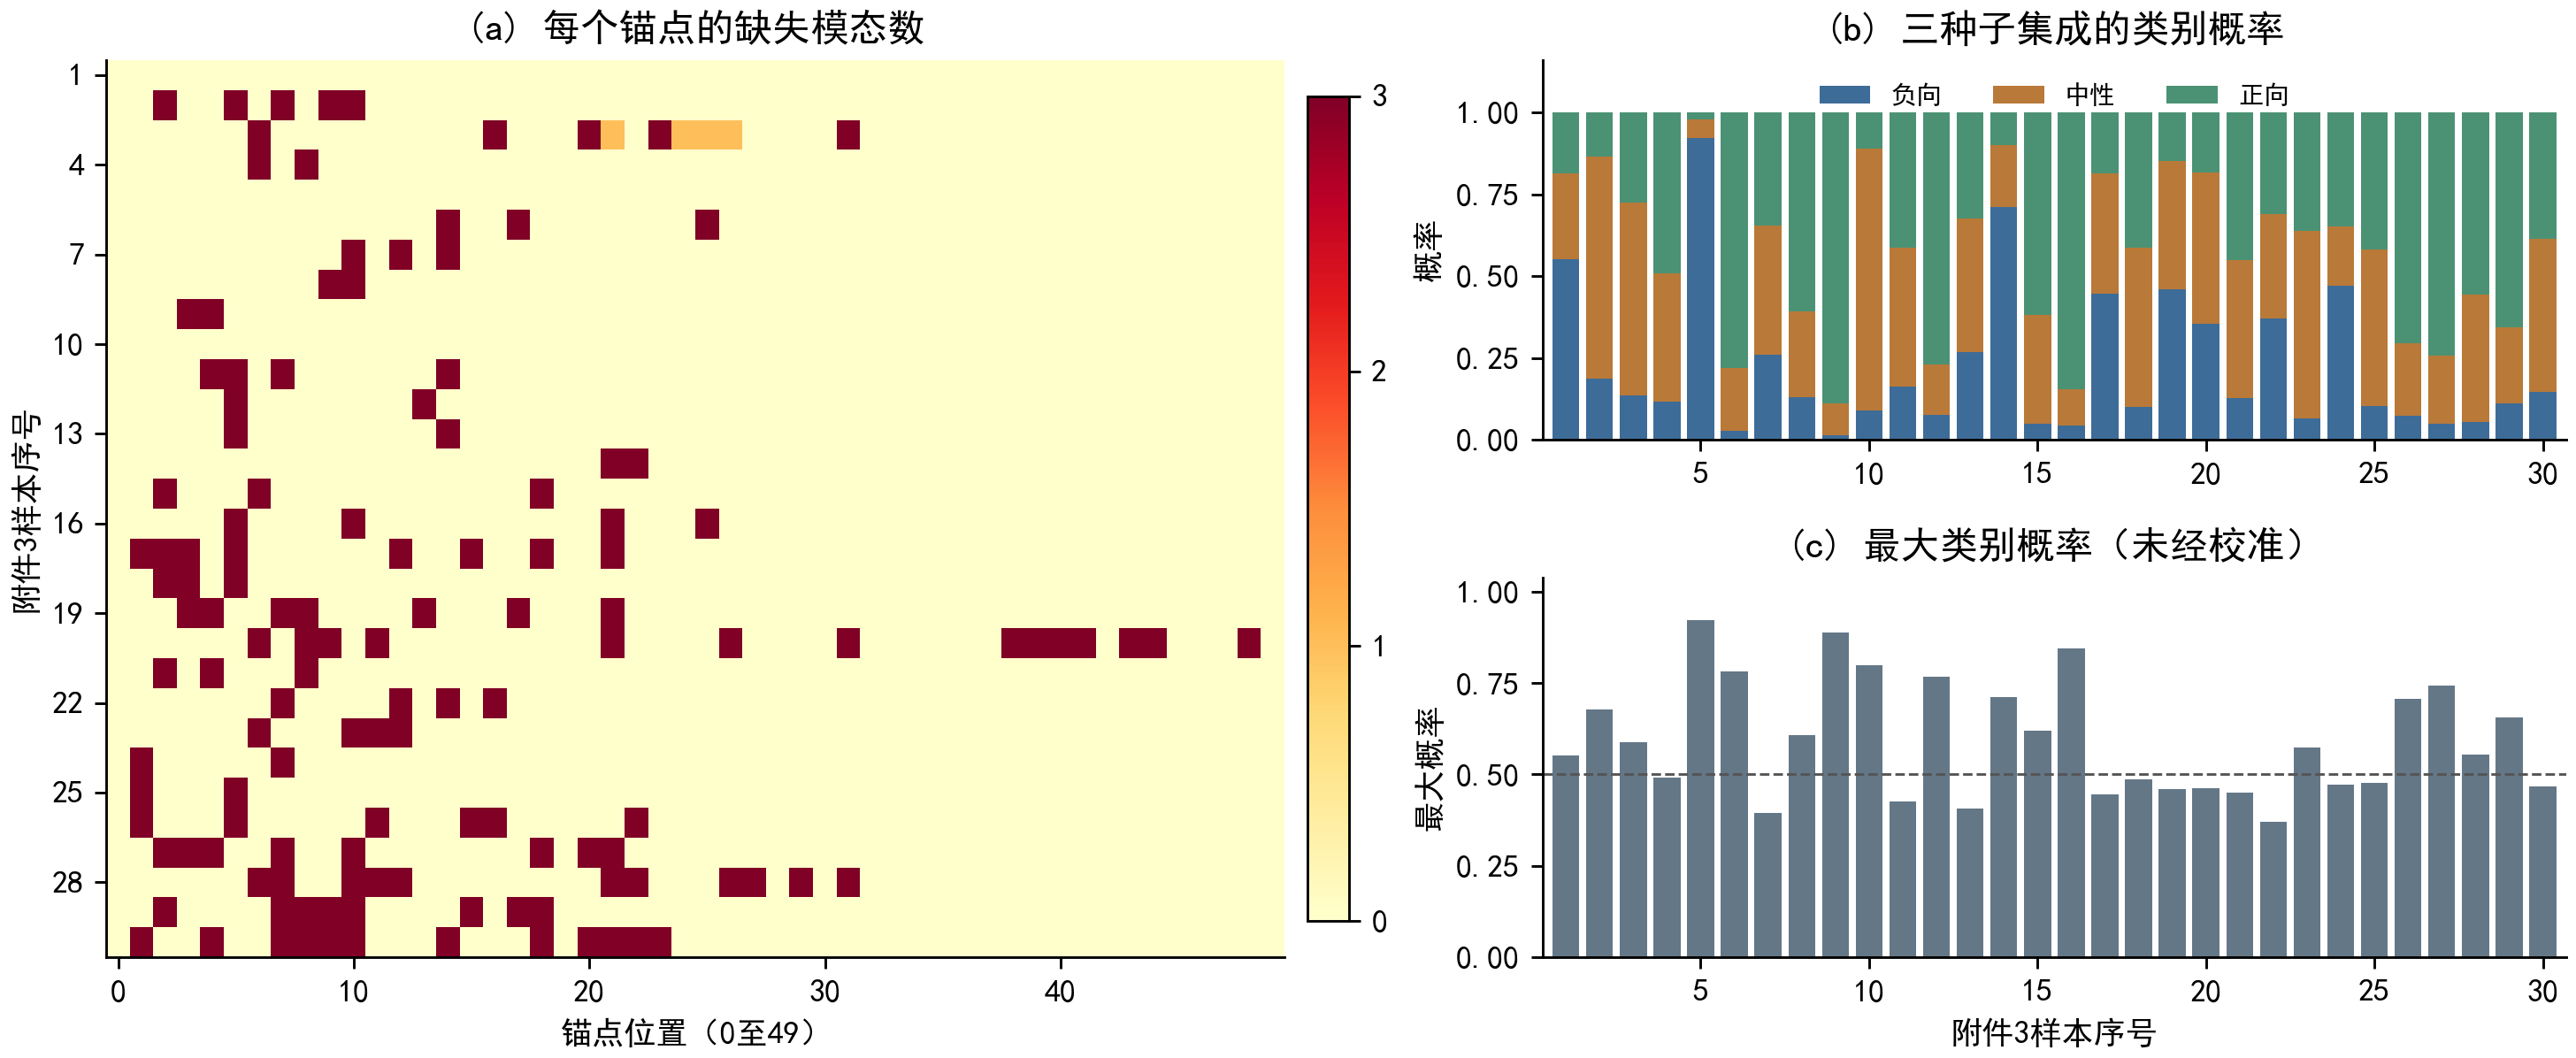
\includegraphics[width=\linewidth]{figures/q2_fig7_a3_overview.png}
\caption{附件3的缺失结构、三分类概率及最大类别概率。热力图表示缺失模态数量，0也包含结构填充位置；虚线0.5仅作概率参照，不用于拒识。}\label{q2:fig:a3}
\end{figure}

表\ref{q2:tab:a3}列出全部30条样本的编号、内容长度、模态缺失计数、缺失率、预测极性、连续强度与最大类别概率，三类概率、种子间标准差与诊断标记一并写入预测结果文件。
{\small
\setlength{\tabcolsep}{4pt}
\begin{longtable}{lrrrrrr}
\caption{附件3全部30条预测（缺失计数依次为文本/语音/视觉；最大概率未经校准）}\label{q2:tab:a3}\\
\toprule
编号 & 锚点数 & 缺失计数 & 缺失率 & 极性 & 连续强度 & 最大概率 \\
\midrule
\endfirsthead
\toprule
编号 & 锚点数 & 缺失计数 & 缺失率 & 极性 & 连续强度 & 最大概率 \\
\midrule
\endhead
\midrule
\multicolumn{7}{r}{续下页}\\
\endfoot
\bottomrule
\endlastfoot
3-01 & 6 & 0/0/0 & 0.0000 & 负向 & -0.5468 & 0.5510 \\
3-02 & 28 & 5/5/5 & 0.1786 & 中性 & -0.0340 & 0.6782 \\
3-03 & 32 & 5/5/9 & 0.1979 & 中性 & +0.2972 & 0.5889 \\
3-04 & 31 & 2/2/2 & 0.0645 & 正向 & +0.4812 & 0.4923 \\
3-05 & 12 & 0/0/0 & 0.0000 & 负向 & -1.3953 & 0.9228 \\
3-06 & 25 & 3/3/3 & 0.1200 & 正向 & +0.9457 & 0.7818 \\
3-07 & 21 & 3/3/3 & 0.1429 & 中性 & +0.2034 & 0.3952 \\
3-08 & 15 & 2/2/2 & 0.1333 & 正向 & +0.7475 & 0.6083 \\
3-09 & 14 & 2/2/2 & 0.1429 & 正向 & +1.1769 & 0.8901 \\
3-10 & 6 & 0/0/0 & 0.0000 & 中性 & +0.0221 & 0.8000 \\
3-11 & 14 & 4/4/4 & 0.2857 & 中性 & +0.3927 & 0.4260 \\
3-12 & 13 & 2/2/2 & 0.1538 & 正向 & +1.1345 & 0.7688 \\
3-13 & 19 & 2/2/2 & 0.1053 & 中性 & +0.1896 & 0.4078 \\
3-14 & 23 & 2/2/2 & 0.0870 & 负向 & -0.5930 & 0.7110 \\
3-15 & 27 & 3/3/3 & 0.1111 & 正向 & +0.6544 & 0.6194 \\
3-16 & 34 & 4/4/4 & 0.1176 & 正向 & +1.3189 & 0.8447 \\
3-17 & 22 & 8/8/8 & 0.3636 & 负向 & -0.1464 & 0.4464 \\
3-18 & 17 & 3/3/3 & 0.1765 & 中性 & +0.4361 & 0.4876 \\
3-19 & 24 & 7/7/7 & 0.2917 & 负向 & -0.2082 & 0.4608 \\
3-20 & 48 & 14/14/14 & 0.2917 & 中性 & -0.1412 & 0.4622 \\
3-21 & 9 & 3/3/3 & 0.3333 & 正向 & +0.3313 & 0.4513 \\
3-22 & 17 & 4/4/4 & 0.2353 & 负向 & +0.0996 & 0.3694 \\
3-23 & 13 & 4/4/4 & 0.3077 & 中性 & +0.3399 & 0.5748 \\
3-24 & 8 & 2/2/2 & 0.2500 & 负向 & -0.0593 & 0.4709 \\
3-25 & 9 & 2/2/2 & 0.2222 & 中性 & +0.4343 & 0.4780 \\
3-26 & 22 & 6/6/6 & 0.2727 & 正向 & +0.7859 & 0.7061 \\
3-27 & 21 & 8/8/8 & 0.3810 & 正向 & +0.7377 & 0.7438 \\
3-28 & 33 & 11/11/11 & 0.3333 & 正向 & +0.5745 & 0.5556 \\
3-29 & 18 & 8/8/8 & 0.4444 & 正向 & +0.7135 & 0.6559 \\
3-30 & 24 & 12/12/12 & 0.5000 & 中性 & +0.3798 & 0.4671 \\
\end{longtable}
}
两类样本给出缺失程度的对照：样本3-05不含人工缺失，负向概率0.9228、强度$-1.3953$，两个输出头一致给出明确的负向判断；样本3-30三模态各缺失12个锚点（缺失率50\%），仍给出中性概率0.4671与强度$+0.3798$，极性与强度同时落在中性区间，表明中等缺失程度下双任务输出仍保持一致。

样本3-22的类别输出为负向，强度为$+0.0996$，最大类别概率仅0.3694。当强度接近零点时，类别判别与强度估计表现出不同的敏感度，两个输出头因此出现方向分歧；结果表保留双头的原始预测，不做一致性修正。

专项结果按附件3的编号顺序输出，一行对应一个样本；类别编号0、1、2分别为负向、中性、正向，缺失计数以内容锚点为单位，三模态缺失率的分母为三倍内容长度。输出文件同时保留三类概率、预测集中度、种子间波动与可用锚点数。

接口一致性以附件2与附件3的重合样本核验：两条加载路径下的最大概率差约为$1.55\times10^{-6}$，最大强度差约为$4.95\times10^{-6}$，均处于浮点误差量级，表明训练数据与专项数据经过同一套加载流程。

\FloatBarrier
\paragraph{结果讨论与改进方向}
TSRF-D通过三态表示、观测节点补全与教师--学生训练，在局部信息缺失时完成极性与强度的联合预测。验证集Macro-F1为0.6012、强度MAE为0.5915，附件2测试集分别为0.6138与0.6275。受控遮挡实验说明三个因素的作用并不等价：模态类型的影响最大，8锚点文本缺口使F1由0.6138降至0.5198，而同等语音、视觉缺口下F1分别保持在0.6157与0.6100；缺口长度其次，连续缺口由1增至16个锚点时F1总体由0.5906降至0.4462；区间位置的影响最小，句首、句中、句尾三种位置的F1极差仅0.0108。

TSRF-D在文本整体缺失时借助音视频观测完成跨模态补偿，三模态同段缺失8锚点时的F1为0.5332；40\%点状缺失下仅跨模态候选的F1为0.5595，高于仅同模态候选的0.5396，说明高缺失程度下跨模态信息的作用更加明显。特征重建改善主要来自视觉，蒸馏与补全的作用随压力条件变化，组件对照在基础输入、相同连续区间、点状缺失与整模态删除四类条件下均可复现。后续工作可围绕缺口上下文建模、门控收益评价与缺失条件下的回归性能继续展开。

实验范围与结论的对应关系为：连续遮挡实验覆盖局部缺失的模态类型、位置与锚点长度，其中长度序列的实际新增遮挡量由4.20\%增至60.71\%，构成连续区间口径下的缺失率分析；点状比例序列给出分散缺失口径下的缺失率结果；整模态删除提供极端条件参照。组件对照在基础输入、相同连续区间、点状缺失与整模态删除四类条件下报告（表\ref{q2:tab:ablstress}）；模态组合各自采样缺口、基线种子数与选模准则亦有差异，比较结果包含这些实验条件的影响。

标准化与梯度训练使用附件2训练集，参数保存依据验证集指标。附件2测试划分用于多组诊断；附件3不进入训练与选模过程，仅由冻结模型完成前向推理并汇总结果，最大类别概率用于描述输出集中程度。


\subsection{问题三的模型建立与求解}
\label{sec:q3}
\subsubsection{问题分析与建模思路}
问题三要求在输出情感极性与强度的同时，确定主要参考模态、量化模态作用程度，并定位可回看至原始素材的局部证据。为此，建立输入干预联盟Shapley解释模型（ICF-Shapley），按“情感预测、模态贡献分解、局部证据定位、原素材回映”四个步骤求解。

模型由子集感知预测器（SAP）与两级解释方法组成。预测器采用三态输入和双向时序编码，在附件2上独立训练；模态层精确枚举文本、语音和视觉的8个联盟，以Shapley值分配预测变化；片段层逐块删除输入，以固定类别的预测响应衡量局部作用。沿用前两问的内容掩码、观测掩码及原词时间区间记号，预测器关闭补全分支，使干预后的输入状态由观测掩码直接控制。

\subsubsection{数据准备}
\paragraph{输入组织与可用模态}
采用附件2的对齐版特征，训练、验证、测试样本分别为3395、728、727条，文本、语音和视觉特征形状分别为$50\times768$、$50\times74$和$50\times35$。以$P_{ik}$表示内容掩码，$O^m_{ik}$表示模态$m$的观测掩码；标准化统计量仅由训练集观测位置估计。文本使用冻结的\file{bert-base-uncased}编码，训练与专项推理保持同一接口。

附件4包含20条样本，共564个内容锚点，单条长度介于11与48之间。第13条视觉特征在30个内容位置均为零，因此将该特征分支标记为不可用。定义
\begin{equation}
L_i=\sum_kP_{ik},\quad \mathcal A_i=\{m\in\mathcal M:\sum_kO^m_{ik}>0\},\quad
\rho_i^m=\frac{\sum_kO^m_{ik}}{L_i},\qquad\mathcal M=\{t,a,v\}.
\end{equation}
其中$\rho_i^m$描述观测比例。不可用模态在所有联盟中保持缺失，输出贡献记为NA；该标记描述特征文件的可用性。

\paragraph{片段划分与时间回映}
将内容区划分为不重叠的2锚点块$E$，末块允许不足2个锚点。解释时保持序列长度和位置不变，仅改变相应输入及观测状态。文本块先替换为\file{[UNK]}，再对整句重新编码；语音和视觉块通过观测掩码删除。

附件4原始转写与音轨经词级CTC强制对齐，得到原词区间$A_{iu}=[a_{iu},b_{iu})$。若块$E$对应原词集合$\mathcal U_i(E)=\{g_i(k):k\in E\}$，则证据时间范围为
\begin{equation}
I_i(E)=\left[\min_{u\in\mathcal U_i(E)}a_{iu},\ \max_{u\in\mathcal U_i(E)}b_{iu}\right).
\end{equation}
包含部分子词时按所属原词完整区间回映。逐位核验分词序列后，仅对已获得有效词区间的证据输出秒数，并按真实视频PTS提取距区间中点最近的关键帧；其余保留锚点索引与状态标记。

\subsubsection{模型构建}
\paragraph{三态投影与时序编码}
令$s^m_{ik}\in\{0,1,2\}$分别表示结构填充、已观测和内容缺失。最终采用单层预测器，其输入表示为
\begin{equation}
z^m_{ik}=\operatorname{Lin}_m(X^m_{ik})+e_m^{\mathrm{mod}}+e_k^{\mathrm{pos}}+e^{\mathrm{state}}_{s^m_{ik}},\qquad
\widetilde z^m_{ik}=O^m_{ik}z^m_{ik}+P_{ik}(1-O^m_{ik})e_m^{\mathrm{miss}}.
\end{equation}
按内容长度打包序列，分别输入逐模态双向GRU，避免结构填充参与递归。设隐藏维度为$d$，对各模态内容位的编码结果$h^m_{ik}$分别取均值与最大值，再拼接观测比例：
\begin{equation}
u_i=\operatorname{Concat}_{m\in\mathcal M}\left(\frac1{L_i}\sum_kh^m_{ik},\max_kh^m_{ik}\right)
\mathbin\Vert[\rho_i^t,\rho_i^a,\rho_i^v],\qquad h_i=\operatorname{MLP}(u_i).
\end{equation}
融合向量维度为$6d+3$，分类与回归头分别输出
\begin{equation}
p_i=\operatorname{softmax}(W_ch_i+b_c),\qquad \widehat r_i=3\tanh(W_rh_i+b_r).
\end{equation}

\paragraph{子集训练与目标函数}
最终采用C0方案：以0.70的概率保留全部模态，其余0.30均匀分配给7个非完整联盟，包含空集。对采样联盟$S_i$，令$\widetilde O^m_{ik}=O^m_{ik}\mathbf1\{m\in S_i\}$。训练目标为
\begin{equation}
\mathcal L_3=\operatorname{CE}_w(y_i,p_i)+\operatorname{Huber}_1(r_i,\widehat r_i)
+0.2\left[(p_{i,+}-p_{i,-})-\tanh(\widehat r_i/3)\right]^2.
\end{equation}
类别权重由训练集频数确定，Huber损失拟合连续强度，最后一项约束两类输出的方向一致性。该方案覆盖模态联盟输入；连续片段遮挡增广及更深网络作为候选变体单独比较。

\paragraph{模态贡献与主要参考模态}
以三种子平均概率$\bar p_i$确定原始可用输入的参考类别$c_i^*=\arg\max_c\bar p_{ic}(\mathcal A_i)$，解释全过程固定该类别。对联盟$S\subseteq\mathcal M$，定义
\begin{equation}
F_i^{\mathrm{cls}}(S)=\log\frac{\bar p_{i,c_i^*}(S)}{1-\bar p_{i,c_i^*}(S)},\qquad
F_i^{\mathrm{reg}}(S)=\overline{\widehat r}_i(S).
\end{equation}
数值计算时将概率截断至$[10^{-6},1-10^{-6}]$。对分类与强度分别计算Shapley贡献：
\begin{equation}
\phi_i^m=\sum_{S\subseteq\mathcal M\setminus\{m\}}\frac{|S|!(2-|S|)!}{3!}
\left[F_i(S\cup\{m\})-F_i(S)\right],\qquad
\sum_{m\in\mathcal A_i}\phi_i^m=F_i(\mathcal A_i)-F_i(\varnothing).
\end{equation}
贡献为正表示相对基线抬高价值，为负表示压低价值。以分类贡献绝对值最大的可用模态为主要参考模态，作用份额定义为
\begin{equation}
m_i^*=\arg\max_{m\in\mathcal A_i}|\phi_i^{m,\mathrm{cls}}|,\qquad
\omega_i^m=\frac{|\phi_i^{m,\mathrm{cls}}|}{\sum_{j\in\mathcal A_i}|\phi_i^{j,\mathrm{cls}}|}.
\end{equation}
当总贡献幅度小于$10^{-8}$时标记为无法区分；其余同时报告作用份额与有符号贡献，以区分作用大小和方向。

\paragraph{局部证据与解释评价}
记$F_i^{\mathrm{cls,del}(m,E)}$为仅删除模态$m$中块$E$后的固定类别价值，定义
\begin{equation}
\Delta_i^m(E)=F_i^{\mathrm{cls}}(\mathcal A_i)-F_i^{\mathrm{cls,del}(m,E)}.
\end{equation}
$\Delta_i^m(E)>0$表示该片段支持参考类别，小于零表示抑制参考类别。对全部可用模态计算逐块响应，并在各模态中按响应降序选取局部证据。

在主要参考模态中，按块数的10\%、20\%、30\%向上取整，分别累计删除高分块、低分块和随机块；随机顺序重复3次，并报告实际锚点覆盖率。以三个删除档位的平均概率下降定义AOPC，按样本配对比较高分与随机删除，采用2000次bootstrap估计区间。条件充分性保留其他模态及主要模态的高分块，计算相对原预测的绝对概率偏差。另以训练集同位置均值（B2）和模态内顺序打乱（B3）替代缺失状态基线（B1），比较主模态一致率及贡献排序。

\subsubsection{模型求解与参数设置}
\paragraph{候选比较与模型选择}
以C0为基准，设置三个递进变体：V1调整联盟采样并加入连续块遮挡；V2进一步采用两层BiGRU、逐模态LayerNorm和回归支路；V3增加联盟单调一致性正则。V1与V2各包含多项联合改动，因此比较反映方案组合的影响。V3约束增补模态后的参考类别响应，其单调性不等价于贡献可加性。

选模指标为$J=\mathrm{Macro\mbox{-}F1}-0.1\mathrm{MAE}$。候选须同时满足：$J$不低于C0减0.002；去文本、去语音、去视觉及全缺失四种状态的平均Macro-F1不低于C0减0.002；解释AOPC差不低于C0减0.005。通过者按缺失状态平均Macro-F1排序，并列时比较$J$。训练早停与变体选择使用验证集，最终在附件2测试集评价预测性能，对附件4输出预测与解释。

\begin{table}[htbp]\centering\small
\caption{最终SAP预测器及解释参数}\label{q3:tab:params}
\begin{tabularx}{\linewidth}{p{3.4cm}Y}\toprule
项目 & 设置\\\midrule
网络 & 投影维度64；单层BiGRU，单方向32；融合MLP；Dropout 0.2\\
优化 & AdamW；学习率0.0015；权重衰减$10^{-4}$；余弦调度\\
训练 & 批量256；至多32轮；早停耐心8；梯度范数上限5；种子0、1、2\\
联盟采样 & 全集0.70，其余7个联盟各$0.30/7$；最终模型无块遮挡增广\\
解释 & 8个联盟精确枚举；局部2锚点块；3组随机删除；样本bootstrap 2000次\\
验证子集 & 固定种子20260925随机抽取96条，用于解释诊断和候选比较\\
计算环境 & Python 3.12；PyTorch 2.8.0+cu128；RTX 5060 Ti\\\bottomrule
\end{tabularx}\end{table}

\begin{algorithm}[htbp]
\caption{ICF-Shapley预测与证据定位}\label{q3:alg}\small
\textbf{输入：}三模态特征、掩码、原始素材、冻结预测器与标准化参数。\par
\textbf{输出：}情感极性、强度、模态贡献、主要参考模态及局部证据。\par
\begin{enumerate}
\item 计算可用集合$\mathcal A_i$与集成预测，固定参考类别$c_i^*$。
\item 枚举8个模态联盟，计算分类log-odds与预测强度。
\item 求解两类Shapley值，核验效率性，输出$\omega_i^m$与$m_i^*$。
\item 遍历各可用模态的2锚点块，实施输入删除，计算$\Delta_i^m(E)$。
\item 选择各模态最高分片段，由原词CTC区间及视频PTS定位证据。
\item 保存预测、贡献与逐块响应，生成解释卡；在验证子集评价忠实性、条件充分性及稳定性。
\end{enumerate}
\end{algorithm}

\subsubsection{实验结果与分析}
\paragraph{预测性能与候选比较}
按三项门槛选择的预测器为C0 对照（原训练分布）。三个种子分别在第4、5、3轮取得最优验证指标，训练轮次完全由验证集$J$决定，测试集与附件4只参与前向计算。验证集单种子Macro-F1为0.6068、0.5941、0.6082，三种子集成后为0.6170；测试集Macro-F1为0.6054，MAE为0.6303。
\begin{table}[htbp]\centering\small
\caption{SAP三种子集成的预测性能}\label{q3:tab:perf}
\begin{tabular}{lrrrr}\toprule
数据集 & Accuracy & Macro-F1 & MAE & Pearson\\\midrule
验证集 & 0.6264 & 0.6170 & 0.5954 & 0.6420 \\
测试集 & 0.6286 & 0.6054 & 0.6303 & 0.6730 \\
\bottomrule\end{tabular}\end{table}
验证集负向、中性、正向F1依次为0.6430、0.5114与0.6966，类别间的差异集中在中间类别，中性边界的刻画是提升分类表现的关键环节。图\ref{q3:fig:perf}给出类别间的混淆结构与各类别指标。
\begin{figure}[htbp]\centering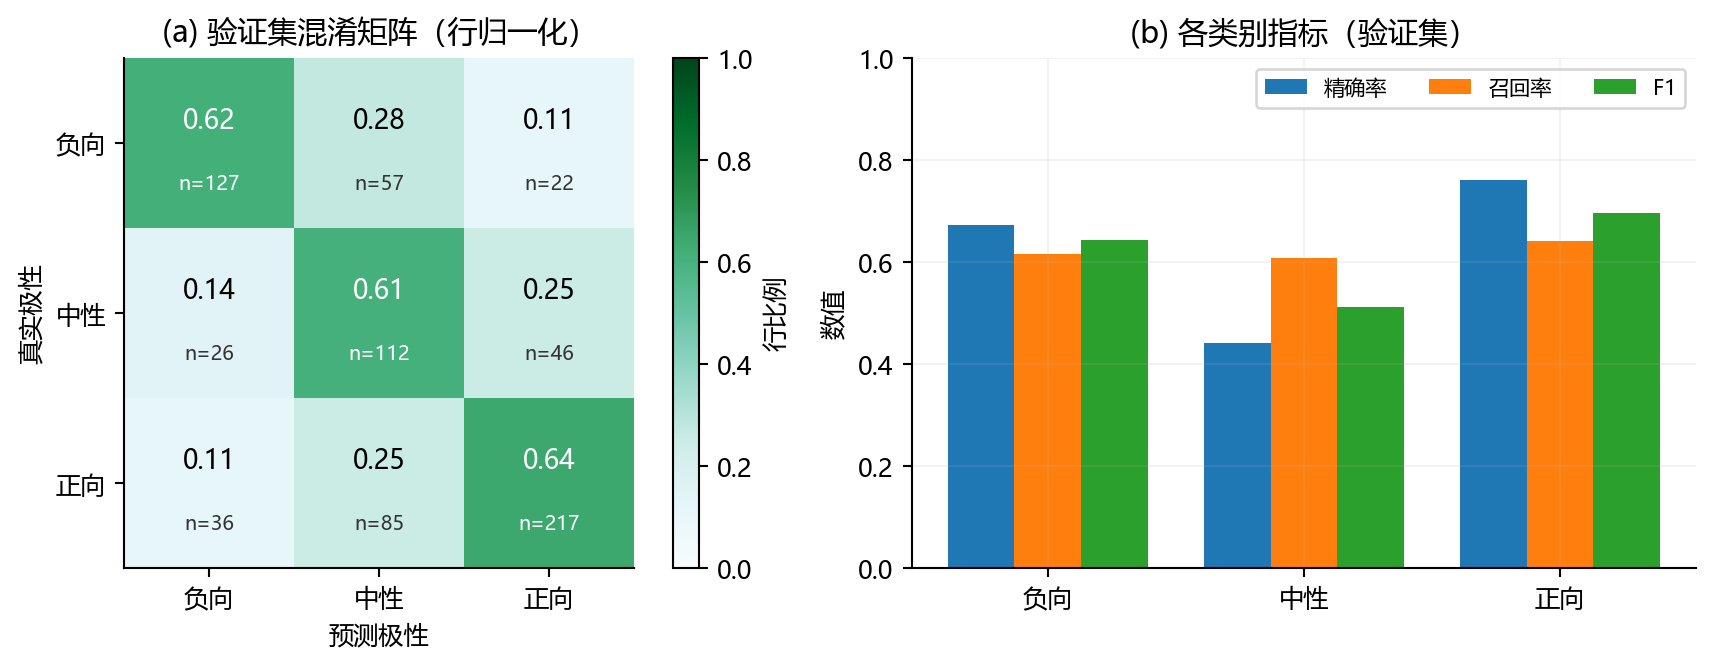
\includegraphics[width=.92\linewidth]{figures/q3_performance.png}
\caption{验证集混淆矩阵与分类指标。}\label{q3:fig:perf}\end{figure}

\begin{table}[htbp]\centering\small
\caption{候选方案与实现对照的验证结果}\label{q3:tab:ablation}
\begin{tabular}{lrrrrr}\toprule
方案 & $J$ & Macro-F1 & MAE & AOPC差 & 种子一致率\\\midrule
仅完整输入（单种子） & 0.5470 & 0.6073 & 0.6030 & --- & --- \\
无内容区打包对照 & 0.5468 & 0.6073 & 0.6048 & --- & --- \\
C0：子集训练 & 0.557 & 0.6170 & 0.5954 & 0.107 & 84.0\% \\
V1：采样与遮挡 & 0.553 & 0.6112 & 0.5869 & 0.130 & 77.8\% \\
V2：增加容量 & 0.553 & 0.6128 & 0.6010 & 0.112 & 79.2\% \\
V3：单调正则 & 0.559 & 0.6192 & 0.6011 & 0.124 & 75.7\% \\
\bottomrule\end{tabular}\end{table}
V1未通过预测指标与缺失状态性能门槛，V2未通过预测指标门槛，V3未通过缺失状态性能门槛；三者的解释AOPC差均达到门槛。据此选择C0作为最终SAP预测器，后续贡献分解和附件4推理均使用该模型。内容区打包与全序列编码的各单种子$J$平均值分别为0.542和0.539。表中仅完整输入对照采用单种子，其余方案采用三种子集成；种子一致率指主要参考模态的两两一致率平均值。
整模态删除给出模态重要性的独立证据：C0去文本后的Macro-F1为0.4150，而去语音、去视觉后分别为0.6092与0.5974，相对完整输入的0.6170，文本删除造成的下降最大，与联盟分解中文本主导的结论一致。仅用完整输入训练的单种子模型去文本后降至0.2904；两者集成规模不同，该差值同时包含训练方案与集成的影响。全缺失条件仅用于输入状态诊断，其预测仍可利用保留的内容长度。

\paragraph{模态作用差异}
空集价值为-0.687，全模态价值为0.542，单模态联盟中文本为0.382、语音为-0.651、视觉为-0.637；三模态平均Shapley贡献为文本+1.105、语音+0.068、视觉+0.056，96条子集中分类主参考模态为文本86条、语音3条、视觉7条。
图\ref{q3:fig:coal}显示，文本的平均Shapley贡献为$+1.105$，构成预测的主导信息来源；语音与视觉分别贡献$+0.068$与$+0.056$，在三模态协同中提供补充信息，主参考模态分布与贡献排序一致。样本层的正负贡献与主参考模态另行保留，以刻画个体差异。效率性残差不超过$8.9\times10^{-16}$，满足Shapley效率性公理。
\begin{figure}[htbp]\centering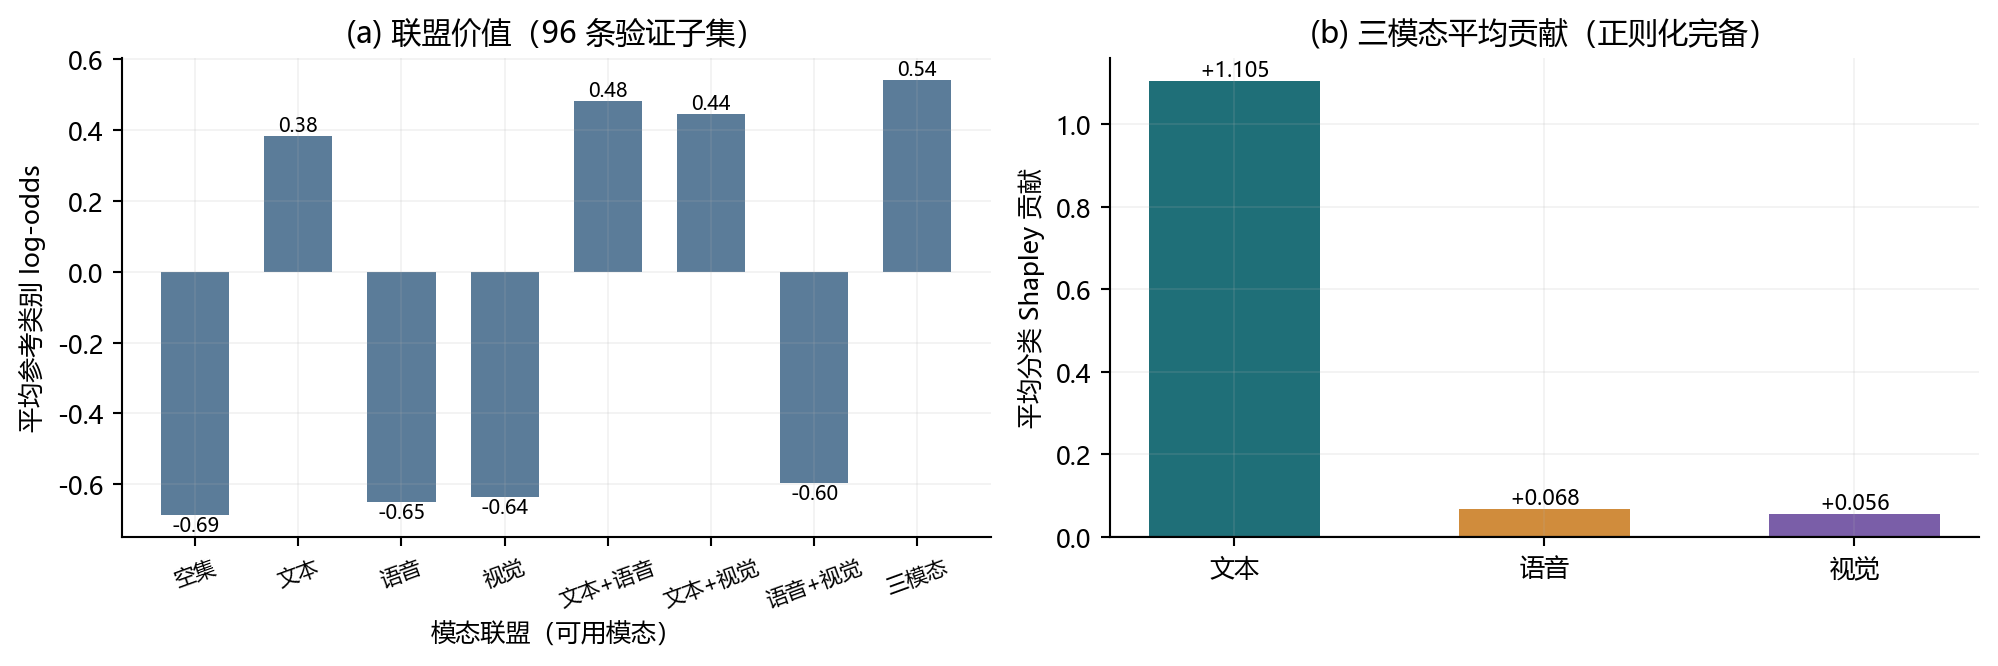
\includegraphics[width=.94\linewidth]{figures/q3_coalition_value.png}
\caption{模态联盟的平均分类价值与三模态平均Shapley贡献。}\label{q3:fig:coal}\end{figure}

\paragraph{局部证据与解释检验}
位置级证据由输入干预直接度量：96条验证样本共完成3397个局部块干预，文本、语音与视觉的平均绝对log-odds响应分别为0.377、0.015与0.025，与模态级贡献的结论一致，均以文本为主。典型样本的逐块分布见图\ref{q3:fig:card1}，累计删除结果见图\ref{q3:fig:faith}。
按块数10\%、20\%、30\%三个目标档位累计删除时，高分块引起的参考类别概率下降分别为0.187、0.226、0.241，随机块为0.075、0.111、0.148，低分块为-0.014、0.006、0.038；高分块与随机块的样本级配对差为0.1068（95\%区间[0.0887,0.1259]），实际覆盖率为14.41\%、24.03\%、35.49\%。条件充分性在最高档的绝对概率偏差为0.1608，表明主要模态中被舍弃的片段对预测仍有贡献。图\ref{q3:fig:faith}(b)给出解释方法的对照结果：B1/B2/B3三种基线下的主模态一致率分别为100.00\%、90.62\%与87.50\%，绝对贡献排序的Spearman相关为0.812与0.625，主要参考模态的判定不依赖具体基线。同一删除协议在强度回归头上给出相同的排序：删除高分块10\%、20\%、30\%时强度的绝对变化为0.399、0.468与0.499，删除低分块为0.142、0.192与0.227，两组差距随删除比例扩大，局部证据排序对连续强度输出同样成立。在主参考模态为文本的86条样本中，最高分证据块完全由功能词或标点构成的比例为17.4\%，低于全部文本块基线的30.5\%，配对差为-0.130（95\%区间[-0.212,-0.046]），最高分证据落点集中在实词上。
\begin{figure}[htbp]\centering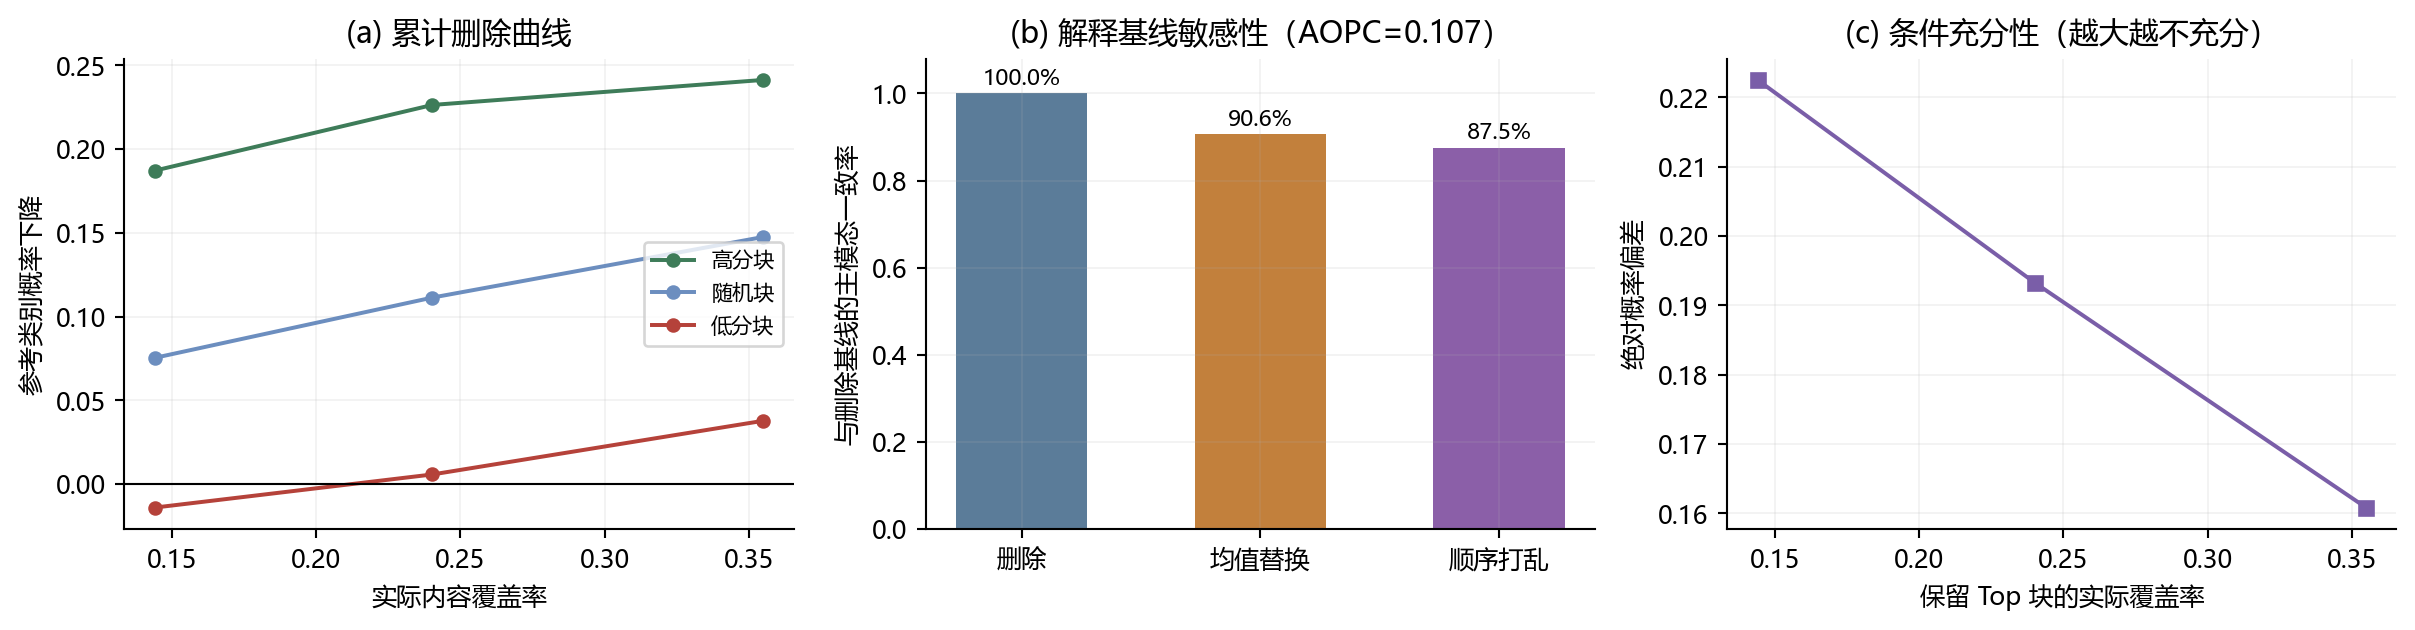
\includegraphics[width=\linewidth]{figures/q3_faithfulness.png}
\caption{高分、随机与低分块累计删除对比、基线敏感性及条件充分性。}\label{q3:fig:faith}\end{figure}
训练随机性与解释基线分别检验解释的稳定性：三种子两两的主参考模态一致率为82.29\%、83.33\%与86.46\%，B1/B2/B3三种基线下的主模态一致率分别为100.00\%、90.62\%与87.50\%。输入删除能够稳定识别对当前预测作用较强的片段；上述96条样本同时参与候选比较，置信区间描述该验证子集上的配对差异。

\paragraph{错误分布与归因分析}
验证集共272条误判，其中214条涉及中性，占78.7\%。按真实分组看：中性组错误率39.1\%（184条），非中性且|强度|<0.5的弱情感组错误率60.5\%（147条），|强度|≥0.5的强情感组错误率28.0\%（397条）。错误随情感强度降低而集中，说明零点附近的类别判别比强情感的方向判断更困难。

在96条解释样本中，低强度组与高强度组的解释不稳定率分别为31.7\%和23.6\%，覆盖正确与错误预测两类样本，给出解释稳定性在不同强度水平上的分布。错误分析将改进重点指向中性边界与弱情感区间的表征增强。

\paragraph{附件4全量结果}
附件4全部20条样本的预测分布为中性7条、负向7条、正向6条，分类主参考模态为文本19条、视觉1条。图\ref{q3:fig:a4}给出全量预测、模态份额和种子间波动，表\ref{q3:tab:all20}列出逐条数值。20条样本的强度三种子标准差均值为0.105，最大为0.410（附件4\_10）。第13条的视觉分支不可用，其视觉份额标记为NA，其余两个模态照常给出贡献；4-04与4-19的预测极性与强度方向不一致，属于独立双头结构下的输出分歧，两个任务分别保留各自的预测与贡献分解。
\begin{figure}[htbp]\centering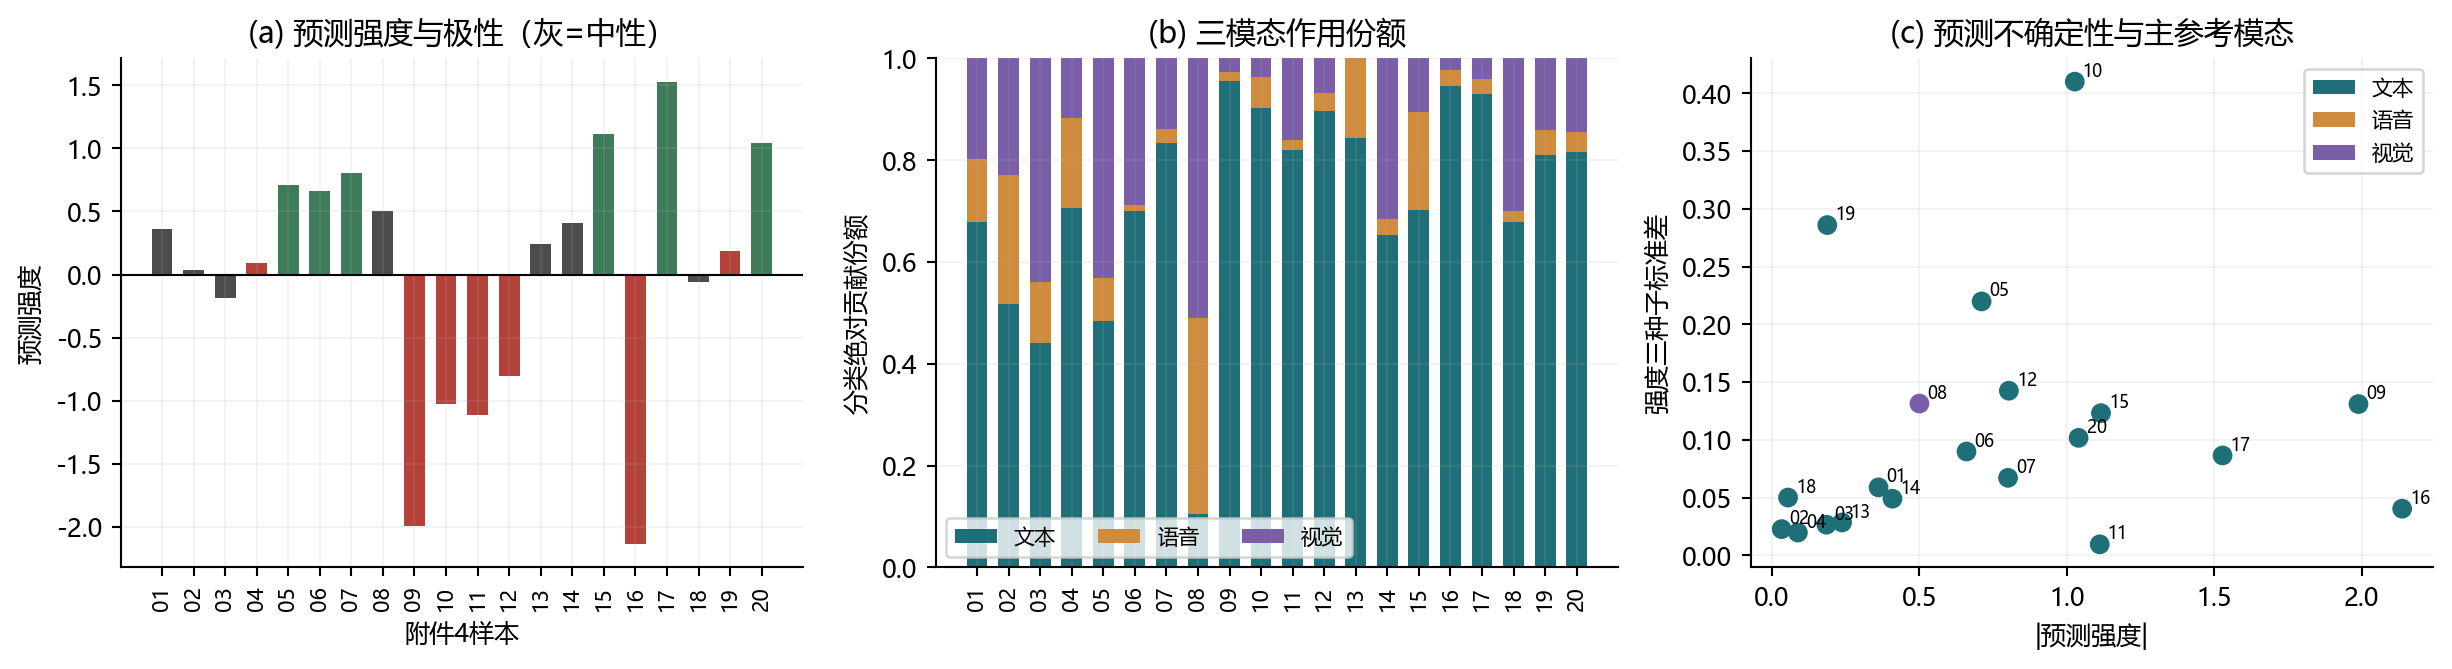
\includegraphics[width=\linewidth]{figures/q3_a4_overview.png}
\caption{附件4全部20条样本的情感预测、模态作用份额与种子间波动。}\label{q3:fig:a4}\end{figure}
\begin{table}[htbp]\centering\small
\caption{附件4全量预测与分类模态作用份额}\label{q3:tab:all20}
\begin{tabular}{clrrrrl}\toprule
编号 & 极性 & 强度 & 文本份额 & 语音份额 & 视觉份额 & 主模态\\\midrule
4-01 & 中性 & +0.362 & 0.678 & 0.124 & 0.198 & 文本 \\
4-02 & 中性 & +0.034 & 0.518 & 0.254 & 0.229 & 文本 \\
4-03 & 中性 & -0.185 & 0.441 & 0.119 & 0.440 & 文本 \\
4-04 & 负向 & +0.089 & 0.705 & 0.178 & 0.116 & 文本 \\
4-05 & 正向 & +0.711 & 0.484 & 0.085 & 0.432 & 文本 \\
4-06 & 正向 & +0.660 & 0.699 & 0.014 & 0.287 & 文本 \\
4-07 & 正向 & +0.801 & 0.833 & 0.029 & 0.138 & 文本 \\
4-08 & 中性 & +0.501 & 0.106 & 0.384 & 0.510 & 视觉 \\
4-09 & 负向 & -1.989 & 0.955 & 0.018 & 0.027 & 文本 \\
4-10 & 负向 & -1.027 & 0.903 & 0.060 & 0.037 & 文本 \\
4-11 & 负向 & -1.112 & 0.820 & 0.020 & 0.160 & 文本 \\
4-12 & 负向 & -0.804 & 0.897 & 0.036 & 0.067 & 文本 \\
4-13 & 中性 & +0.238 & 0.844 & 0.156 & NA & 文本 \\
4-14 & 中性 & +0.409 & 0.654 & 0.031 & 0.315 & 文本 \\
4-15 & 正向 & +1.116 & 0.703 & 0.192 & 0.105 & 文本 \\
4-16 & 负向 & -2.137 & 0.946 & 0.031 & 0.022 & 文本 \\
4-17 & 正向 & +1.528 & 0.930 & 0.029 & 0.040 & 文本 \\
4-18 & 中性 & -0.055 & 0.679 & 0.021 & 0.300 & 文本 \\
4-19 & 负向 & +0.188 & 0.809 & 0.049 & 0.141 & 文本 \\
4-20 & 正向 & +1.040 & 0.816 & 0.040 & 0.144 & 文本 \\
\bottomrule\end{tabular}\end{table}
\file{pred\_附件4.csv}保存预测及分类、强度的有符号贡献；\file{explain\_附件4.csv}按样本和模态保存证据片段、时间与媒体索引，共60行，包含不可用状态；\file{local\_blocks\_附件4.csv}保存全部逐块响应。

\paragraph{典型样本与证据回映}
选取附件4第1条展示完整解释链条。第1条预测为中性，强度+0.362，主要参考模态为文本（份额0.678），最高分证据片段为\textit{the timing}，估计时间2.62--3.00\,s。 图\ref{q3:fig:card1}同时展示预测结果、三模态作用程度、主要模态的逐块响应与原始关键帧；响应的正负分别对应支持和抑制作用。
\begin{figure}[htbp]\centering\includegraphics[width=.90\linewidth]{figures/q3_card_01.png}
\caption{附件4第1条解释卡：预测、模态份额、局部片段重要性与关键证据定位。}\label{q3:fig:card1}\end{figure}
回映覆盖情况如下：20条样本的重新分词序列均与官方词元一致，482个原词中478个获得CTC时间区间；59条可用模态证据中58条完成时间回映，时间区间由CTC词级对齐给出，未获得词区间的证据以锚点索引记录。第13条的视觉特征不可用，其解释保留文本与语音贡献，并在全量文件中标记为视觉NA。

本模型把情感预测分解为可复核的模态贡献与局部响应，并通过词级时间区间连接到原始素材：Shapley值度量指定模型与基线下的作用差异，删除实验检验局部证据与预测响应的一致性。两项分析在同一预测器上完成，因此解释结论可直接对应该模型的决策过程。
\FloatBarrier
